\documentclass[tese_patricia]{subfiles}% !TeX spellcheck = pt_BR

\begin{document}
%\nomenclature[B,01]{$\velocity$}{Vetor de velocidade com componentes $u_1$, $u_2$ e $u_3$;}
%\nomenclature[B,02]{$\time$}{Instante de tempo arbitrário;}
%\nomenclature[B,03]{$\density$}{Massa específica do fluido;}
%\nomenclature[B,04]{$dV$}{Volume de controle infinitesimal;}
%\nomenclature[B,05]{$dA_i$}{Área referente à face ortogonal ao eixo $y_i$ do volume de controle infinitesimal;}
%\nomenclatura[B,06]{$dy_i$}{Dimensão do volume de controle infinitesimal na direção $y_i$;}
%\nomenclatura[B,07]{$\mathbf{F}$}{Vetor da resultante das forças externas atuando em um volume de controle infinitesimal, com componentes $F_1$, $F_2$ e $F_3$}
%\nomenclatura[B,08]{$\stressTensor$}{Tensor de tensões de Cauchy de componentes $\sigma_ij$ com $i,j = 1,2,3$;}
%\nomenclatura[B,09]{$\mathbf{b}$}{Vetor forças de campo por unidade de volume com componentes $b_1$, $b_2$ e $b_3$;}
%\nomenclatura[B,10]{$\mathbf{q}$}{Vetor resultante das forças externas por unidade de volume com componentes $q_1$, $q_2$ e $q_3$;}
%\nomenclatura[B,11]{$\sbodyforce$}{Vetor que representa a força de campo por unidade de massa, com componentes $f_1$, $f_2$ e $f_3$;}
%\nomenclature[B,12]{$\press$}{Campo de pressões de um escoamento;}
%\nomenclature[B,13]{$\viscosity$}{Viscosidade dinâmica do fluido;}
%\nomenclature[B,14]{$\straintensor(\bullet)$}{Tensor taxa de deformação infinitesimal;}
%\nomenclature[B,15]{$\domain$}{Domínio espacial ou domínio atual do escoamento do fluido;}
%\nomenclature[B,16]{$\nsd$}{Dimensão espacial;}
%\nomenclature[B,17]{$\boundary$}{Contorno do domínio espacial que define o escoamento do fluido;}
%\nomenclature[B,18]{$\boundaryD$}{Porção do contorno com condições de contorno de Dirichlet;}
%\nomenclature[B,19]{$\boundaryN$}{Porção do contorno com condições de contorno de Neumann;}
%\nomenclature[B,20]{$\totalTime$}{Intervalo de tempo total da análise;}
%\nomenclature[B,21]{$\velocityD$}{Vetor de velocidades prescritas;}
%\nomenclature[B,22]{$\surfaceLoad$}{Forças de superfície prescritas;}
%\nomenclature[B,23]{$\snormal$}{Vetor normal ao contorno do domínio computacional;}
%\nomenclature[B,24]{$\domainMat$}{Domínio inicial ou material do escoamento do fluido;}
%\nomenclature[B,25]{$\posMat$}{Vetor das coordenadas dos pontos materiais de um ponto arbitrário;}
%\nomenclature[B,26]{$\pos$}{Vetor das coordenadas atuais de um ponto arbitrário;}
%\nomenclature[B,27]{$\domainRef$}{Domínio de referência do escoamento do fluido;}
%\nomenclature[B,28]{$\posAle$}{Vetor das coordenadas de referência de um ponto arbitrário;}
%\nomenclature[B,29]{$\fmapAI(\posMat,t)$}{Função mudança de configuração do domínio material para o domínio espacial;}
%\nomenclature[B,30]{$\fmapAR(\posALE,t)$}{Função mudança de configuração do domínio de referência para o domínio espacial;}
%\nomenclature[B,31]{$\fmapRI(\posMat,t)$}{Função mudança de configuração do domínio material para o domínio de referência;}	
%\nomenclature[B,32]{$\velocityALE$}{Velocidade dos pontos de referência;}
%\nomenclature[B,33]{$\FmapAI$}{Matriz jacobiana da função de mapeamento $\fmapAI(\posMat,t)$;}
%\nomenclature[B,34]{$\FmapAR$}{Matriz jacobiana da função de mapeamento $\fmapAR(\posALE,t)$;}
%\nomenclature[B,35]{$\FmapRI$}{Matriz jacobiana da função de mapeamento $\fmapRI(\posMat,t)$;}
%\nomenclature[B,36]{$g,g^{*},g^{**}$}{Grandeza física escalar na configuração espacial, de referência e material respectivamente;}
%\nomenclature[B,37]{$\usolution$}{Espaço vetorial das funções aproximadoras do campo de velocidades;}
%\nomenclature[B,38]{$\psolution$}{Espaço vetorial das funções aproximadoras do campo de pressões;}
%\nomenclature[B,39]{$\uweighting$}{Espaço vetorial das funções ponderadoras do campo de velocidades;}
%\nomenclature[B,40]{$\pweighting$}{Espaço vetorial das funções ponderadoras do campo de pressões;}
%\nomenclature[B,41]{$\utest$}{Função ponderadora pertencente ao espaço $\uweighting$;}
%\nomenclature[B,42]{$\ptest$}{Função ponderadora pertencente ao espaço $\pweighting$;}
%\nomenclature[B,43]{$(\bullet)^h$}{O superscrito $h$ indica, em todos os casos, a discretização em elementos finitos da variável;}
%\nomenclature[B,44]{$\domainE$}{Domínio computacional de um elemento finito;}
%\nomenclature[B,45]{$\nel$}{Número de subdomínios do domínio discreto;}
%\nomenclature[B,46]{$\nnos$}{Número de nós ou pontos de controle do domínio discreto;}
%\nomenclature[B,47]{$\boundary^{b}$}{Domínio computacional de um elemento finito no contorno;}
%\nomenclature[B,48]{$\neb$}{Número de subdomínios do domínio discreto no contorno;}
%\nomenclature[B,49]{$\shapef$}{Função de forma da discretização do domínio;}
%\nomenclature[B,50]{$(\bullet)_A$}{O subscrito $A$ indica, em todos os casos, que se trata da variável respectiva ao nó $A$ da malha de elementos finitos;}
%\nomenclature[B,51]{$\SUPG$}{Parâmetro de estabilização do método \textit{Streamline-Upwind/Petrov-Galerkin} (SUPG);}
%\nomenclature[B,52]{$\PSPG$}{Parâmetro de estabilização do método \textit{Pressure-Stabilizing/Petrov-Galerkin} (PSPG);}
%\nomenclature[B,53]{$\LSIC$}{Parâmetro de estabilização do método \textit{Least-Squares on the Incompressibility Constraint} (LSIC);}
%\nomenclature[B,54]{$\resMom$}{Resíduo da equação da quantidade de movimento;}
%\nomenclature[B,55]{$\resPre$}{Resíduo da equação da continuidade;}
%\nomenclature[B,56]{$\NNSM$}{Resíduo do vetor semidiscreto da equação da quantidade de movimento;}
%\nomenclature[B,57]{$\NNSC$}{Resíduo do vetor semidiscreto da equação da continuidade;}
%\nomenclature[B,58]{$\Acceleration$}{Vetor nodal dos graus de liberdade respectivo a aceleração;}
%\nomenclature[B,59]{$\Velocity$}{Vetor nodal dos graus de liberdade respectivo a velocidade;}
%\nomenclature[B,60]{$\Press$}{Vetor nodal dos graus de liberdade respectivo a pressão;}
%\nomenclature[B,61]{$\matrixQ$}{Matriz Jacobiana do elemento;}
%\nomenclature[B,62]{$\coordAdimen$}{Vetor das coordenadas paramétricas adimensionais do elemento com componentes $\xi$, $\eta$ $\zeta$;}
%\nomenclature[B,63]{$\matrixD$}{Matriz que realiza mudança de escala em $\matrixQ$ para levar em conta o grau polinomial das funções de forma;}
%\nomenclature[B,64]{$\matrixQhat$}{Matriz jacobiana escalonada;}
%\nomenclature[B,65]{$\RGN$}{Comprimento direcional do elemento finito;}
%\nomenclature[B,66]{$\rRGN$}{Vetor unitário no sentido do gradiente da intensidade da velocidade;}
%\nomenclature[B,67]{$\matrixG$}{Tensor métrico do elemento;}
%\nomenclature[B,68]{$h_{min}$}{Mínimo comprimento de escala do elemento finito;}
%\nomenclature[B,69]{$h_{max}$}{Máximo comprimento de escala do elemento finito;}
%\nomenclature[B,70]{$\lambda_{min},\lambda_{max}$}{mínimo e máximo autovalor da matriz $\matrixG$;}
%\nomenclature[B,71]{$\SUGNi,\SUGNii,\SUGNiii$}{Parâmetros da estabilização SUPG/PSPG/LSIC correspondentes aos termos convectivos, inerciais e viscosos, respectivamente;}
%\nomenclature[B,72]{$\rRGN_{reg}$}{Vetor unitário no sentido do gradiente da intensidade da velocidade do fluido modificado de maneira a evitar problemas numéricos devido divisão por zero;}
%\nomenclature[B,73]{$\varepsilon$}{Constante pequena utilizada no cálculo de $\rRGN_{reg}$;}
%\nomenclature[B,74]{$t_{n}$}{é o tempo atual, ou seja, o instante n-ésimo no qual a solução foi calculada.;}
%\nomenclature[B,75]{$t_{n+1}$}{é o próximo instante de tempo, ou seja, o instante $n+1$ no qual solução será calculada;}
%\nomenclature[B,76]{$\alpham, \alphaf, \gamma$}{Parâmetros reais do esquema de integração temporal $\alpha$-generalizado;}
%\nomenclature[B,77]{$\specRadius$}{Raio espectral da matriz de amplificação;}
%\nomenclature[B,78]{$\Reynolds$}{Número de Reynolds;}
%\nomenclature[B,79]{$\velocinfty$}{Velocidade de referência;}
%\nomenclature[B,80]{$L$}{Comprimento característico/de referência do escoamento;}
%\nomenclature[B,81]{$\kviscosity$}{Viscosidade cinemática do fluido;}
%\nomenclature[B,82]{$F_L, F_D$}{Forças de sustentação e arrasto, respectivamente;}
%\nomenclature[B,83]{$C_L, C_D$}{Coeficiente de sustentação e arrasto, respectivamente;}
%\nomenclature[B,84]{$\Strouhal$}{Número de Strouhal;}
%\nomenclature[B,85]{$f_v$}{Frequência de desprendimento dos vórtices;}

% ---------------------------------------------------------- 
% Métodos de \part{\part{malhas}} sobrepostas
% ----------------------------------------------------------
\chapter[Dinâmica dos fluidos computacional]{Dinâmica dos fluidos computacional}
\label{capitulo:Cap2}
% ----------------------------------------------------------

O escoamento isotérmico de um fluido newtoniano é descrito pelas equações advindas da conservação da quantidade de movimento, ou de Navier-Stokes, e da conservação de massa. Nos casos em que ocorram variações significativas de temperatura ou em escoamentos compressíveis, a equação da conservação da energia deve ser incorporada ao sistema. Essas equações, em conjunto com a relação constitutiva, formam um sistema de equações diferenciais não lineares que descrevem o comportamento do escoamento no tempo e no espaço. 

Neste trabalho, são investigados escoamentos incompressíveis, isotérmicos e com contornos móveis. As seções seguintes apresentam a abordagem adotada para a resolução desse tipo de problema, bem como sua implementação computacional. Adota-se uma descrição Euleriana-Lagrangiana Arbitrária (ALE) para representar as equações, e a discretização espacial é realizada por meio do método dos elementos finitos (FEM) ou da análise isogeométrica (IGA).

Para tratar questões numéricas recorrentes nesse tipo de equações, como as oscilações espúrias em casos de convecção dominante, típicas da aplicação direta do método dos resíduos ponderados na formulação clássica de Galerkin, emprega-se a metodologia Streamline Upwind/Petrov-Galerkin (SUPG). Além disso, a estabilização Pressure-Stabilizing/Petrov-Galerkin (PSPG) é aplicada com o objetivo de contornar as condições de \textit{Ladyzhenskaya–Babuška–Brezzi} (LBB) associadas aos escoamentos incompressíveis, permitindo o uso estável de um mesmo espaço de funções de aproximação para pressão e velocidade. A integração temporal é realizada por meio do método $\alpha$-generalizado.

Ao final deste capítulo, apresenta-se um algoritmo que descreve o esquema de solução computacional adotado neste trabalhos para a mecânica dos fluidos, seguido da simulação de casos clássicos para a verificação da metodologia proposta.

\section{Equações governantes na descrição Euleriana} 


\subsection{Equação da conservação da massa}

Para obter a equação da conservação da massa na descrição espacial, considera-se um volume de controle infinitesimal fixo no espaço, permeável à matéria e submetido a um escoamento com velocidade $\velocity$, cujos componentes são $u_1$, $u_2$ e $u_3$ (conforme a Fig. \ref{fig:volInf_fluxoMassa}). Para um intervalo de tempo infinitesimal $\deriv t$, a lei da conservação da massa estabelece que a variação de massa dentro do volume de controle deve ser igual ao balanço do fluxo líquido de massa que atravessa suas fronteiras, podendo ser expressa matematicamente da seguinte forma:

\begin{figure}[htb!]
	\centering 
	%\vspace{-1em} % Diminui o espaço antes da figura
	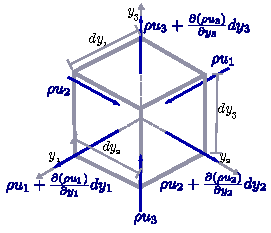
\includegraphics[scale=1.5,trim=0cm 0.0cm 0cm 0.0cm, clip=true]{Imagens/Cap2/volInf_fluxoMassa.pdf}	
	\caption{Volume de controle infinitesimal: Fluxo de massa}
	\label{fig:volInf_fluxoMassa}
	%\vspace{-1em} % Diminui o espaço antes da figura
\end{figure}


\begin{align}
	\begin{split}
	\frac{\partial \density}{\partial t}\deriv V =& \left(\density u_1 \deriv A_{1}  +  \density u_2 \deriv A_{2} + \density u_3  \deriv A_{3} \right) - \\  &\left(\left(\density u_1 + \frac{\partial \density u_1}{\partial y_1}\deriv y_1 \right)\deriv A_{1} + \left(\density u_2+ \frac{\partial \density u_2}{\partial y_2}\deriv y_2 \right) \deriv A_{2} + \left(\density u_3 + \frac{\partial \density u_3}{\partial y_3}\deriv y_3 \right) \deriv A_{3}\right), \label{eq:conser_massa_0} 
	\end{split}
\end{align}

\noindent com $\density$ sendo a densidade de massa do fluido e $\deriv A_{i}$ a área referente à face ortogonal ao eixo $y_i$. Considerando que $\deriv V = \deriv y_1 \deriv y_2 \deriv y_3 = \deriv y_1 \deriv A_1 = \deriv y_2 \deriv A_2 = \deriv y_3 \deriv A_3 $  e manipulando-se algebricamente a Eq. \ref{eq:conser_massa_0}, resulta:

\begin{align}
	\frac{\partial \density}{\partial t} = - \frac{\partial \density u_{1}}{\partial y_1} - \frac{\partial \density u_{2}}{\partial y_2}- \frac{\partial \density u_{3}}{\partial y_3}.
\end{align}

Para escoamentos incompressíveis, quando $\density$ é constante, a equação fica reduzida a:

\begin{align}
	 \frac{\partial u_{1}}{\partial y_1} + \frac{\partial u_{2}}{\partial y_2} + \frac{\partial u_{3}}{\partial y_3} = 0, 
\end{align} 

\noindent ou ainda:

\begin{align}
	\divergence \cdot \velocity = 0.
	\label{eq:conser_massa_incom} 
\end{align} 
\noindent onde $\divergence \cdot (\velocity)$ é o divergente de $\velocity$ em relação às coordenadas Eulerianas $\ePosition$.

\subsection{Equação da quantidade de movimento}


Para um volume de controle infinitesimal, a lei da conservação da quantidade de movimento afirma que a variação temporal da quantidade de movimento no interior do volume é determinada pela diferença entre o fluxo de quantidade de movimento que entra e o que sai pelas suas fronteiras, somada à resultante das forças aplicadas sobre o volume de controle.

Para chegar-se à equação da quantidade de movimento em sua forma conservativa e seguindo a descrição espacial, inicia-se com a avaliação das forças que atuam sobre um volume de controle infinitesimal no instante atual, como ilustrado na Fig. \ref{fig:volInf_tensao}, onde são mostradas apenas as componentes que atuam na direção $y_1$. Somando-se vetorialmente as componentes de forças externas e internas na direção $y_1$, chega-se na seguinte relação:

\begin{align}
	\begin{split}
	F_1 =& -\left(\stress_{11}\deriv y_2 \deriv y_3 + \stress_{12}\deriv y_1 \deriv y_3 + \stress_{13}\deriv y_1 \deriv y_2\right) + \\ & \left(\left(\stress_{11} + \frac{\partial \stress_{11}}{\partial y_1}\deriv y_1 \right)\deriv y_2 \deriv y_3 + \left(\stress_{12}+ \frac{\partial \stress_{12}}{\partial y_2}\deriv y_2\right)\deriv y_1 \deriv y_3 + \left(\stress_{13}+ \frac{\partial \stress_{13}}{\partial y_3}\deriv y_3\right)\deriv y_1 \deriv y_2\right) + \\& b_{1}\deriv y_1 \deriv y_2 \deriv y_3, \label{eq:equil_forca_y1} 
	\end{split}
\end{align}	

\noindent onde $F_1$ representa a resultante das forças externas na direção $y_1$; $\stress_{ij}$ são as componentes $ij$ do tensor das tensões de Cauchy ($\stressTensor$); e $b_1$ representa a componente do vetor força de campo por unidade de volume na direção $y_1$. Dividindo-se Eq. \ref{eq:equil_forca_y1} por $\deriv V$ e efetuando as subtrações, tem-se a componente de força resultante por unidade de volume na direção de $y_1$ ($q_1$):

\begin{align}
		q_1 =\frac{\partial \stress_{11}}{\partial y_1} + \frac{\partial \stress_{12}}{\partial y_2} + \frac{\partial \stress_{13}}{\partial y_3} + b_{1}.
\end{align}	

\begin{figure}[htb!]
	\centering 
	%\vspace{-1em} % Diminui o espaço antes da figura
	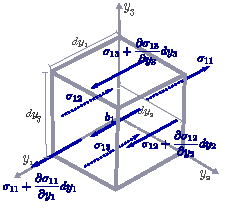
\includegraphics[scale=1.5,trim=0cm 0.0cm 0cm 0.0cm, clip=true]{Imagens/Cap2/volInf_tensao.pdf}	
	\caption{Volume de controle infinitesimal: Componentes de força na direção $y_1$}
	\label{fig:volInf_tensao}
	%\vspace{-1em} % Diminui o espaço antes da figura
\end{figure}

Seguindo a mesma ideia para as direções $y_2$ e $y_3$, escreve-se:

\begin{align}
	q_2 =\frac{\partial \stress_{21}}{\partial y_1} + \frac{\partial \stress_{22}}{\partial y_2} + \frac{\partial \stress_{23}}{\partial y_3} + b_{2},
\end{align}	
e
\begin{align}
	q_3 =\frac{\partial \stress_{31}}{\partial y_1} + \frac{\partial \stress_{32}}{\partial y_2} + \frac{\partial \stress_{33}}{\partial y_3} + b_{3},
\end{align}

\noindent ou ainda, de forma simbólica:

\begin{align}
	\mathbf{q} = \divergence \cdot \stressTensor + \mathbf{b}.
\end{align}


Realizando-se o balanço da quantidade de movimento no volume de controle infinitesimal da Fig. \ref{fig:volInf_consQtdeMov}, e aplicando-se o princípio da conservação da quantidade de movimento, pode-se escrever:


\begin{align}
	\begin{split}
	\frac{\partial \density \velocity}{\partial t}\deriv V =& u_1\density \velocity \deriv A_1 + u_2\density \velocity \deriv A_2 + u_3 \density \velocity \deriv A_3 - \\
	 & \left(\left(u_1 \density \velocity + \frac{\partial u_1 \density \velocity}{\partial y_1}\deriv y_1 \right)\deriv A_1 + \left(u_2 \density \velocity + \frac{\partial u_2 \density \velocity}{\partial y_2}\deriv y_2 \right)\deriv A_2 \right. + \\ & \left.   \left(u_3 \density \velocity + \frac{\partial u_3 \density \velocity}{\partial y_3}\deriv y_3 \right)\deriv A_3\right) + \mathbf{q} \deriv V,
	\label{eq:QM_0} 
	\end{split}
\end{align}	

\noindent dividindo-se a Eq. \ref{eq:QM_0} por $\deriv V$ e efetuando-se as subtrações, chega-se a :

\begin{align}
		\frac{\partial \density \velocity}{\partial t} = 
		-\frac{\partial u_1 \density \velocity}{\partial y_1} 
		-\frac{\partial u_2 \density \velocity}{\partial y_2}  
		-\frac{\partial u_3 \density \velocity}{\partial y_3} + \mathbf{q},
		\label{eq:QM_1} 
\end{align}
\noindent ou ainda, considerando que $\density$ é constante:
\begin{align}
	\density\left(\frac{\partial\velocity}{\partial t} + \divergence \cdot \left(\velocity\otimes\velocity\right) - \sbodyforce \right) - \divergence \cdot \stressTensor  &= \vzero, \label{eq:QM_2} 
\end{align}

\noindent onde $\sbodyforce = \mathbf{b}/\density$ representa a força de campo por unidade de massa.

\begin{figure}[htb!]
	\centering 
	%\vspace{-1em} % Diminui o espaço antes da figura
	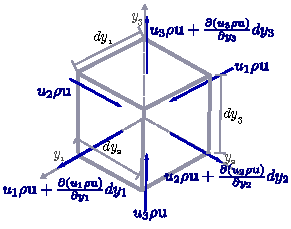
\includegraphics[scale=1.5,trim=0cm 0.0cm 0cm 0.0cm, clip=true]{Imagens/Cap2/volInf_consQtdeMov.pdf}	
	\caption{Volume de controle infinitesimal: Fluxo de quantidade de Movimento}
	\label{fig:volInf_consQtdeMov}
	%\vspace{-1em} % Diminui o espaço antes da figura
\end{figure}

Da consideração da equação da continuidade, a Eq. \ref{eq:QM_2} pode ser rescrita em sua forma convectiva como:

\begin{align}
	\density\left(\frac{\partial\velocity}{\partial t} + \left( \velocity \cdot \gradient \right)  \velocity  - \sbodyforce \right) - \divergence \cdot \stressTensor = \vzero. \label{eq:Navier-Stokes} 
\end{align}

\subsection{Relação constitutiva}
O tensor de tensões de Cauchy $\stressTensor$ é definido para fluidos newtonianos incompressíveis pela seguinte relação constitutiva:

\begin{align}
\stressTensor &= -\press \unittensor + 2\viscosity\straintensor(\velocity),\label{eq:tensor_tensoes_fluido}
\end{align}

\noindent onde $\press$ representa a pressão, $\viscosity$ a viscosidade dinâmica do fluido e $\straintensor(\bullet)$ é o tensor taxa de deformação Euleriana, definido como:


\begin{align}
\straintensor(\bullet) = \frac{1}{2}\left(\gradient (\bullet) + \gradient (\bullet)^{T}\right). 
\label{eq:tensor_taxa_defor}
\end{align}


\subsection{\sout{Modelo matemático para escoamentos incompressíveis na forma forte}}

\textcolor{red}{Sugiro colocar isso após a descrição ALE apenas....}

\sout{Seja $\domain \in \nrealspace$, com $\nsd = 1,2,3$ definindo a dimensão do domínio espacial do escoamento com contorno $\boundary = \boundaryD \cup \boundaryN$, no instante $t \in (0,\totalTime)$ (ver Fig. \ref{fig:dominioFluido}).

Para escoamentos incompressíveis isotérmicos o fluido possui movimento descrito pela equação da quantidade de movimento, ou equações de Navier-Stokes (Eq. \ref{eq:Navier-Stokes}) e da conservação de massa (Eq. \ref{eq:conser_massa_incom}). Para completar a formulação da mecânica dos fluidos, condições de contorno devem ser especificadas. Em geral, em uma dada parte do contorno espacial, condições de contorno essenciais (Dirichlet) ou naturais (Neumann) são aplicadas. Dessa forma, o escoamento é governado pelo seguinte conjunto de equações:}

\begin{equation}
	\left\{
	\begin{array}{l}
		\density\left(\frac{\partial\velocity}{\partial t} + \velocity\cdot\gradient\velocity - \sbodyforce \right) - \divergence \cdot \stressTensor = \vzero \ \textrm{em} \ \domain\\
		\divergence \cdot \velocity = 0 \ \textrm{em} \ \domain\\
		\velocity = \velocityD \ \textrm{em} \ \boundaryD \\
		\stressTensor \cdot \snormal = \surfaceLoad \ \textrm{em} \ \boundaryN,
	\end{array} \label{eq:conj_eq_DFC}
	\right.
\end{equation}

\sout{\noindent sendo $\boundaryD$ a porção do contorno com condições de contorno de Dirichlet, representadas pelo campo de velocidades $\velocityD$, e $\boundaryN$ aquela com condições de contorno de Neumann, descritas pelas forças de superfície $\surfaceLoad$. A variável $\snormal$ representa o vetor unitário normal ao contorno $\boundaryN$.}

\begin{figure}[htb!]
	\centering 
	%\vspace{-1em} % Diminui o espaço antes da figura
	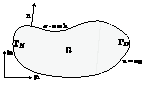
\includegraphics[scale=3.0,trim=0cm 0.0cm 0cm 0.0cm, clip=true]{Imagens/Cap2/dominioFluido.pdf}	
	\caption{\sout{Domínio para o problema da dinâmica dos fluidos computacional}}
	\label{fig:dominioFluido}
	%\vspace{-1em} % Diminui o espaço antes da figura
\end{figure}

\section{Descrição Euleriana-Lagrangiana arbitrária (ALE)} \label{capitulo:Cap2:ALE}

A descrição Lagrangiana-Euleriana arbitrária \cite{HughesLZ:1981, DoneaGH:1982} representa uma generalização das descrições puramente Lagrangiana e puramente Euleriana do movimento do contínuo. A descrição Lagrangiana fixa a atenção em pontos materiais do contínuo, enquanto que, na descrição Euleriana, considera-se uma porção fixa do espaço ocupada pelo contínuo e analisam-se os pontos materiais que passam por essa porção ao longo do tempo. Como consequência, na descrição puramente Lagrangiana a malha computacional move-se com o contínuo, enquanto que, na Euleriana, a malha computacional mantém-se espacialmente fixa e permeável ao meio contínuo. Por sua vez, na descrição Lagrangiana-Euleriana arbitrária trabalha-se com um domínio de referência que pode mover-se de maneira independente do movimento dos pontos materiais do contínuo analisado.

Para a aplicação dessa metodologia às equações governantes da mecânica dos fluidos, consideram-se três domínios contínuos, de acordo com a Fig.~\ref{fig:dominioAle}: (i) o domínio inicial, chamado de \textbf{domínio material} ($\domainMat$), definido pelas coordenadas dos pontos materiais $\posMat$ na configuração inicial; (ii) o domínio atual, chamado de \textbf{domínio espacial} ($\domain$), definido pelas coordenadas espaciais $\pos$; e, por fim, (iii) o \textbf{domínio de referência} ($\domainRef$), associado às coordenadas dos pontos de referência $\posALE$.

Considera-se neste texto, o domínio de referência, $\domainRef$, como sendo a configuração inicial da malha, enquanto que as configurações atuais, tanto da malha como do contínuo, coincidem com a referência espacial $\domain$.

As coordenadas no domínio $\domain$ podem ser mapeadas a partir do domínio inicial ($\domainMat$) ou do domínio de referência ($\domainRef$) utilizando as seguintes funções de mapeamento:  

\begin{align}
	\pos = \fmapAI(\posMat,t) = \fmapAR(\posALE,t).
\end{align}

\begin{figure}[htb!]
	\centering
	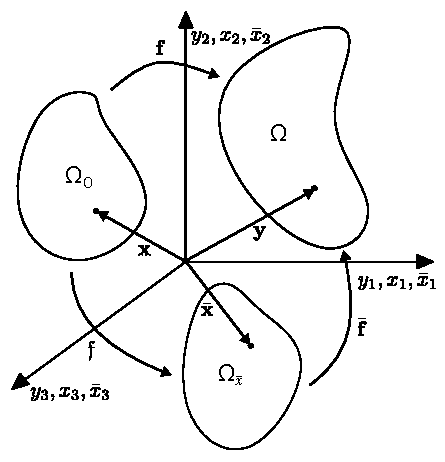
\includegraphics[scale=1.0]{Imagens/Cap2/dominioALE.pdf}	
	\caption{Descrição Lagrangiana-Euleriana arbitrária}
	\label{fig:dominioAle}
\end{figure}

Da mesma forma, o domínio de referência pode ser mapeado a partir do domínio inicial por:

\begin{align}
	\posALE = \fmapRI(\posMat,t).
\end{align}

A velocidade dos pontos da malha é calculada por:

\begin{align}
	\velocityALE = \left. \frac{\partial \fmapAR(\posALE,t)}{\partial t} \right|_{\posALE},
\end{align}

\noindent e a velocidade dos pontos materiais no instante $t$ é obtida pela derivada do vetor posição $\pos$, mantendo $\posMat$ fixo:

\begin{align}
	\velocity = \left. \frac{\partial \fmapAI(\posMat,t)}{\partial t} \right|_{\posMat} = \left. \frac{\partial \pos(\posMat,t)}{\partial t} \right|_{\posMat}.
\end{align}


As matrizes jacobianas dos mapeamentos considerando a dependência do espaço e do tempo são dadas por:

\begin{equation} 
	\FmapAI = \frac{\partial \left(\fmapAI(\posMat,t),t\right)}{\partial (\posMat,t)}=
	\begin{bmatrix}
		\frac{\partial {\pos}}{\partial {\posMat}} & \velocity \\
		\vzero^T & 1 \\
	\end{bmatrix}
	\text{,}
\end{equation}

\begin{equation} 
	\FmapAR = \frac{\partial \left(\fmapAR(\posALE,t),t\right)}{\partial (\posALE,t)}=
	\begin{bmatrix}
		\frac{\partial {\pos}}{\partial {\posALE}} & \velocityALE \\
		\vzero^T & 1 \\
	\end{bmatrix}
	\text{,}
\end{equation}

e

\begin{equation}
	\FmapRI = \frac{\partial \left({\fmapRI}(\posMat,t),t\right)}{\partial (\posMat,t)}=
	\begin{bmatrix}
		\frac{\partial {\posALE}}{\partial {\posMat}} & \mathbf{w} \\
		\vzero^T & 1 \\
	\end{bmatrix}
	\text{,}
\end{equation}

\noindent sendo $\mathbf{w} = \left. \frac{\partial \posALE}{\partial t} \right|_{\posMat}$.


Considerando que $\fmapAI\left(\posMat,t\right) = \fmapAR \circ \fmapRI$, pode-se escrever:

\begin{align}
	\frac{\partial(\fmapAI(\posMat,t),t)}{\partial(\posMat,t)} = \frac{\partial(\fmapAR(\posALE,t),t)}{\partial(\posALE,t)} \cdot \frac{\partial(\fmapRI(\posMat,t),t)}{\partial(\posMat,t)},
\end{align}

\noindent que pode ser rescrita como:

\begin{align}
	\begin{bmatrix}
		\frac{\partial {\pos}}{\partial {\posMat}} & \velocity \\
		\vzero^T & 1 \\
	\end{bmatrix}
	=
	\begin{bmatrix}
		\frac{\partial {\pos}}{\partial {\posALE}} & \velocityALE \\
		\vzero^T & 1 \\
	\end{bmatrix}
	\cdot
	\begin{bmatrix}
		\frac{\partial {\posALE}}{\partial {\posMat}} & \mathbf{w} \\
		\vzero^T & 1 \\
	\end{bmatrix} .
\end{align}

Dessa forma, pode-se estabelecer uma relação entre a velocidade da malha e a velocidade do ponto material:

\begin{align}
	\velocity = \velocityALE + \frac{\partial{\pos}}{\partial{\posALE}}\cdot \mathbf{w}. \label{eq:vel_rel_mat_ALE}
\end{align}

Supondo agora uma grandeza física escalar, denominada $g(\pos,t)$ na configuração espacial, de $g^{*}(\posALE,t)$ na configuração de referência e $g^{**}(\posMat,t)$ na configuração material, pode-se escrever então:

\begin{align}
	g^{**}(\posMat,t) = g(\fmapAI(\posMat,t),t), 
\end{align}

\noindent ou:

\begin{align}
	g^{**} = g  \circ \fmapAI,
\end{align}

\noindent o que permite escrever o seguinte gradiente:

\begin{align}
	\frac{\partial g^{**}(\posMat,t)}{\partial (\posMat,t)} = \frac{\partial g(\pos,t)}{\partial (\pos,t)} \cdot \frac{\partial \fmapAI(\posMat,t)}{\partial (\posMat,t)},
\end{align}

\noindent que, em forma matricial, é apresentado como:

\begin{align}
	\begin{bmatrix}
		\frac{\partial {g^{**}}}{\partial {\posMat}} & \frac{\partial {g^{**}}}{\partial t} \\
	\end{bmatrix}
	=
	\begin{bmatrix}
		\frac{\partial {g}}{\partial \pos} & \frac{\partial {g}}{\partial t} 
	\end{bmatrix}
	\cdot
	\begin{bmatrix}
		\frac{\partial {\pos}}{\partial {\posMat}} & \velocity \\
		\vzero^T & 1 \\
	\end{bmatrix} .
\end{align}

Essa expressão nos permite escrever a derivada temporal da variável na configuração material:

\begin{align}
	\frac{\partial g^{**}}{\partial t} = \frac{\partial g}{\partial t} + \frac{\partial g}{\partial \pos} \cdot \velocity, 
\end{align}

\noindent que corresponde à derivada material de g. Para facilitar a visualização, podem-se remover os sobrescritos $**$, e então:

\begin{align}
	\frac{Dg}{Dt} = \left . \frac{\partial g}{\partial t} \right|_{\posMat} = \left . \frac{\partial g}{\partial t} \right|_{\pos} + \velocity \cdot \gradient g. \label{eq:der_mat}
\end{align}

Usando essa mesma metodologia, pode-se escrever a transformação de $g^{*}(\posALE,t)$ para a referência material da seguinte forma:


\begin{align}
	g^{**} = g^{*}  \circ \fmapRI,
\end{align}

\noindent que resulta no seguinte gradiente

\begin{align}
	\begin{bmatrix}
		\frac{\partial {g^{**}}}{\partial {\posMat}} & \frac{\partial {g^{**}}}{\partial t} \\
	\end{bmatrix}
	=
	\begin{bmatrix}
		\frac{\partial {g^*}}{\partial \posALE} & \frac{\partial {g^*}}{\partial t} 
	\end{bmatrix}
	\cdot
	\begin{bmatrix}
		\frac{\partial {\posALE}}{\partial {\posMat}} & \mathbf{w} \\
		\vzero^T & 1 \\
	\end{bmatrix},
\end{align}


\noindent com a segunda coluna resultando em:

\begin{align}
	\frac{\partial g^{**}}{\partial t} = \frac{\partial g^*}{\partial t} + \frac{\partial g^*}{\partial \posALE} \cdot \mathbf{w}. \label{eq:ref_mat}
\end{align}

Utilizando-se a expressão apresentada na Eq. \ref{eq:vel_rel_mat_ALE} e substituindo-a em \ref{eq:ref_mat}, resulta em:

\begin{align}
	\frac{\partial g^{**}}{\partial t} = \frac{\partial g^*}{\partial t} + \frac{\partial g^*}{\partial \pos} \cdot \left(\velocity - \velocityALE \right). 
\end{align}

Removendo-se os sobrescritos (** e *), chega-se a equação fundamental para os desenvolvimentos utilizando a metodologia ALE:

\begin{align}
	\frac{Dg}{Dt} = \left . \frac{\partial g}{\partial t} \right|_{\posMat} = \left . \frac{\partial g}{\partial t} \right|_{\posALE} + \left(\velocity - \velocityALE \right) \cdot \gradient g. \label{eq:der_mat_ALE}
\end{align}

A partir da definição de derivada material da Eq. \ref{eq:der_mat} e comparando com a Eq. \ref{eq:Navier-Stokes}, pode-se rescrever a equação da quantidade de movimento da seguinte forma:

\begin{align}
	\density\left(\frac{D\velocity}{Dt} - \sbodyforce \right) - \divergence \cdot \stressTensor &= \vzero. \label{eq:Navier-Stokes_der_mat_Euleriana}
\end{align}

Para expressar a equação da quantidade de movimento em uma descrição Euleriana-Lagrangiana, basta substituir na Eq. \ref{eq:Navier-Stokes_der_mat_Euleriana} a definição de derivada material apresentada na Eq. \ref{eq:der_mat_ALE}, resultando:

\begin{align}
	\density\left(\left. \frac{\partial\velocity}{\partial t} \right|_{\posALE} + \left(\velocity - \velocityALE \right) \cdot \gradient  \velocity  - \sbodyforce \right) - \divergence \cdot \stressTensor = \vzero. \label{eq:Navier-Stokes_ALE} 
\end{align}

A equação da continuidade é independente da movimentação da malha. Dessa forma, a Eq. \eqref{eq:conser_massa_incom} permanece válida para análises usando uma descrição ALE.

\textcolor{red}{Sempre que estiver se referindo a equações, use \eqref{} ao invés de \ref{}! Arrume isso em todo o texto...}

\subsection{Forma forte do modelo para escoamentos incompressíveis com contornos móveis}

Nesta seção é apresentado o problema para escoamentos incompressíveis com contornos móveis, assumindo-se que a velocidade da malha (do domínio de referência) é inteiramente conhecida. Posteriormente será desenvolvido o modelo matemático adotado para a movimentação da malha.

Seja $\domain \in \nrealspace$, com $\nsd = 1,2,3$ definindo a dimensão do domínio espacial do escoamento com contorno $\boundary = \boundaryD \cup \boundaryN$, no instante $t \in (0,\totalTime)$ (ver Fig. \ref{fig:dominioFluido}).

Para escoamentos incompressíveis isotérmicos o fluido possui movimento descrito pela equação da quantidade de movimento, (Eq. \eqref{eq:Navier-Stokes_der_mat_Euleriana}) e da continuidade (Eq. \ref{eq:conser_massa_incom}). Para completar a formulação da mecânica dos fluidos, condições de contorno devem ser especificadas. Em geral, em uma dada parte do contorno espacial, condições de contorno essenciais (Dirichlet) ou naturais (Neumann) são aplicadas. Dessa forma, o escoamento é governado pelo seguinte conjunto de equações:

\begin{equation}
	\left\{
	\begin{array}{l}
		\density\left( \left. \frac{\partial\velocity}{\partial t} \right|_{\posALE}  + \left(\velocity - \velocityALE \right)\cdot\gradient\velocity - \sbodyforce \right) - \divergence \cdot \stressTensor = \vzero  \ \textrm{em} \ \domain\\
		\divergence \cdot \velocity = 0  \ \textrm{em} \ \domain\\
		\velocity = \velocityD \ \textrm{em} \ \boundaryD \\
		\stressTensor \cdot \snormal = \surfaceLoad \ \textrm{em} \ \boundaryN,
	\end{array} \label{eq:conj_eq_DFC_ALE}
	\right.
\end{equation}
\noindent onde $\stressTensor$ é obtido por meio da Eq. \eqref{eq:tensor_tensoes_fluido}, sendo $\boundaryD$ a porção do contorno sobre a qual são impostas as condições de contorno de Dirichlet, representadas pela distribuição de velocidade prescrita $\velocityD$, e $\boundaryN$ a porção com condições de Neumann, descritas pelas forças de superfície $\surfaceLoad$. A variável $\snormal$ representa o vetor unitário normal ao contorno $\boundaryN$.

\section{Forma fraca e discretização espacial das equações governantes} \label{capitulo:Cap2:FormaFraca}

Tomando-se a forma forte das equações governantes da DFC em descrição ALE (Eq. \eqref{eq:conj_eq_DFC_ALE}), aplica-se o método dos resíduos ponderados para se chegar à forma fraca e proceder com a discretização espacial. Os espaços de dimensão finita das funções tentativa que descrevem a velocidade e a pressão são chamados de $\usolution$ e $\psolution$ respectivamente, e definidos como:

\begin{align}
\usolution = \left\{\velocity \left . \right| \velocity \left(\cdot,t\right) \in \left(H^{1}\left(\domain\right)\right)^{\nsd}, \velocity = \velocity_D \ \textrm {em} \ \boundaryD \right\}
\end{align}

\noindent e

\begin{align}
\psolution = \left\{\press \left . \right| \press \left(\cdot\right) \in L^{2}\left(\domain\right), \int_{\domain}\press \textrm { } \deriv \domain = 0 \textrm { se } \boundary = \boundaryN \right\},
\end{align}

\noindent sendo $\left(H^{1}\left(\domain\right)\right)^{\nsd}$ o espaço de funções vetoriais com derivadas de quadrado integrável sobre $\domain$ e $L^{2}\left(\domain\right)$ o espaço de funções escalares de quadrado integrável sobre $\domain$.

Os espaços das funções teste (ou funções ponderadoras) das equações da quantidade de movimento e da continuidade são definidos, respectivamente, por:

\begin{align}
\uweighting = \left\{\utest \left . \right| \utest \left(\cdot\right) \in \left(H^{1}\left(\domain\right)\right)^{\nsd}, \utest = \vzero \textrm { em} \ \boundaryD \right\},
\end{align}


\begin{align}
\pweighting = \psolution.
\end{align}

Aplicando-se o método dos resíduos ponderados às equações Eq. \eqref{eq:Navier-Stokes_ALE} e Eq.\eqref{eq:conser_massa_incom}, integrando-se por partes o termo referente ao tensor de tensões de Cauchy, empregando-se o teorema da divergência e levando-se em consideração a condição de homogeneidade da função $\utest$ sobre o contorno $\boundaryD$, obtém-se a forma fraca do problema, dada por:
\begin{align}
\int_{\domain} \utest \cdot \density  \left(\left . \frac{\partial\velocity}{\partial t} \right|_{\posALE} + \left(\velocity - \velocityALE \right)\cdot\gradient \velocity - \sbodyforce \right) \deriv \domain + \int_{\domain} \straintensor(\utest) : \stressTensor  \deriv \domain - \int_{\boundaryN} \utest \cdot \surfaceLoad \deriv\boundaryN  \  &= 0,  \label{eq:QM_forma_fraca_0_cap2} 
\end{align}
e
\begin{align}
\int_{\domain} \ptest \left(\divergence \cdot \velocity\right) \deriv \domain &= 0. \label{eq:C_forma_fraca_0_cap2} 
\end{align}

A solução do problema consiste, então, em encontrar $\velocity \in \usolution$ e $\press \in \psolution$, de modo que para todo $\utest \in \uweighting$ e para todo $\ptest \in \pweighting$, Eq. \eqref{eq:QM_forma_fraca_0_cap2} e Eq. \eqref{eq:C_forma_fraca_o_cap2} sejam verdadeiras.


\subsection{Método dos elementos finitos }

Antes de prosseguir com a discretização espacial da forma fraca do conjunto de equações da Mecânica dos Fluidos, é fundamental compreender os princípios básicos do Método dos Elementos Finitos.  A discretização espacial tanto pelo método dos elementos finitos, como pela técnica de análise isogeométrica (Cap. \ref{capitulo:Cap3}), consiste em, dado um problema com domínio $\domain$, dividi-lo em subdomínios $\domainE$, também chamados de elementos ou células, de forma que:

\begin{align}
	\domain \approx \domainh = {\bigcup_{e = 1}^{\nel}} \domainE,
\end{align}

\noindent onde $\domainh$ é o domínio discretizado por subdomínios, com o índice $h$ se referindo ao tamanho representativo dos elementos, e $\nel$ representando o número total de elementos.

Da mesma forma o contorno do domínio também é discretizado da seguinte forma:

\begin{align}
	\boundary \approx \boundaryh = {\bigcup_{b = 1}^{\neb}} \boundary^{b},
\end{align}

\noindent onde $\neb$ representa o número de elementos que formam o contorno.

No Método dos Elementos Finitos, cada subdomínio, denominado elemento, é composto por um conjunto de pontos, chamados nós. As variáveis de interesse do problema, que incluem a geometria na abordagem isoparamétrica, são aproximadas pela combinação linear de um número finito de funções associadas aos nós, chamadas funções de forma, multiplicadas por variáveis chamadas parâmetros nodais. As funções de forma utilizadas no Método dos Elementos Finitos satisfazem, em geral, a propriedade de partição da unidade, ou seja, a soma das funções de forma associadas a todos os nós de um elemento resulta em 1 para qualquer ponto dentro do domínio paramétrico do elemento. A técnica de elementos finitos pode ser estudada nos diversos livros disponíveis sobre o assunto, tais como \citeonline{ZienkiewiczT:2005a,Reddy:2006}.

Nesse trabalho são utilizadas funções de forma quadráticas do tipo polinômios de Lagrange, sendo empregados elementos isoparamétricos triangulares para o caso 2D e tetraédricos para o caso 3D. Na Fig. \ref{fig:elementoFinito2d} e Fig. \ref{fig:elementoFinito3d}, pode-se observar os elementos finitos 2D e 3D respectivamente bem como os espaços paramétricos adimensionais adotados para definir as funções de forma. 

\begin{figure}[!htb]
	\centering	
	\subfloat[Elemento Finito 2d\label{fig:elementoFinito2d}]{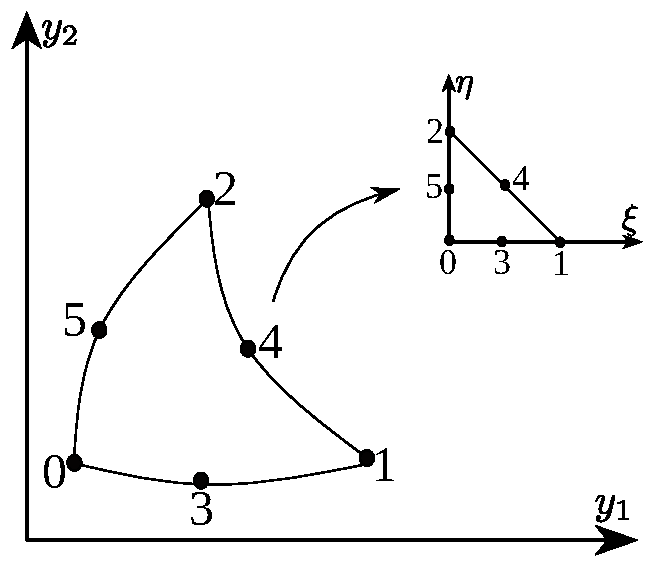
\includegraphics[scale=0.5,trim=0cm 0cm 0cm 0cm, clip=true]{Imagens/Cap2/elementoFinito2d.pdf}}\\
	\subfloat[Elemento Finito 3d\label{fig:elementoFinito3d}]{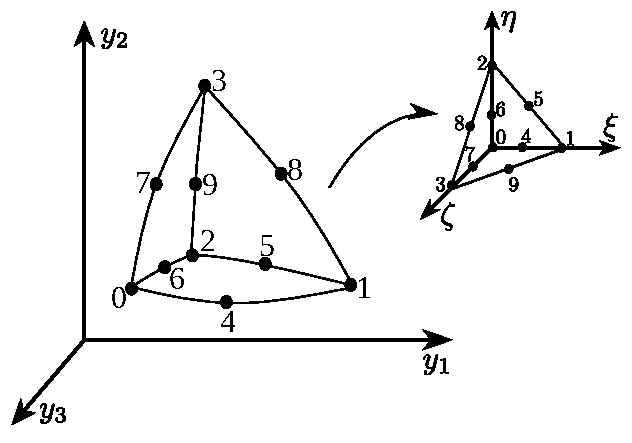
\includegraphics[trim=0 0 0 0,clip,scale=0.65]{Imagens/Cap2/elementoFinito3d.pdf}}
	\caption{Elementos Finitos: representação espacial e paramétrica}
\end{figure}

Adotar a abordagem isoparamétrica implica que a geometria do problema é descrita também pela combinação entre funções de forma e as coordenadas nodais da malha, conforme equação abaixo:

\begin{align}
	\pos^{h} = \sum_{A = 1}^{\nnos} \pos_{A}\shapef_{A}(\pos),  \label{eq:interp_geo}
\end{align}

\noindent sendo que para uma geometria tridimensional o vetor $\pos$ possui coordenadas $y_1,y_2$ e $y_3$, as quais representam as posições físicas do domínio; O subíndice "$A$" $ \ $ representa o índice dos nós da malha, $\nnos$ o número total de nós e $\shapef$ as funções de forma da discretização.

A discretização das variáveis de interesse para DFC no contexto do método dos elementos finitos serão apresentados no seguinte capítulo (Cap. \ref{capitulo:Cap2:DiscEspacial}).


\subsection{Discretização Espacial} \label{capitulo:Cap2:DiscEspacial}

Os espaços de função tentativa para velocidade e pressão, bem como as funções teste, no contexto dos método dos elementos finitos, são dados pela combinação linear de parâmetros nodais com funções de forma definidas sobre cada subdomínio, atendendo à partição da unidade, de forma que o problema da dinâmica dos fluidos fica definido como: encontrar $\velocityh \in \usolutionh$ e $\pressh \in \psolutionh$, de tal modo que $\forall$ $\utesth \in \uweightingh$ e $\ptesth \in \pweightingh$ a seguinte expressão seja verdadeira:

\begin{align}
	\begin{split}
		&\int_{\domain} \utesth \cdot \density \left(\left. \frac{\partial\velocityh}{\partial t} \right|_{\posALE} + \left(\velocityh - \velocityALEh \right)\cdot\gradient \velocityh - \sbodyforceh \right) \deriv \domain + \int_{\domain} \straintensor(\utesth) : \stressTensor\left(\velocityh,\pressh \right)  \deriv \domain\\ & - \int_{\boundaryN} \utesth \cdot \surfaceLoadh \deriv \boundaryN \ + \int_{\domain} \ptesth \left(\divergence \cdot \velocityh\right) d \domain = 0,  \label{eq:QM_C_forma_fraca_1} 
	\end{split}
\end{align}

\noindent onde:

\begin{align}
\velocityh(\pos,t) = \sum_{A = 1}^{\nnos} \velocity_{A}(t)\shapef_{A}(\pos), \label{eq:interp_vel}
\end{align}

\begin{align}
\pressh(\pos,t)  = \sum_{A = 1}^{\nnos} \press_{A}(t)\shapef_{A}(\pos),\label{eq:interp_press} 
\end{align}

\begin{align}
\utesth(\pos)  = \sum_{A = 1}^{\nnos} \utest_{A}\shapef_{A}(\pos), \label{eq:interp_utest}
\end{align}

\begin{align}
\ptesth(\pos)  = \sum_{A = 1}^{\nnos} \ptest_{A}\shapef_{A}(\pos), \label{eq:inter_ptest} 
\end{align}

\noindent sendo as variáveis $\utest_{A}$ e $\ptest_{A}$ arbitrárias nas aproximações.

No entanto, as formulações obtidas pelo método de Galerkin são conhecidas por apresentarem oscilações espúrias em escoamentos dominados pela convecção. Uma das formas de se lidar com esse problema é a utilização de métodos estabilizados, como \textit{Streamline-Upwind/Petrov-Galerkin} (SUPG) \cite{BrooksH:1982, HughesT:1984}, aplicado nesse trabalho. Essa metodologia consiste em adicionar à equação da quantidade de movimento, o seu resíduo ponderado por $\SUPG \left(\left(\velocityh - \velocityALEh \right) \cdot \gradient \utesth\right)$, onde $\SUPG$ é um parâmetro de estabilização. Do ponto de vista numérico a aplicação de  sobre o termo convectivo da equação da quantidade de movimento dá origem a um termo difusivo adicional, cuja viscosidade tem magnitude $\SUPG$, e é responsável por garantir a estabilidade numérica em problemas com convecção dominante.

Para os problemas de escoamentos incompressíveis aqui analisados, deve-se levar em conta que os campos de velocidade e pressão não podem ser aproximados arbitrariamente, podendo levar à ocorrência de oscilações espúrias no campo de pressão. Para evitar isso, podem ser escolhidos elementos Taylor-Hood que obedeçam, à condição de \textit{Ladyzhenskaya-Babuška-Brezzi} (LBB) \cite{BrezziF:1991,ZienkiewiczTN:2005,StrangF:2008}, ou pode-se recorrer a um método estabilizado. 

Neste trabalho, para estabilização da pressão, emprega-se a técnica \textit{Pressure Stabilization Petrov Galerkin} (PSPG)   \cite{HughesFB:1986,TezduyarMRS:1992a}. Essa técnica consiste em adicionar à equação da continuidade, o resíduo da equação da quantidade de movimento ponderada pela função $\PSPG \left(\frac{\gradient \ptesth}{\density}\right)$, onde $\PSPG$ é um parâmetro de estabilização. Essa estabilização cria termos dependentes da pressão na equação da continuidade, responsáveis pela flexibilização do campo de pressão e por contornar a condição LBB.

Por fim, para prover maior estabilização em problemas com formação de vórtices, adiciona-se à equação da quantidade de movimento o resíduo da equação da continuidade ponderado por $ \LSIC \density \left(\divergence \cdot \utesth\right)$ \cite{TezduyarO:2000}, sendo $\LSIC$ um parâmetro de estabilização. A estabilização  $\LSIC$ dá origem a um termo do tipo mínimos quadrados, e que também introduz na formulação uma difusão artificial.

Nota-se que a consistência da formulação estabilizada é garantida, uma vez que são adicionados às equações seus resíduos ponderados. Os parâmetros de estabilização $\SUPG$, $\PSPG$ e $\LSIC$ têm função de proporcionar uma solução estável e otimizar a convergência durante o refinamento de malha. A obtenção dos parâmetros estabilizadores será discutida na Subseção \ref{capitulo:Cap2:FormaFraca:taus}. 

Por fim, o problema da dinâmica dos fluidos passa a ser a determinação de $\velocityh \in \usolutionh$ e $\pressh \in \psolutionh$, de tal modo que $\forall$ $\utesth \in \uweightingh$ e $\ptesth \in \pweightingh$ as seguintes expressões sejam verdadeiras:

\begin{align}
\begin{split}
&\int_{\domain} \utesth \cdot \density\left(\left. \frac{\partial\velocityh}{\partial t}\right|_{\posALE}+ \left(\velocityh - \velocityALEh \right) \cdot \gradient \velocityh - \sbodyforceh\right) \deriv \domain +\int_{\domain} \straintensor \left(\utesth\right) : \stressTensor \left(\velocityh,\pressh\right)\ \deriv \domain\\ &
- \int_{\boundaryN}\utesth \cdot \surfaceLoadh \ \deriv \boundaryN 
+ \sum_{e=1}^{\nel} \int_{\domainE} \SUPG \left(\left(\velocityh - \velocityALEh \right) \cdot \gradient \utesth\right) \cdot \resMom\left(\velocityh,\pressh \right)\  \deriv \domain\\
&+ \sum_{e=1}^{\nel} \int_{\domainE} \density \LSIC \divergence \cdot \utesth \resPre\left(\velocityh\right)\  \deriv \domain = 0,
\label{eq:QM_forma_fraca}
\end{split}
\end{align}

\noindent e

\begin{align}
	\begin{split}
	&\int_{\domain}\ptesth \divergence \cdot \velocityh \ \deriv \domain
	+ \sum_{e=1}^{\nel} \int_{\domainE} \PSPG \left(\frac{\gradient \ptesth}{\density}\right) \cdot \resMom\left(\velocityh,\pressh\right) \  \deriv \domain = 0,
	\label{eq:C_forma_fraca}
	\end{split}
	\end{align}

\noindent onde $\resMom$ e $\resPre$ são os resíduos da equação da quantidade de movimento e da equação da continuidade, respectivamente, dados por:

\begin{align}
\resMom\left(\velocityh,\pressh\right)&=\density\left(\left. \frac{\partial\velocityh}{\partial t}\right|_{\posALE}+\left(\velocityh - \velocityALEh \right)\cdot \gradient \velocityh - \sbodyforceh\right) - \divergence \cdot \stressTensor\left(\velocityh,\pressh\right),
\end{align}

\noindent

\begin{align}
\resPre\left(\velocityh\right)&=\divergence \cdot \velocityh.
\end{align}

A solução de modelos móveis requer a utilização de uma técnica adequada para movimentação da malha local. A técnica utilizada nesse trabalho é conhecida como MJBS (Mesh-Jacobian Based Stiffening) introduzida por \citeonline{TezduyarBSJ:1992f} e será abordada na Subseção \ref{capitulo:Cap7:CondAcop:MovMalha}.

Visto que existem funções teste separadas para a velocidade e pressão, pode-se definir dois vetores residuais correspondentes a equação da quantidade de movimento ($\NNSM$) e a equação da continuidade ($\NNSC$). Considerando a arbitrariedade de $\utest_{A}$ e $\ptest_{A}$, têm-se:

\begin{align}
\NNSM  = [\left(\NNSM\right)_{A,i}],
\end{align}

\begin{align}
\NNSC =  [\left(\NNSC\right)_{A}],
\end{align}
	
\noindent com:

\begin{align}
	\begin{split}
	\left(\NNSM\right)_{A,i} =&\int_{\domain} \shapef_{A}\mathbf{e_i} \cdot \density\left(\left. \frac{\partial\velocityh}{\partial t}\right|_{\posALE}+\left(\velocityh - \velocityALEh \right)\cdot \gradient \velocityh - \sbodyforceh\right) \deriv \domain +\int_{\domain} \straintensor \left(\shapef_{A}\mathbf{e_i}\right) : \stressTensor \left(\velocityh,\pressh\right)\ \deriv \domain\\ &
	- \int_{\boundaryN}\shapef_{A}\mathbf{e_i} \cdot \surfaceLoadh \ \deriv \boundaryN 
	+ \sum_{e=1}^{\nel} \int_{\domainE} \SUPG \left(\left(\velocityh - \velocityALEh \right) \cdot \gradient \shapef_{A}\mathbf{e_i}\right) \cdot \resMom\left(\velocityh,\pressh \right)\  \deriv \domain\\
	&+ \sum_{e=1}^{\nel} \int_{\domainE} \density \LSIC \left(\divergence \cdot \shapef_{A}\mathbf{e_i}\right) \resPre\left(\velocityh\right)\  \deriv \domain  ,
	\end{split}
\end{align}

\noindent e:

\begin{align}
	\begin{split}
	\left(\NNSC\right)_{A} = &\int_{\domain} \shapef_{A} \divergence \cdot \velocityh \ \deriv \domain  
	+ \sum_{e=1}^{\nel} \int_{\domainE} \PSPG \left(\frac{\gradient \shapef_{A}}{\density}\right) \cdot \resMom\left(\velocityh,\pressh\right) \  \deriv \domain,
	\end{split}
\end{align}

\noindent com $i=1,2$ para problemas 2D e $i=1,3$ para problemas 3D.
		
Considerando $\Acceleration$, $\Velocity$ e $\Press$ os vetores nodais dos graus de liberdade respectivos a velocidade, aceleração e pressão, pode-se escrever a forma semidiscreta do problema da DFC como: Encontrar $\Acceleration$, $\Velocity$ e $\Press$ de maneira que

\begin{align}
\NNSM(\Acceleration,\Velocity,\Press) = \vzero,\label{eq:resid_semi_discr_QM}
\end{align}

\noindent e

\begin{align}
\NNSC(\Acceleration,\Velocity,\Press) = \vzero. \label{eq:resid_semi_discr_C}
\end{align}



\subsection{Parâmetros de estabilização}\label{capitulo:Cap2:FormaFraca:taus}

Para a utilização da metologia estabilizada da DFC, descrita nesse capítulo, a definição adequada dos parâmetros de estabilização desempenha papel fundamental na precisão e estabilidade numérica.

Desde os primeiros desenvolvimentos relacionados aos métodos estabilizados houve um amadurecimento das expressões de definição dos parâmetros $\tau$, as quais passam a levar em consideração formulações mais robustas, sendo adaptadas tanto para elementos de ordem elevadas, quanto para malhas mais complexas, como as usadas em análise isogeométrica.

Considerando que nesse trabalho dois tipos de aproximações espaciais são utilizadas, uma baseada no FEM e outra baseada em IGA, adotam-se os parâmetros propostos mais recentemente por \citeonline{TakizawaTO:2018}, \citeonline{TakizawaUT:2019},\citeonline{OtoguroTT:2020}, que são adequados para ambas aproximações. 

Para essa opção é necessário definir-se o tensor métrico do elemento no espaço. Com essa finalidade, descreve-se inicialmente a matriz Jacobiana $\matrixQ$, como:

\begin{align}
	\matrixQ&=\left(\frac{\partial\pos}{\partial\coordAdimen}\right),
\end{align}

\noindent com $\coordAdimen$ representando as coordenadas do espaço paramétrico, com componentes $\xi, \eta$ e $\zeta$.

Para que a ordem polinomial seja levada em consideração, ou, outros fatores como a dimensão do elemento no espaço paramétrico, aplica-se à $\matrixQ$, uma matriz de transformação ($\matrixD$), conforme a seguinte expressão:

\begin{align}
	\matrixQhat&=\matrixQ\matrixD^{-1} \label{eq:q_chap}.
\end{align}

O comprimento direcional do elemento fica definido como:

\begin{align}
	\RQD &=2\left(\rRGN\rRGN : \matrixG \right)^{-\frac{1}{2}},
\end{align}

\noindent o fator 2 vem de um típico espaço paramétrico, que é um quadrado ou um cubo com lado de comprimento 2. $\rRGN$ é o vetor unitário na direção do gradiente da intensidade da velocidade e $\matrixG$ o tensor métrico do elemento, os quais são representados respectivamente como:

\begin{align}
	\rRGN&=\frac{\gradient \lVert\velocityh - \velocityALEh\rVert}{\lVert \gradient \lVert\velocityh - \velocityALEh\rVert\rVert} \label{eq:rRGN}
\end{align}

\noindent e

\begin{align}
	\matrixG &= \matrixQhat^{-T} \cdot \matrixQhat^{-1}. \label{eq:tensor_metrico}
\end{align}

Para elementos finitos com funções de forma polinomiais de Lagrange de ordens $p_\xi$, $p_\eta$ e $p_\zeta$ nas direções paramétricas $\xi$, $\eta$ e $\zeta$, respectivamente, com $\xi, \eta, \zeta \in [-1, 1]$, a matriz $\mathbf{D}$ é definida por:

\begin{align}
	\matrixD&=\begin{bmatrix}
		p_{\xi} & 0 & 0\\
		0 & p_{\eta} & 0 \\
		0 & 0 & p_{\zeta}
	\end{bmatrix}.
\end{align}

Em geral, se escolhe o espaço paramétrico baseado em razões como eficiência da integração numérica ou conveniência de implementação. A maioria das metodologias utilizadas para definir o comprimento do elemento não levam este fator em consideração. Para essa finalidade, em \citeonline{TakizawaUT:2019}, apresenta-se a matriz de transformação ($\matrixD$) como:

\begin{align}
	\matrixD = \frac{\partial{\hat{\coordAdimen}}}{\partial{\coordAdimen}},
\end{align}

\noindent com $\hat{\coordAdimen}$ chamado de espaço de paramétrico de preferência.

Para elementos simplex, buscando encontrar uma expressão que leve a um comprimento de elemento que não possua variação em função da ordenação dos nós, os autores introduziram um espaço paramétrico preferido que consiste em um elemento simplex regular com distância entre vértices de 2, e chegaram a seguinte expressão para $\matrixD$ quando $\nsd = 2$:

\begin{align}
	\matrixD&= \frac{\sqrt{2}}{2} \begin{bmatrix}
		\sqrt{3} + 1 & \sqrt{3} - 1 \\
		\sqrt{3} - 1 & \sqrt{3} + 1
	\end{bmatrix},
\end{align}

\noindent e para $\nsd = 3$:

\begin{align}
	\matrixD&= \frac{\sqrt{2}}{3} \begin{bmatrix}
		4 & 1 & 1 \\
		1 & 4 & 1 \\
		1 & 1 & 4
	\end{bmatrix}.
\end{align}


A definição da matriz $\matrixD$ para elementos isogeométricos será descrita na Subseção \ref{capitulo:Cap3:RepreGeo:taus2}.

Além disso, nessa metodologia, o comprimento do elemento é limitado pelos mínimos e máximos valores representados abaixo:

\begin{align}
	h_{min} \equiv 2\min_{r}\left((\rRGN\rRGN:\matrixG)^{-\frac{1}{2}} \right), \\
	h_{max} \equiv 2\max_{r}\left((\rRGN\rRGN:\matrixG)^{-\frac{1}{2}} \right),
\end{align}

\noindent que podem ser reescritos como:

\begin{align}
	h_{min} = 2\left(\lambda_{max}\matrixG\right)^{-\frac{1}{2}}, \\
	h_{max} = 2\left(\lambda_{min}\matrixG\right)^{-\frac{1}{2}},
\end{align}

\noindent onde $\lambda_{max}$ e $\lambda_{min}$ representam os máximos e mínimos autovalores da matriz $\matrixG$. 

Por fim, os parâmetros de estabilização são escritos como:

\begin{align}
	\SUPG = \PSPG =\left(\frac{1}{\SUGNi^2} + \frac{1}{\SUGNii^2} + \frac{1}{\SUGNiii^2} \right)^{-\frac{1}{2}},
\end{align}

\begin{align}
	\LSIC = \SUPG \lVert\velocityh - \velocityALEh\rVert^2,
\end{align}

\noindent onde:

\begin{align}
	\SUGNi^{-2} = \left(\velocityh - \velocityALEh \right) \left(\velocityh - \velocityALEh \right) : \matrixG ,
\end{align}

\begin{align}
	\SUGNii&=\frac{\timeStep}{2},
\end{align}

\noindent e

\begin{align}
	\SUGNiii^{-1} = \kviscosity \left(\rRGN_{reg}\rRGN_{reg} : \matrixG + \left(1 - \rRGN_{reg}^2)4h_{min}^{-2} \right)\right) ,
\end{align}

\noindent sendo $\rRGN_{reg}$ definido como:

\begin{align}
	\rRGN_{reg} =\frac{\gradient \lVert\velocityh - \velocityALEh\rVert}{\lVert \gradient \lVert\velocityh - \velocityALEh\rVert\rVert + \varepsilon\left(\lVert \gradient \lVert\velocityh - \velocityALEh\rVert\rVert\right)_0},
\end{align}

\noindent com $\varepsilon$ uma constante pequena e $\left(\lVert \gradient \lVert\velocityh- \velocityALEh\rVert\rVert\right)_0$ um valor de referência. Os termos $\SUGNi$, $\SUGNii$ e $\SUGNiii$ são parâmetros correspondentes aos termos convectivos, inerciais e viscosos, respectivamente.

\section{Integração Temporal}\label{capitulo:Cap2:IntegTemp}

Para a integração temporal das equações governantes, utiliza-se o método $\alpha$-generalizado. Esse método foi proposto inicialmente por \citeonline{ChungH:1993} no contexto da mecânica das estruturas, e foi estendido para o contexto da dinâmica dos fluidos computacional por \citeonline{JansenWH:2000}.

Considerando que o tempo da análise do problema é definido por um intervalo de $[0,\totalTime]$, o qual é particionado em subintervalos $\timeStep_{n} = t_{n+1} - t_{n}$, com $t_{n}$ e $t_{n+1}$ os instantes anterior e atual, respectivamente. A solução do problema consiste em: conhecida a solução nos graus de liberdade nodais ($\Acceleration$, $\Velocity$ e $\Press$) no passo de tempo $n$, encontrar a solução no passo de tempo $n+1$ de forma que:

\begin{align}
\NNSM(\Acceleration_{n+\alpham},\Velocity_{n+\alphaf},\Press_{n+1}) = \vzero, \label{eq:resid_QM_alpha}\\
\NNSC(\Acceleration_{n+\alpham},\Velocity_{n+\alphaf},\Press_{n+1}) = \vzero, \label{eq:resid_cont_alpha}
\end{align}

\noindent com:

\begin{gather}
\Acceleration_{n+\alpham} = \Acceleration_n + \alpham \left( \Acceleration_{n+1} - \Acceleration_n \right), \label{eq:inter_acel}\\
\Velocity_{n+\alphaf} = \Velocity_n + \alphaf \left( \Velocity_{n+1} - \Velocity_n \right), \label{eq:inter_vel}
\end{gather}

\noindent sendo $\Acceleration_{n+\alpham}$ e $\Velocity_{n+\alphaf}$ valores intermediários entre $t_{n}$ e $t_{n+1}$ do vetor aceleração e velocidade. A relação entre os valores nodais de aceleração e velocidade são calculados de acordo com fórmula discreta de Newmark (ver, por exemplo, \cite{Hughes:1976}):

\begin{gather}
\Velocity_{n+1} = \Velocity_n + \timeStep\left(\left(1-\gamma\right)\Acceleration_n + \gamma\Acceleration_{n+1} \right). \label{eq:Newmark}
\end{gather}

Os parâmetros que definem o instante intermediário, no qual as variáveis serão calculadas, são determinados de forma a proporcionarem estabilidade e precisão ao método. Seguindo a metodologia proposta por \citeonline{JansenWH:2000}, uma precisão de segunda ordem é obtida, para casos lineares, desde que: 

\begin{gather}
\gamma = 1/2 + \alpham - \alphaf,\label{eq:gamma}
\end{gather}

\noindent enquanto que a estabilidade do problema é incondicional com:

\begin{gather}
\alpham \ge \alphaf \ge 1/2.
\end{gather}

Para proporcionar a precisão de segunda-ordem de convergência e estabilidade da solução, pode-se calcular o parâmetro $\gamma$ de acordo com Eq. \ref {eq:gamma} e $\alpham$, $\alphaf$, através de \cite{Hughes:2000}:


\begin{gather}
\alpham = \frac{1}{2}\left(\frac{3 - \specRadius}{1+\specRadius}\right)\label{eq:alpha_m}\\
\end{gather}

\noindent e

\begin{gather}
\alphaf = \frac{1}{1+\specRadius}\label{eq:alpha_f}.
\end{gather}

O parâmetro $\specRadius$ é conhecido como raio espectral da matriz de amplificação quando $\timeStep_{n} \rightarrow \infty$. Esse parâmetro controla a dissipação numérica em altas frequências realizada pelo processo de integração e está contido no intervalo de $[0,1]$. Para $\specRadius = 0$ a dissipação é máxima e para $\specRadius = 1$ não há introdução de difusão numérica ao método.

Para a solução do sistema de equações não lineares compostas por Eq. \eqref{eq:resid_QM_alpha} e Eq. \eqref{eq:resid_cont_alpha} utiliza-se o método de Newton-Raphson. O método pode ser separado em duas etapas, uma etapa preditiva e outra iterativa corretiva \cite{BazilevsTT:2013}.

Na etapa preditiva, conhecida a solução em um passo de tempo $n$, prediz-se a solução em $n+1$ com as seguintes equações:

\begin{align}
\Acceleration_{n+1}^{0} = \frac{\gamma-1}{\gamma}\Acceleration_{n} \label{eq:pred_acel},
\end{align}

\begin{align}
\Velocity_{n+1}^{0} = \Velocity_{n}, \label{eq:pred_vel}
\end{align}

\begin{align}
\Press_{n+1}^{0} = \Press_{n},\label{eq:pred_press}
\end{align}

\noindent onde o índice $0$ representa a iteração de número zero. 

Na etapa iterativa corretiva, itera-se sobre a Eq. \eqref{eq:resid_QM_alpha} e Eq. \eqref{eq:resid_cont_alpha} até que elas sejam satisfeitas, considerando uma tolerância prescrita, ou até que se alcance uma quantidade máxima de iterações pré-estabelecida. Essa etapa é composta por três fases. A fase 1 consiste em determinar os valores no instante intermediário para as variáveis nodais na iteração $i$:

\begin{align}
\Acceleration_{n+\alpham}^{i} = \Acceleration_n + \alpham \left( \Acceleration_{n+1}^{i} - \Acceleration_n \right), \label{eq:inter_acel_i}\\
\Velocity_{n+\alphaf}^{i} = \Velocity_n + \alphaf \left( \Velocity_{n+1}^{i} - \Velocity_n \right), \label{eq:inter_vel_i}\\
\Press_{n+1}^{i} = \Press_{n+1}^{i} \label{eq:inter_press_i}.
\end{align}

Na fase 2, com os valores intermediários das variáveis nodais resolve-se o sistema linear resultante da linearização das equações Eq. \eqref{eq:resid_QM_alpha} e Eq. \eqref{eq:resid_cont_alpha} com respeito às variáveis de interesse $\Press_{n+1}$ e $\Acceleration_{n+1}$:

\begin{align}
\left .\frac{\partial\NNSM}{\partial\Acceleration_{n+1}}\right|_{i} \Delta \Acceleration_{n+1}^{i} + \left .\frac{\partial\NNSM}{\partial\Press_{n+1}}\right|_{i} \Delta \Press_{n+1}^{i} = -\NNSM^{i}, \label{eq:eq_lin_QM} \\
\left .\frac{\partial\NNSC}{\partial\Acceleration_{n+1}}\right|_{i} \Delta \Acceleration_{n+1}^{i} + \left .\frac{\partial\NNSC}{\partial\Press_{n+1}}\right|_{i} \Delta \Press_{n+1}^{i} = -\NNSC^{i}.\label{eq:eq_lin_cont}
\end{align}

Por fim, na fase 3 atualiza-se a solução através das seguintes relações:

\begin{align}
\Acceleration_{n+1}^{i+1} = \Acceleration_{n+1}^{i} + \Delta\Acceleration_{n+1}^{i},\label{atu_acel} \\ 
\Velocity_{n+1}^{i+1} = \Velocity_{n+1}^{i} + \gamma \timeStep \Delta\Velocity_{n+1}^{i},\label{atu_vel}\\
\Press_{n+1}^{i+1} = \Press_{n+1}^{i} + \Delta\Press_{n+1}^{i}.\label{atu_press}
\end{align}

Na utilização do método $\alpha$-generalizado as integrais das equações Eq. \eqref{eq:resid_QM_alpha} e Eq. \eqref{eq:resid_cont_alpha} são avaliadas no instante $t = t_{n+\alpha_{f}}$, de forma que:

\begin{align}
\int_{\domain} \left(.\right) \deriv \domain = \int_{\domainALEN} \left(.\right) \deriv \domain,
\end{align}

\noindent e, por consequência:

\begin{align}
\domainALEN = \left\{\posh \  |\  \posh(\posALEh,t_{(n+\alphaf)}) = \alphaf \posh(\posALEh,t_{n+1}) + (1-\alphaf) \posh(\posALEh,t_n)  \right\}.
\end{align}


\section{Implementação Computacional} \label{capitulo:Cap2:DFCComputationalCode}


O Algoritmo que descreve a implementação computacional tanto de problemas utilizando o método dos elementos finitos, quanto para problemas utilizando a análise Isogeométrica, é apresentado no Alg. \ref{alg:fluid}.

\begin{algorithm}
	\caption{Algoritmo para problemas de dinâmica dos fluidos computacional}
	\label{alg:fluid}
	\begin{algorithmic}[1]
		\For {o passo de tempo $0$ até $\totalTime$} 
		\State $i=0$;
		\State Predição da solução: aplicação das Eq. \eqref{eq:pred_acel}, Eq. \eqref{eq:pred_vel} e Eq. \eqref{eq:pred_press};
		\While{($\epsilon$ < tolerância)}
		\State $i$++;
		\State Interpolação das variáveis do problema: aplicação da Eq. \eqref{eq:inter_acel_i}, Eq. \eqref {eq:inter_vel_i} e Eq. \eqref{eq:inter_press_i};
		\State Cálculo do incremento nas variáveis do problema: $\Acceleration_{n+1}$ e $\Press_{n+1}$ de acordo com as Eq. \eqref{eq:eq_lin_QM} e Eq. \eqref{eq:eq_lin_cont};
		\State Atualização da solução: calculadas de acordo com Eq. \eqref{atu_acel}, Eq. \eqref{atu_vel} e Eq. \eqref{atu_press}.
		\State Cálculo do erro:
		\begin{align}
		\epsilon =\left\| \NNSM^i \right\|_{L^2}
		\end{align}
		\EndWhile
		\EndFor
	\end{algorithmic}
\end{algorithm}


\section{Verificação e Aplicações} \label{capitulo:Cap2:VerApl}

Para a verificação dos códigos baseados no método dos elementos finitos, adotam-se 2 exemplos muito populares nas bibliografias: Escoamento sobre um cilindro e o problema da cavidade quadrada, os quais são apresentados na subseções sequentes.

\subsection{Escoamento sobre um cilindro} \label{capitulo:Cap2:VerApl:Cilindo}

O estudo do problema de um escoamento sobre um cilindro 2D teve como principal intuito a análise dos coeficientes aerodinâmicos medidos ao longo do tempo e verificar consequentemente se o modelo é capaz de reproduzir os fenômenos relacionados à formação e desprendimento de vórtices característicos desse problema. Para isso, diferentes números de Reynolds ($\Reynolds$) foram estudados, $\Reynolds = 40$, $\Reynolds = 100$ e $\Reynolds = 1000$, os quais são calculados de acordo com a seguinte equação:

\begin{align}
	\Reynolds = \frac{\density L \lVert\velocinfty\lVert}{\viscosity} = \frac{L \lVert \velocinfty \lVert}{\kviscosity}, \label{eq:Reynolds}
\end{align}

\noindent com $L$ a dimensão característica do problema, sendo nesse caso o diâmetro do cilindro, e $\kviscosity$ a viscosidade cinemática do fluido. 

A geometria e condições de contorno são apresentadas na Fig. \ref{fig:cilindro_geometria}. Como pode-se observar trata-se de um domínio retangular, parametrizado em função do diâmetro do cilindro, com um perfil constante de velocidade na entrada e condição de parede lisa nas paredes superior e inferior. No contorno denominado como \textit{saída}, não se conhece o comportamento do escoamento, desta forma, determina-se sua posição no domínio computacional a uma distância grande o suficiente de maneira a não interferir no comportamento do escoamento. 

Na Fig. \ref{fig:cilindro_malha} pode-se observar a malha não-estruturada de elementos finitos utilizada para esse problema, composta por 9122 elementos triangulares quadráticos e 18508 nós. O problema foi simulado para um velocidade de entrada $u_{\infty} = 1,0$, $\density = 1,0$, $\timeStep = 0,05$, e $\specRadius = 0,5$. 

\begin{figure}[!htb]
	\centering
	\subfloat[Geometria e condições de contorno\label{fig:cilindro_geometria}]{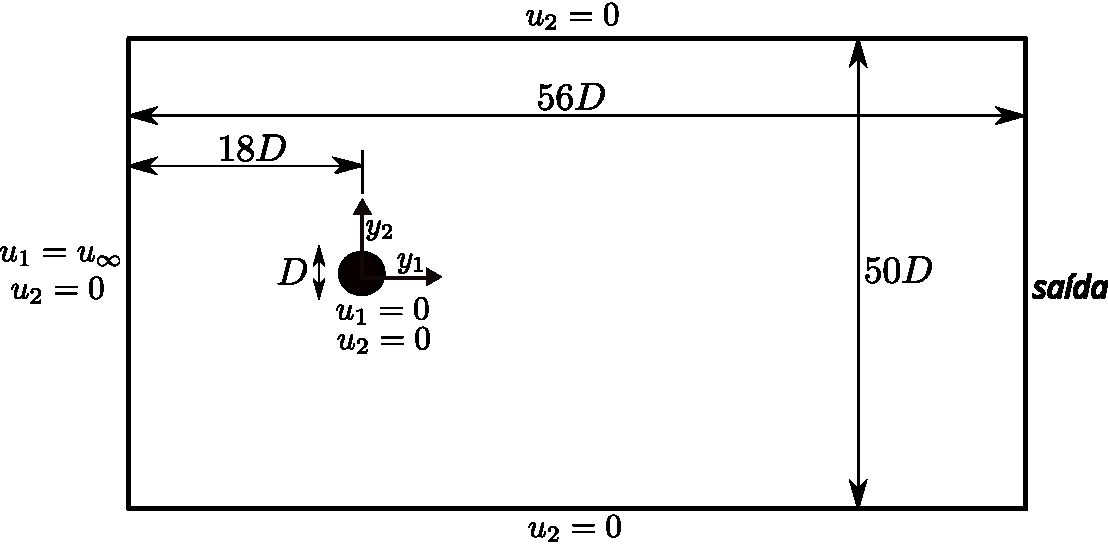
\includegraphics[scale=0.6,trim=0cm 0cm 0cm 0cm, clip=true]{Imagens/Cap2/cilindro_geometria.pdf}}\\
	\subfloat[Discretização espacial\label{fig:cilindro_malha}]{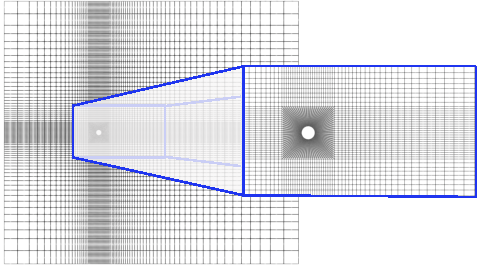
\includegraphics[trim=0cm 2cm 0cm 2cm,clip,scale=0.4]{Imagens/Cap2/cilindro_malha.pdf}}
	\caption{Cilindro: Geometria, condições de contorno e malha de elementos finitos.}
\end{figure}

Para o cálculo dos coeficientes aerodinâmicos é necessário definir-se primeiramente as forças de arrasto - horizontal ($F_D$) e de sustentação - vertical ($F_L$), que são induzidas por tensões desviadores e hidrostáticas e são calculadas pelas seguintes equações:

\begin{align}
F_D = \int_{\boundary_{c}} \stressTensor_{1j}n_{j} \deriv\boundary_{c}, \label{eq:F_D}
\end{align}

\begin{align}
F_L = \int_{\boundary_{c}} \stressTensor_{2j}n_{j} \deriv\boundary_{c},  \label{eq:F_L}
\end{align}

\noindent nas quais o símbolo $\boundary_{c}$ representa o contorno do cilindro e $n_j$ é o vetor normal à esse contorno na direção $j$, com $j=1,2$. Os coeficientes de arrasto e sustentação são definidos respectivamente por:

\begin{align}
	C_D = \frac{F_D}{0,5\density \lVert \velocinfty \lVert^{2} L},
\end{align}

\begin{align}
	C_L = \frac{F_L}{0,5\density \lVert \velocinfty \lVert^{2} L},
\end{align}.

Devido ao fenômeno de desprendimento de vórtices que ocorre a partir de determinado número de Reynolds do escoamento, é usual determinar-se a frequência deste fenômeno através do número adimensional de Strouhal ($\Strouhal$), dado por:

\begin{align}
	\Strouhal = \frac{f_{v}L}{\lVert \velocinfty \lVert},
\end{align}.

\noindent com $f_{v}$ sendo a frequência de desprendimento dos vórtices.

Como pode-se observar na Fig. \ref{fig:cilindro_coefAero} para $\Reynolds = 40$, os coeficientes de arrasto e de sustentação, após o escoamento entrar em fase estacionária, se mantém constantes ao longo de todo o tempo de análise. Isso ocorre, visto que para Reynolds entre 5 à 50, aproximadamente, formam-se dois vórtices simétricos e estacionários na região logo após o cilindro. Posteriormente, o par de vórtices se quebra e passa existir a chamada esteira de Von Karmán, que ocorre devido à formação de vórtices de maneira alternada entre as regiões superior e inferior do cilindro, o que pode ser notado também na Fig. \ref{fig:cilindro_coefAero}  para $\Reynolds = 100$ e $\Reynolds=1000$. Os valores do coeficiente de Strouhal, para $\Reynolds = 100$ e $\Reynolds=1000$, assim como os valores médios obtidos para o coeficiente de arrasto ($C_{Dmed}$) para $\Reynolds = 40$, $\Reynolds = 100$ e $\Reynolds = 1000$ são apresentados na Tab. \ref{tab:cilindro_CD_ST} juntamente com os valores de referência provenientes do trabalho de \citeonline{WANDERLEY2002445}.

\begin{figure}[!htb]
	\centering
	\subfloat[\label{fig:cilindro_Cd}Coeficiente de arrasto $ C_D$]{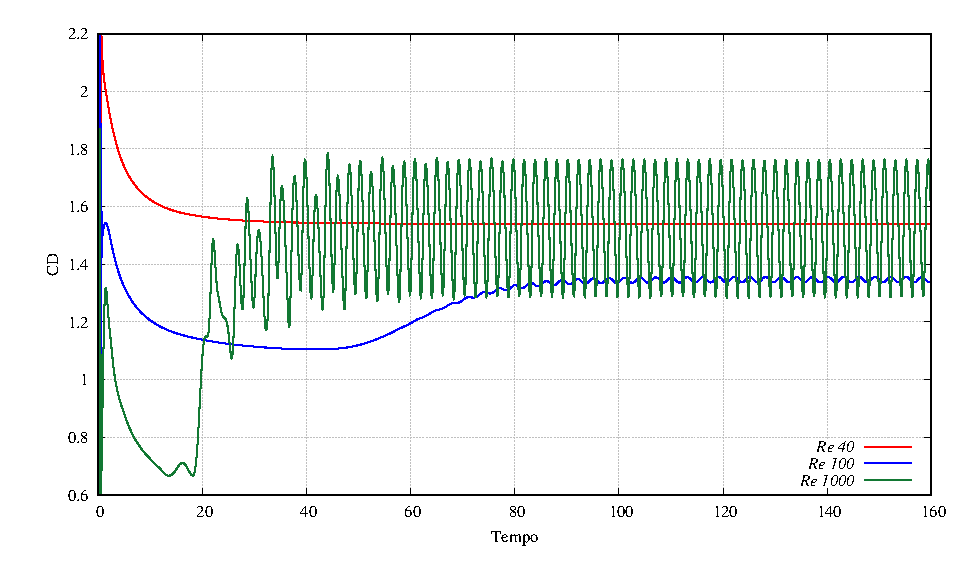
\includegraphics[scale=0.7,trim=0cm 0cm 0cm 0cm, clip=true]{Imagens/Cap2/cilindro_CD.eps}}\\ 
	\subfloat[\label{fig:cilindro_Cl}Coeficiente de sustentação $C_L$]{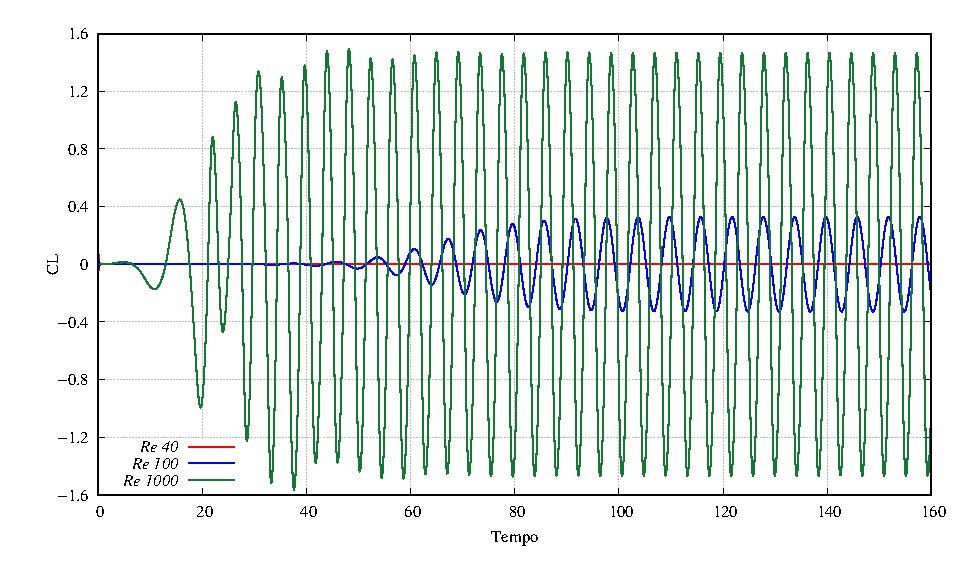
\includegraphics[scale=0.7,trim=0cm 0cm 0cm 0cm, clip=true]{Imagens/Cap2/cilindro_CL.eps}}\\ 
	\caption{Cilindro: Coeficientes aerodinâmicos. }
	\label{fig:cilindro_coefAero}
\end{figure}


\begin{table}[h!]
	\centering
	\caption{Comparação entre valores obtidos e valores de referência para $C_{Dmed}$ e $St$ em diferentes números de Reynolds.}
	\begin{tabular}{|c|c|c|c|c|}
		\hline
		\multirow{2}{*}{$Re$} & \multicolumn{2}{c|}{$C_{Dmed}$} & \multicolumn{2}{c|}{$St$} \\ \cline{2-5}
		& Presente estudo & Referência & Presente estudo & Referência \\ \hline
		40   & 1,54  & 1,59 & - & - \\ \hline
		100  & 1,35 &  1,33 & 0,166 & 0,163 \\ \hline
		1000 & 1,52 &  1,51 & 0,238 & 0,235 \\ \hline
	\end{tabular}
	\label{tab:cilindro_CD_ST}
\end{table}

Nas Fig. \ref{fig:cilindro_camposVel} e Fig. \ref{fig:cilindro_camposPressao} podem ser observados os campos de velocidade e pressão ao longo de um ciclo de desprendimento de vórtices para $\Reynolds = 100$. Pode-se notar nessas imagens, a formação e o desprendimento de vórtices na esteira de Von Karmán.

\begin{figure}[htb!]
	\centering
	\subfloat[$T_n$]{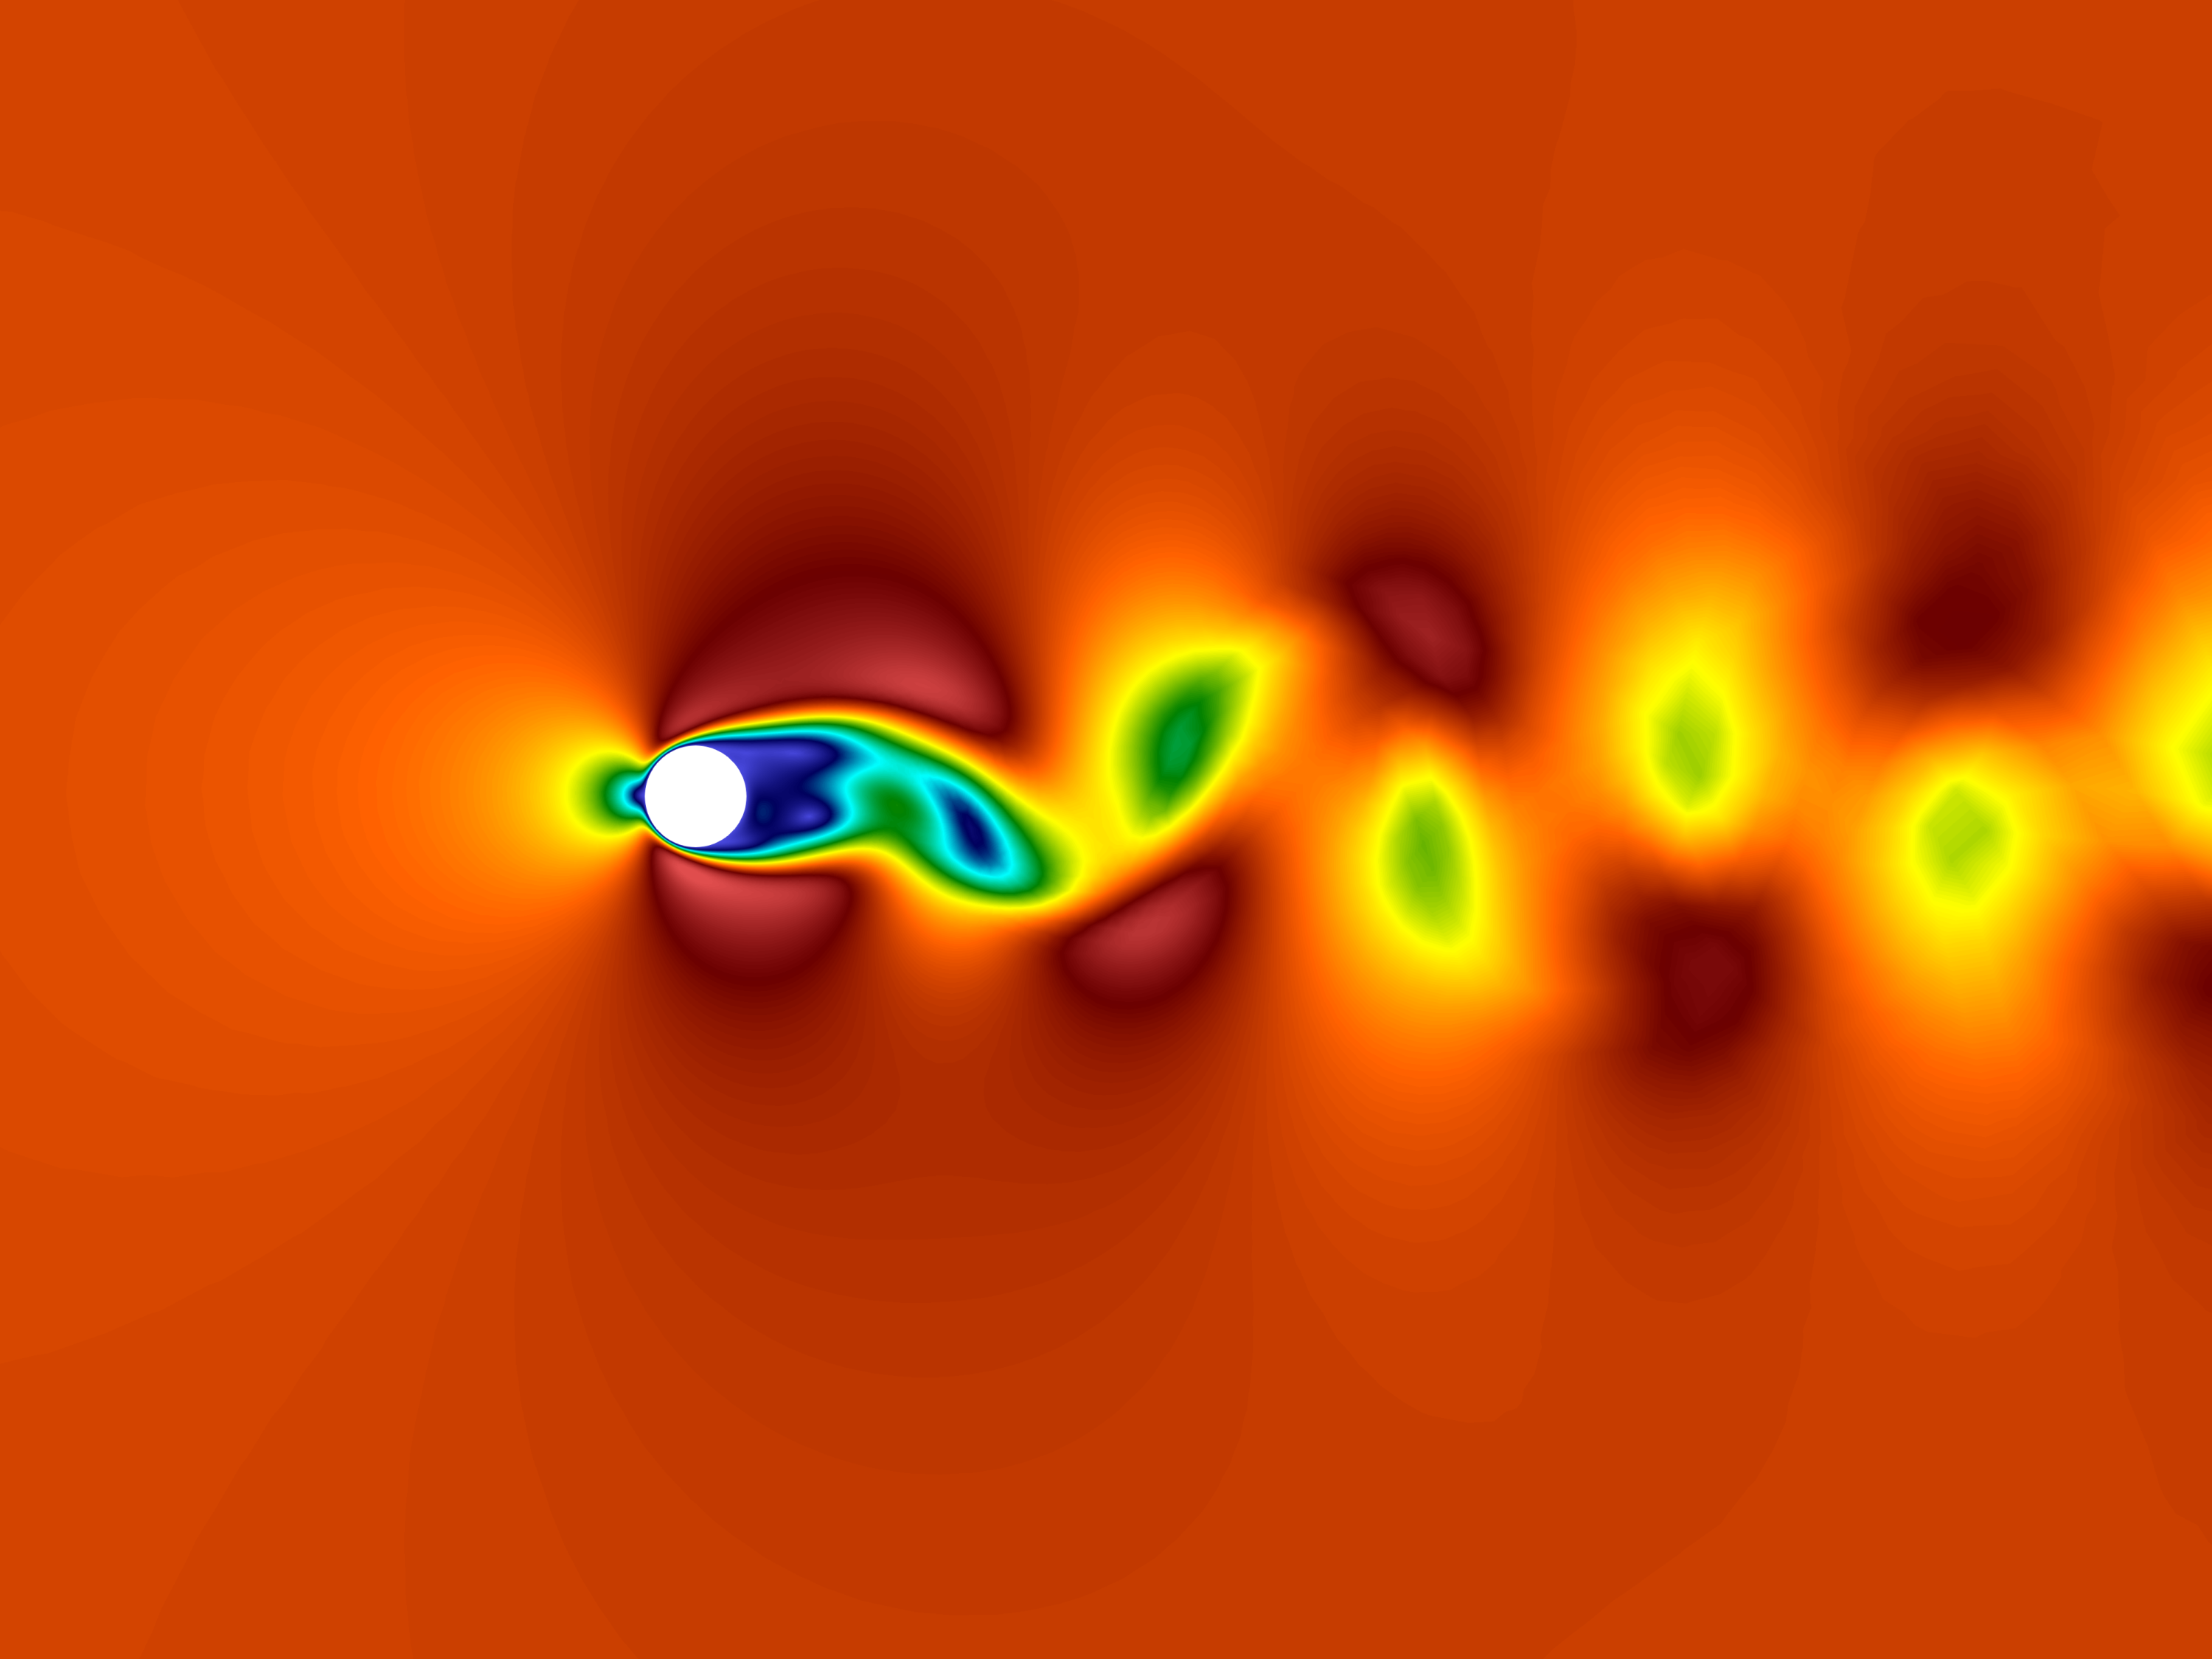
\includegraphics[scale=0.15,trim=5cm 5cm 5cm 6cm, clip=true]{Imagens/Cap2/cilindro_vel2020.pdf}} \
	\subfloat[$T_n + T_n/6$]{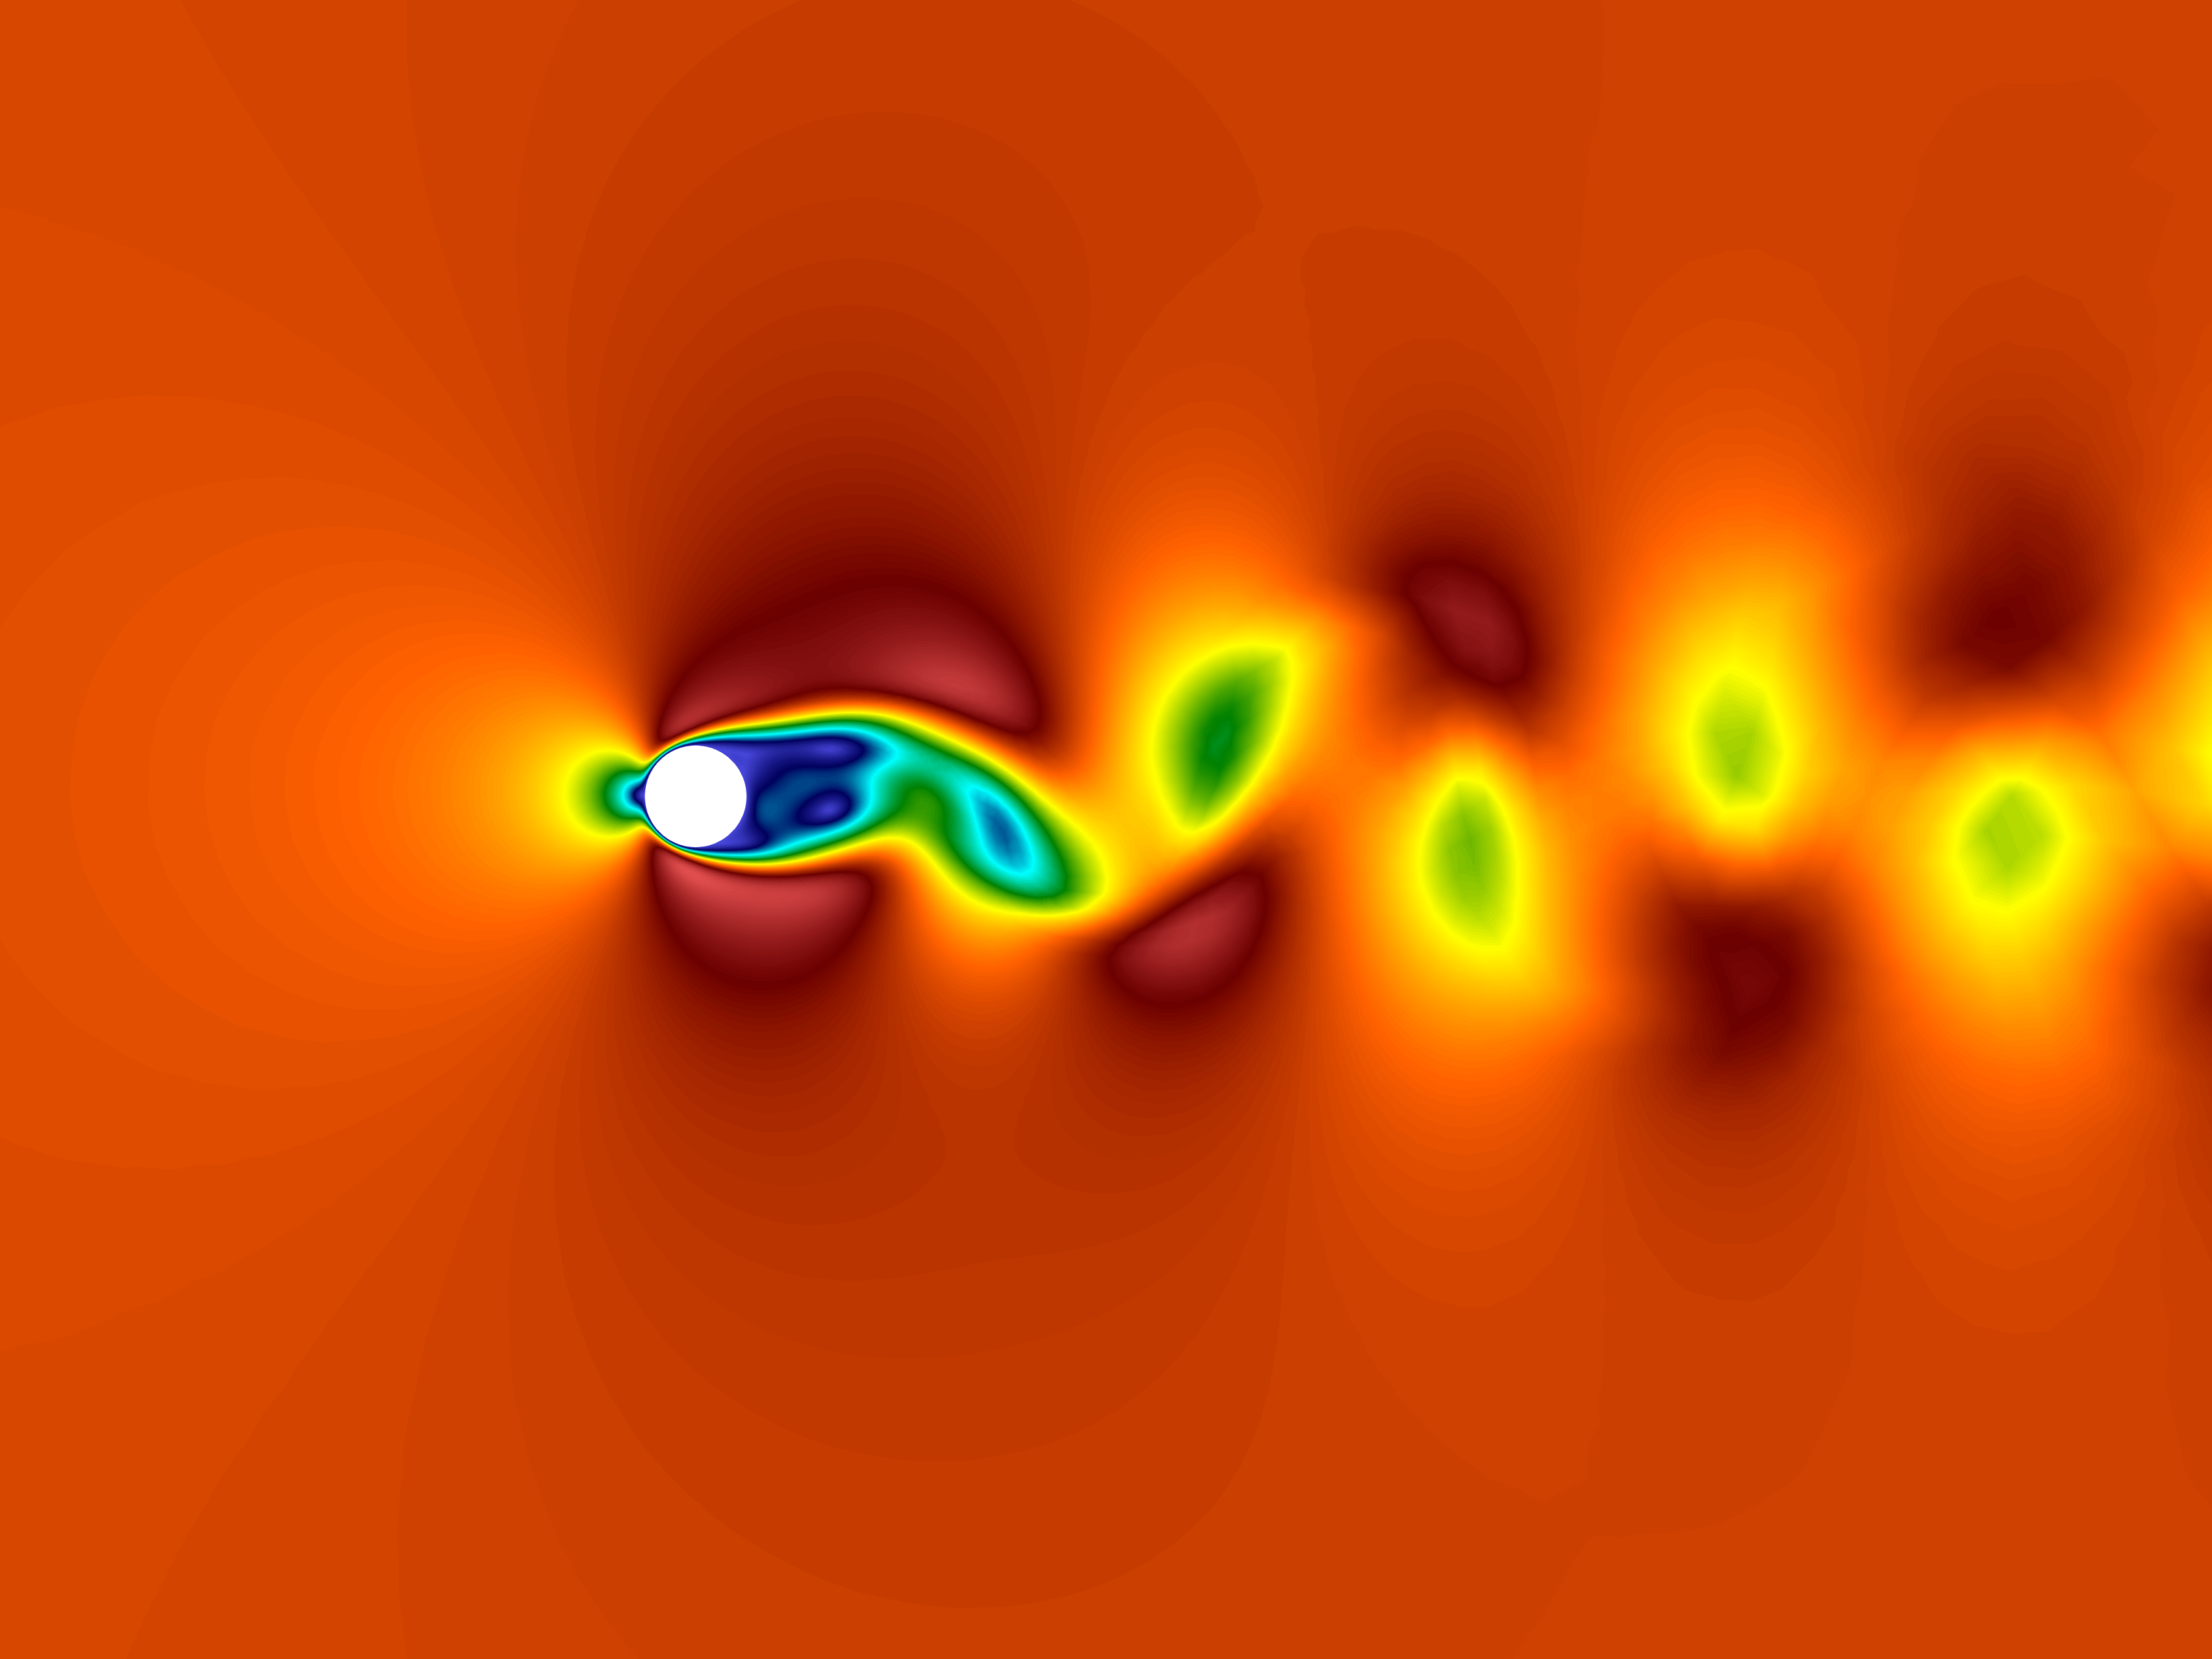
\includegraphics[scale=0.15,trim=5cm 5cm 5cm 6cm, clip=true]{Imagens/Cap2/cilindro_vel2030.pdf}} \\
	\subfloat[$T_n + T_n/3$]{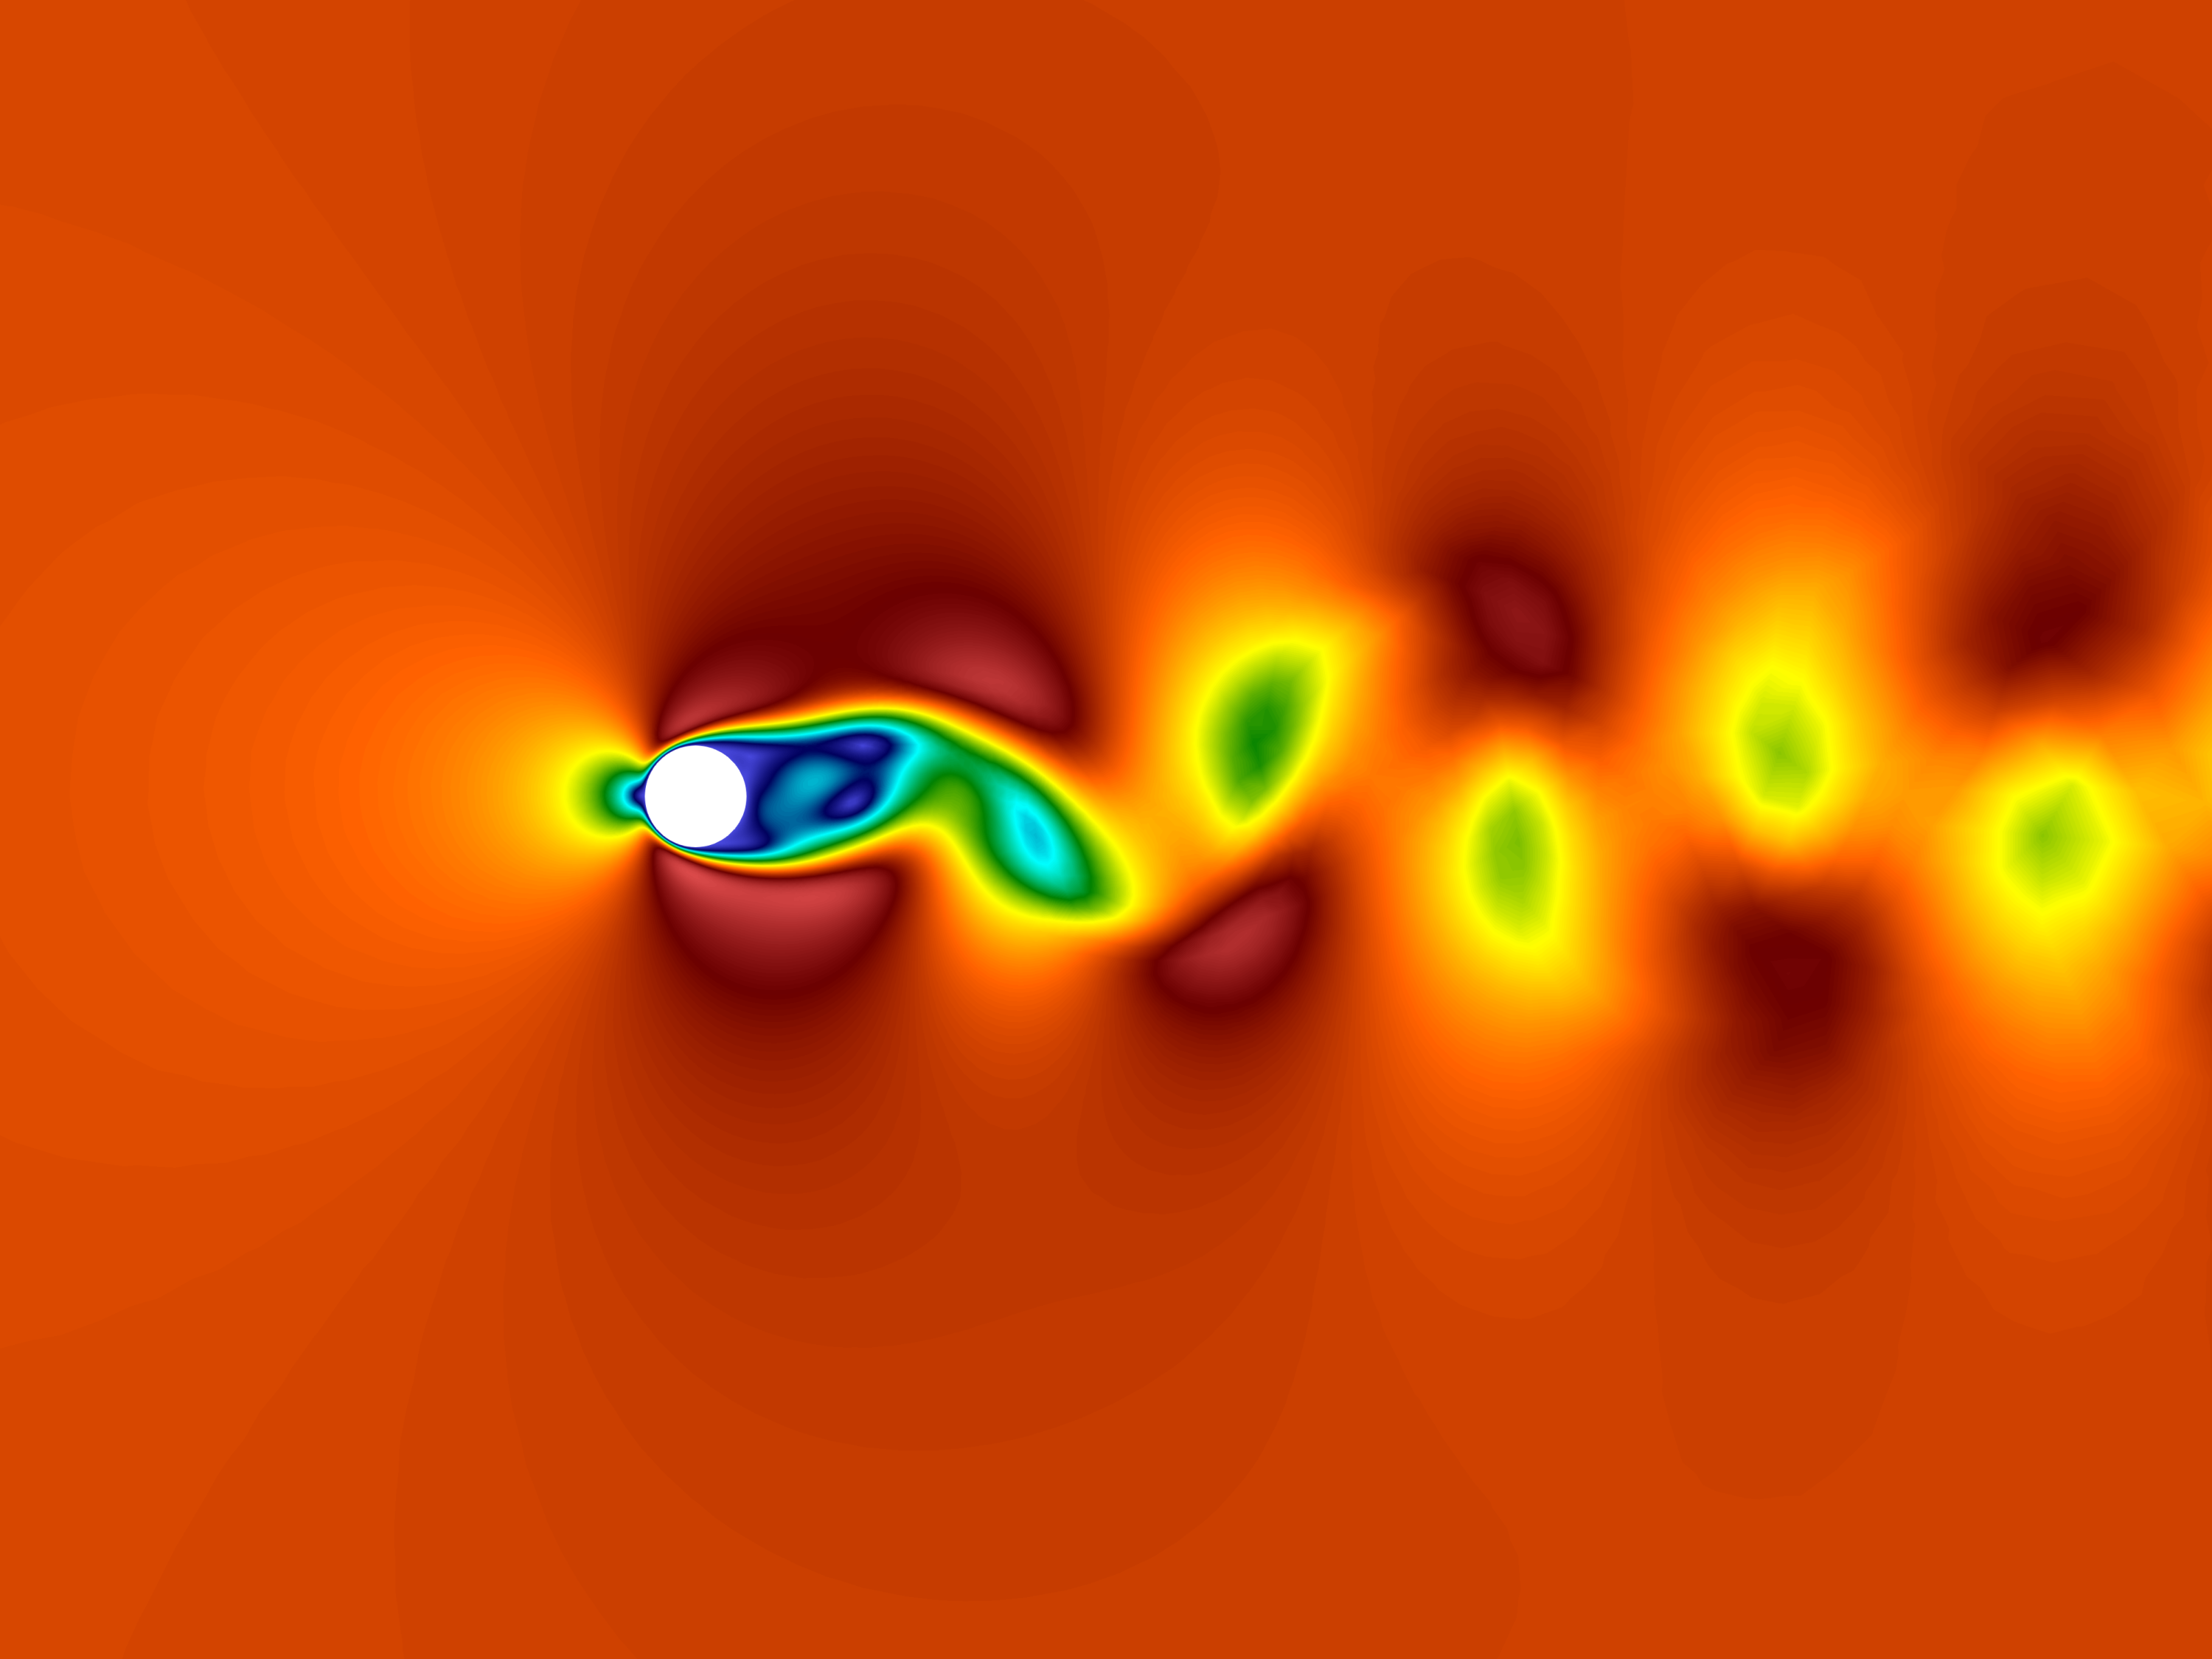
\includegraphics[scale=0.15,trim=5cm 5cm 5cm 6cm, clip=true]{Imagens/Cap2/cilindro_vel2040.pdf}} \
	\subfloat[$T_n + T_n/2$]{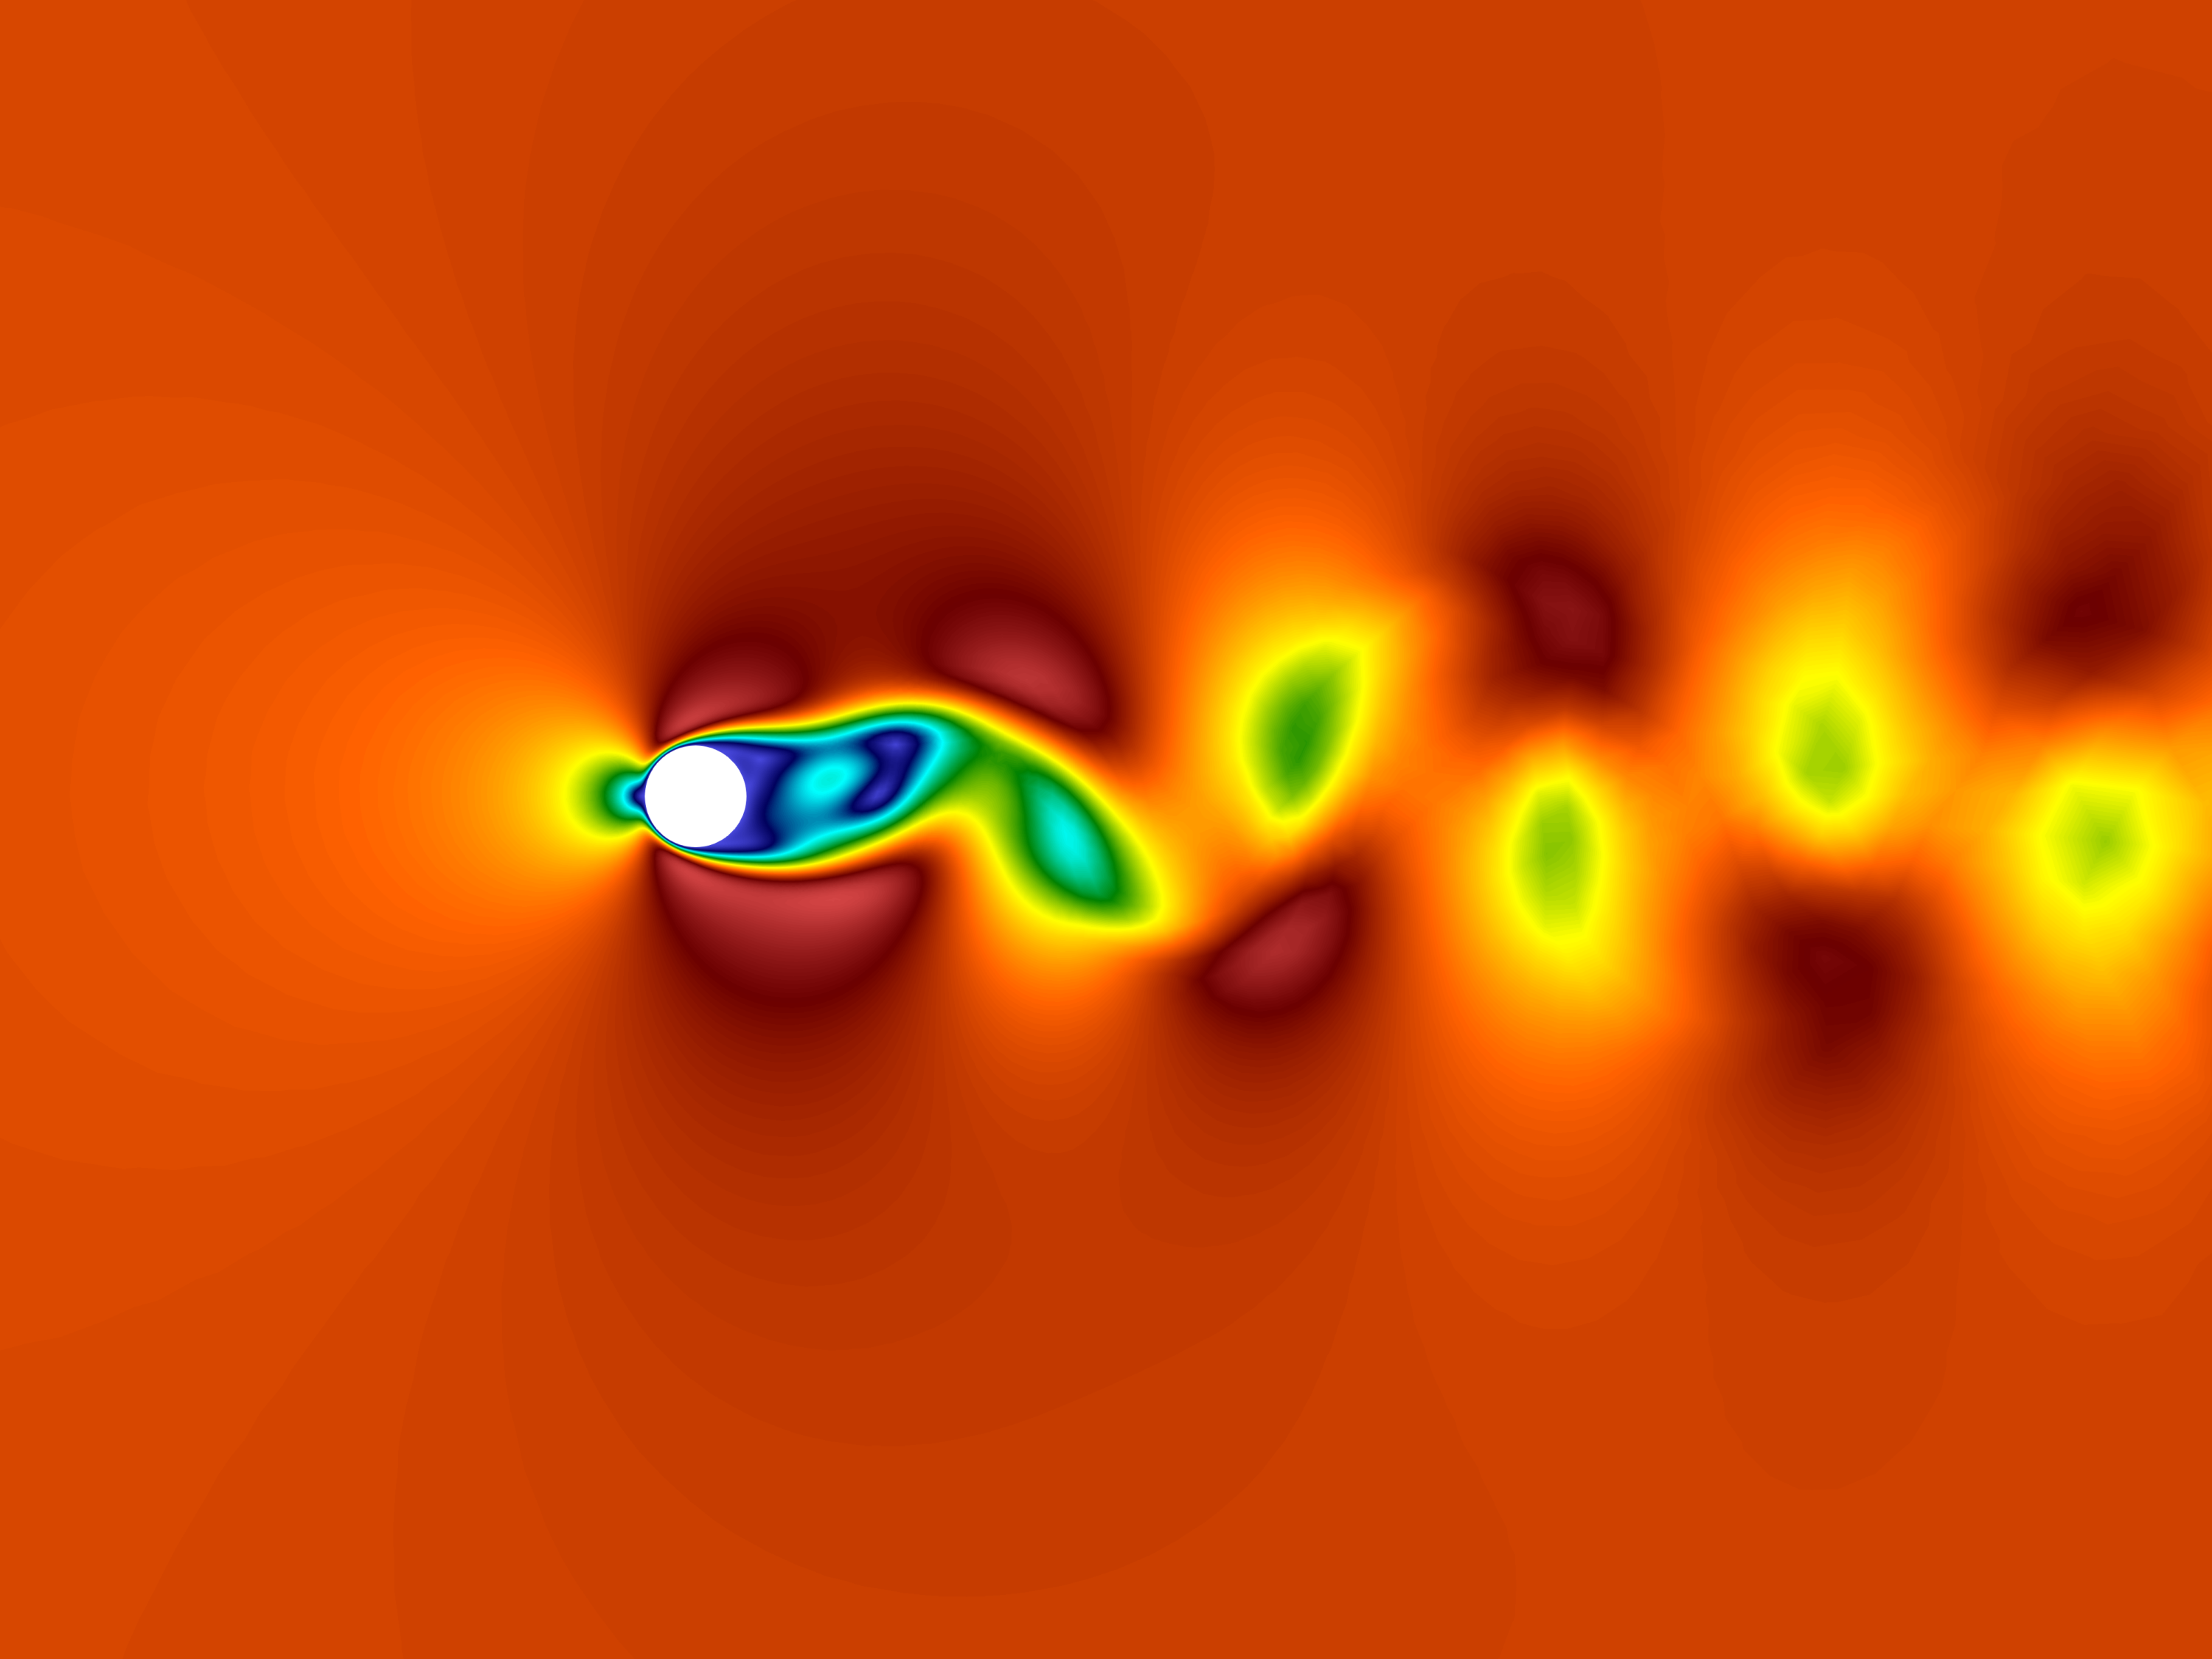
\includegraphics[scale=0.15,trim=5cm 5cm 5cm 6cm, clip=true]{Imagens/Cap2/cilindro_vel2050.pdf}} \\
	\subfloat[$T_n + 2T_n/3$]{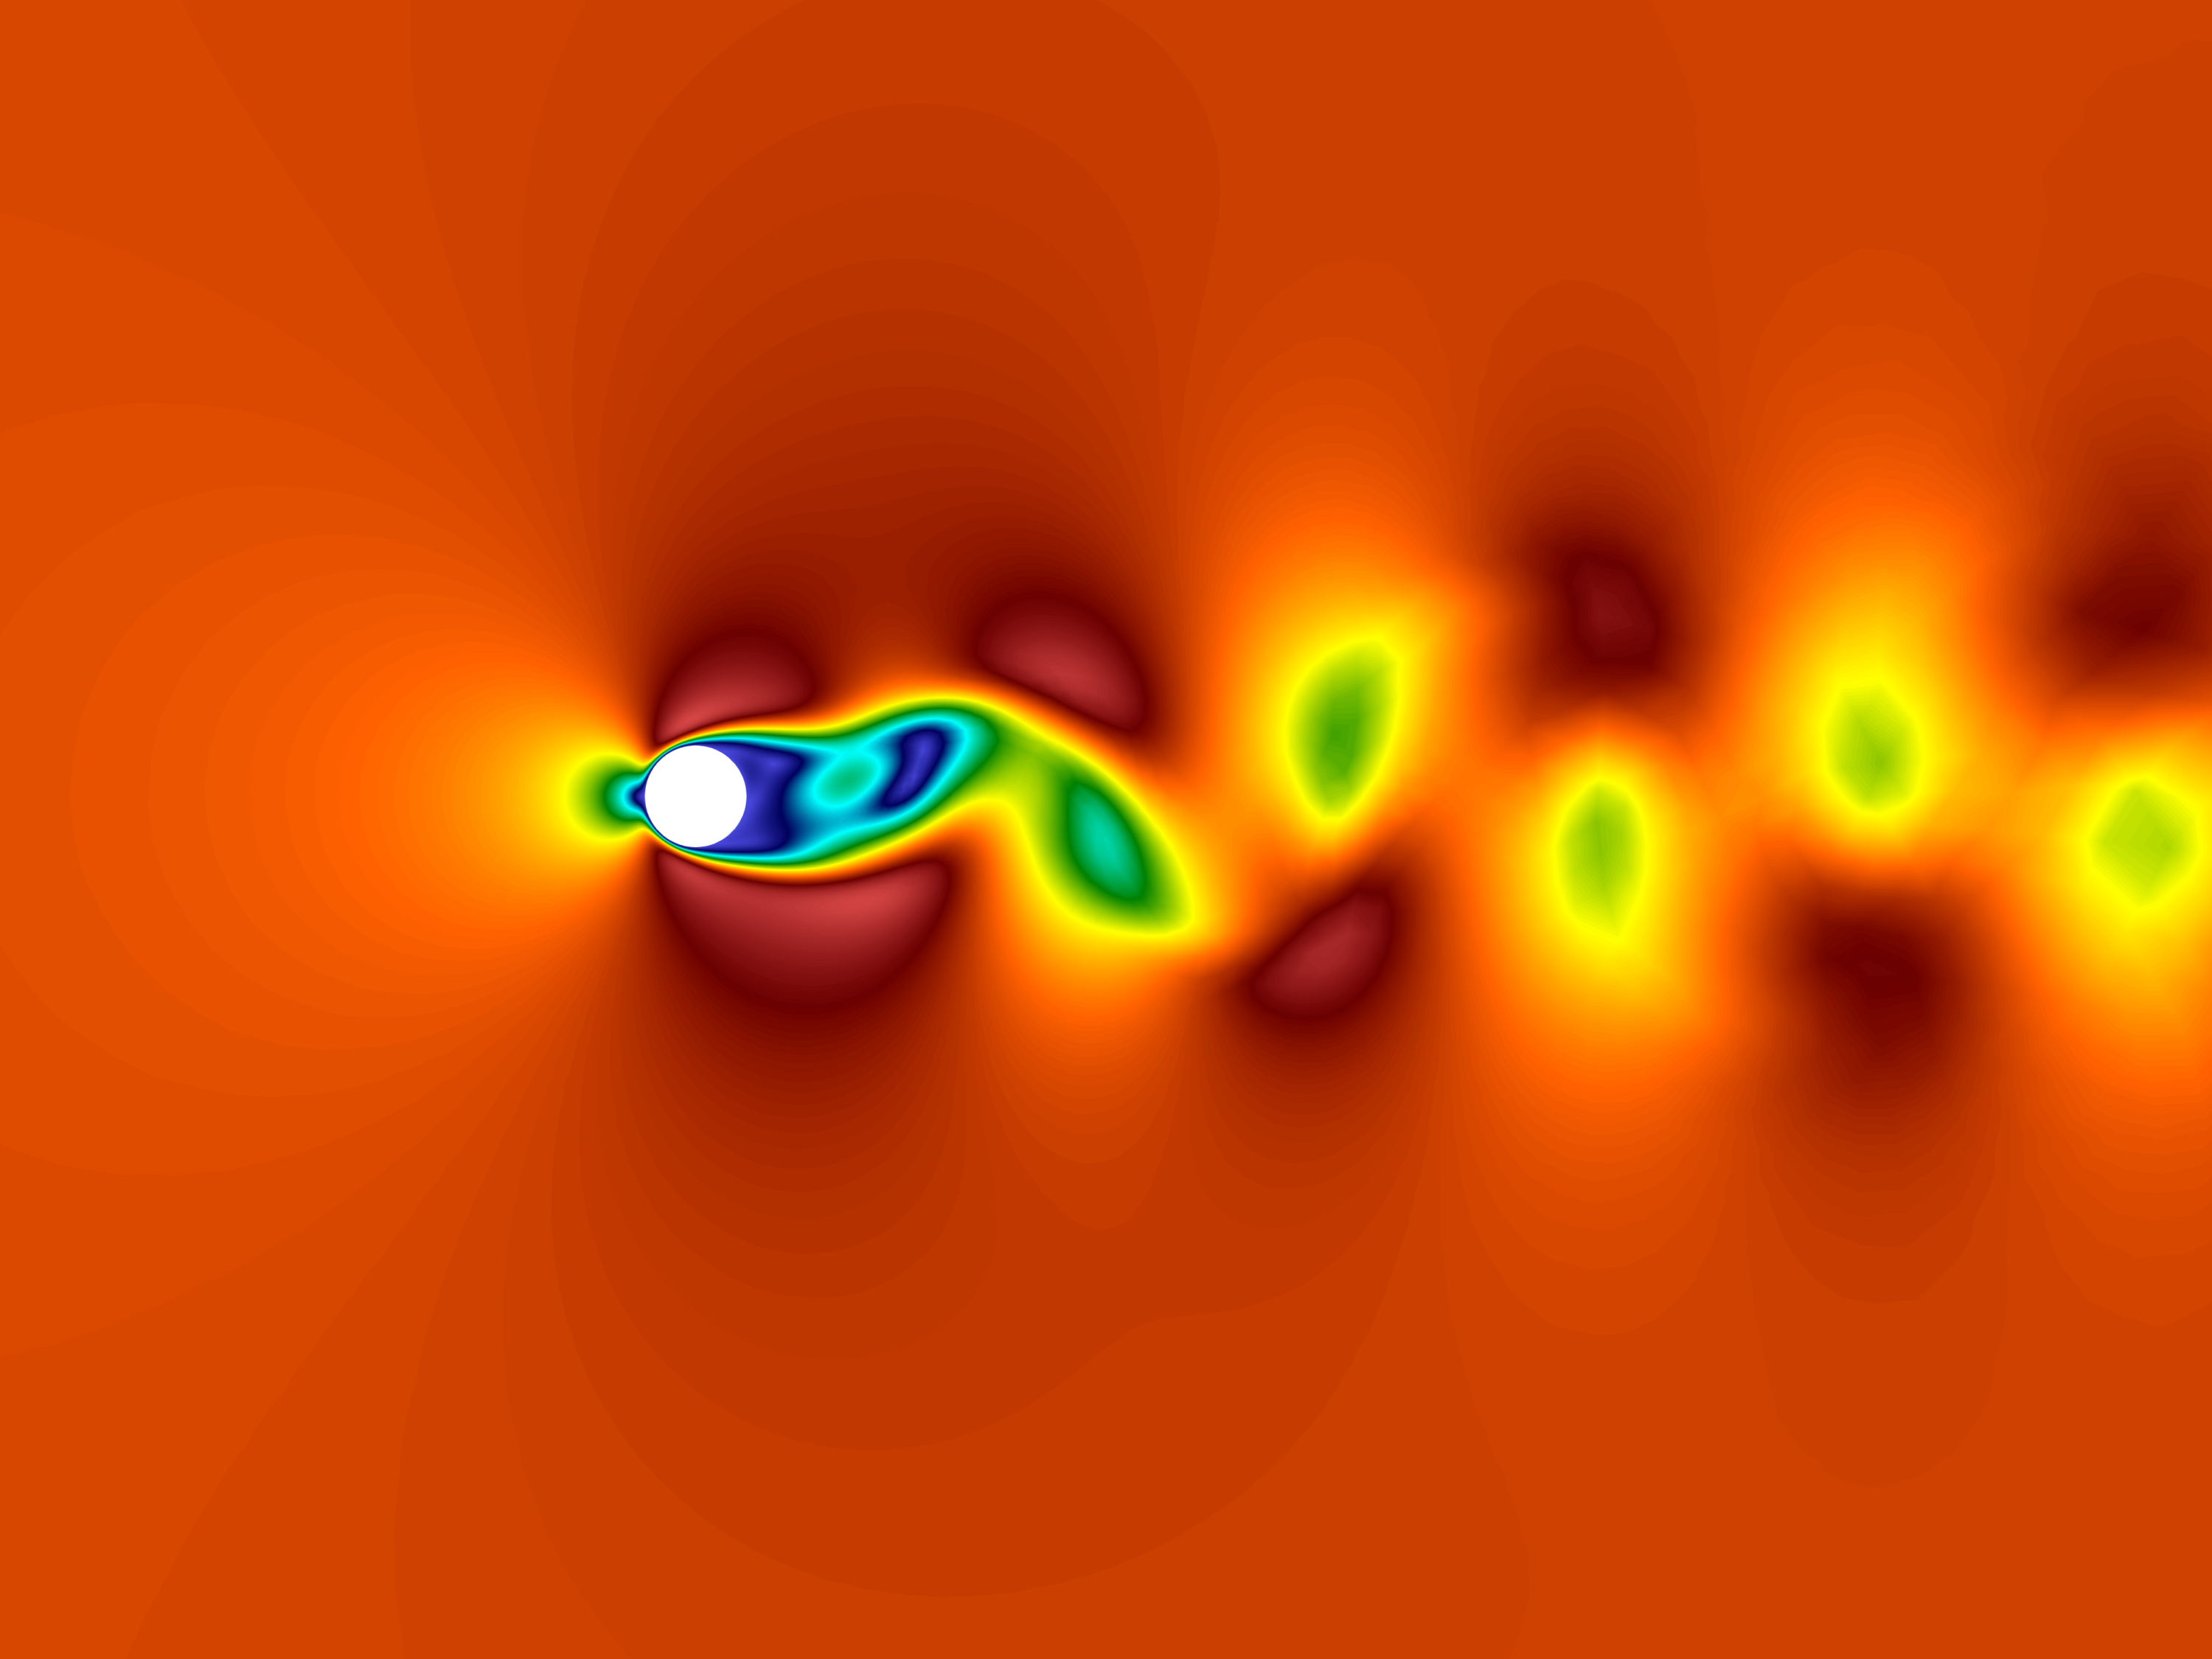
\includegraphics[scale=0.15,trim=5cm 5cm 5cm 6cm, clip=true]{Imagens/Cap2/cilindro_vel2060.pdf}} \
	\subfloat[$T_n + 5T_n/6$]{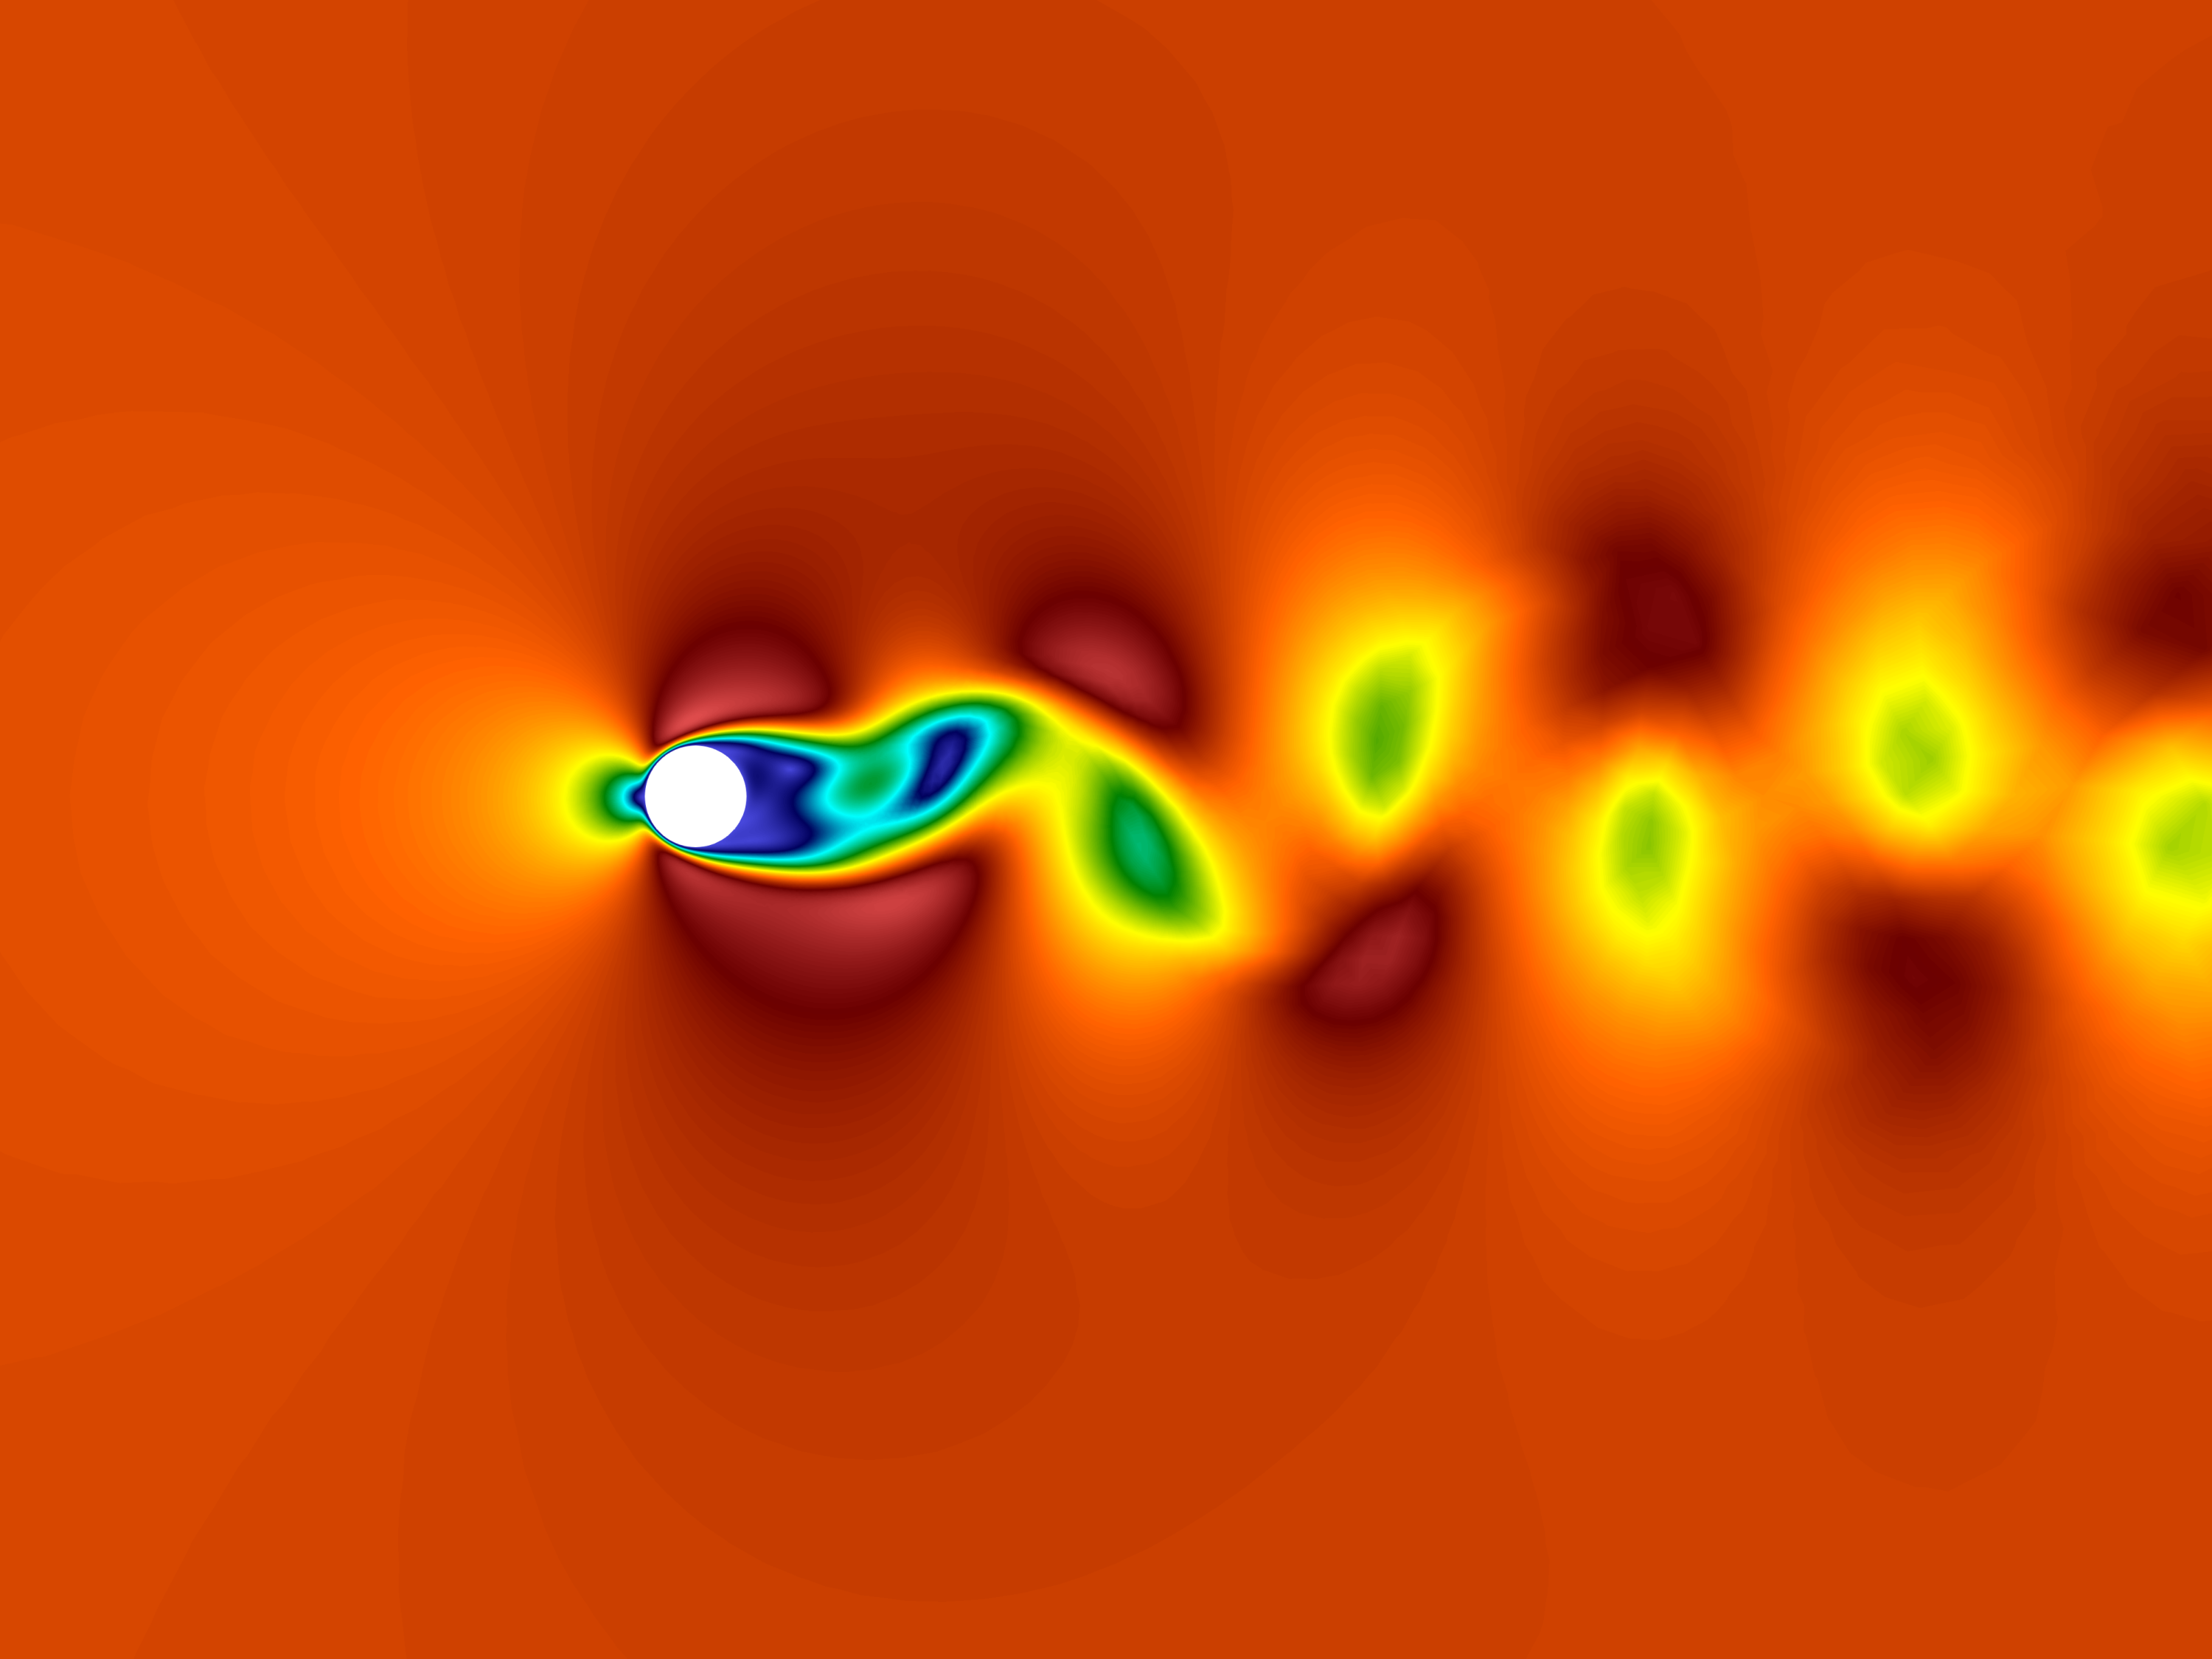
\includegraphics[scale=0.15,trim=5cm 5cm 5cm 6cm, clip=true]{Imagens/Cap2/cilindro_vel2070.pdf}} \\
	{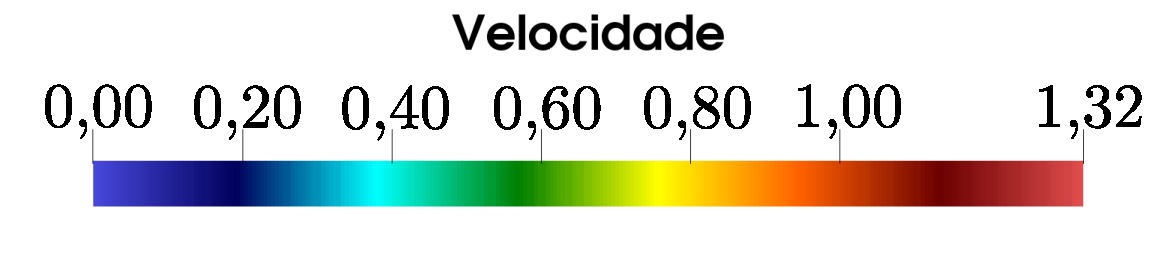
\includegraphics[trim=0cm 0cm 0cm 0cm,clip=true,scale=0.3]{Imagens/Cap2/cilindro_legendaVel.pdf}} \\
	\caption{Cilindro: Campos de velocidade para $\Reynolds = 100$}
	\label{fig:cilindro_camposVel}
\end{figure}

\begin{figure}[htb!]
	\centering
	\subfloat[$T_n$]{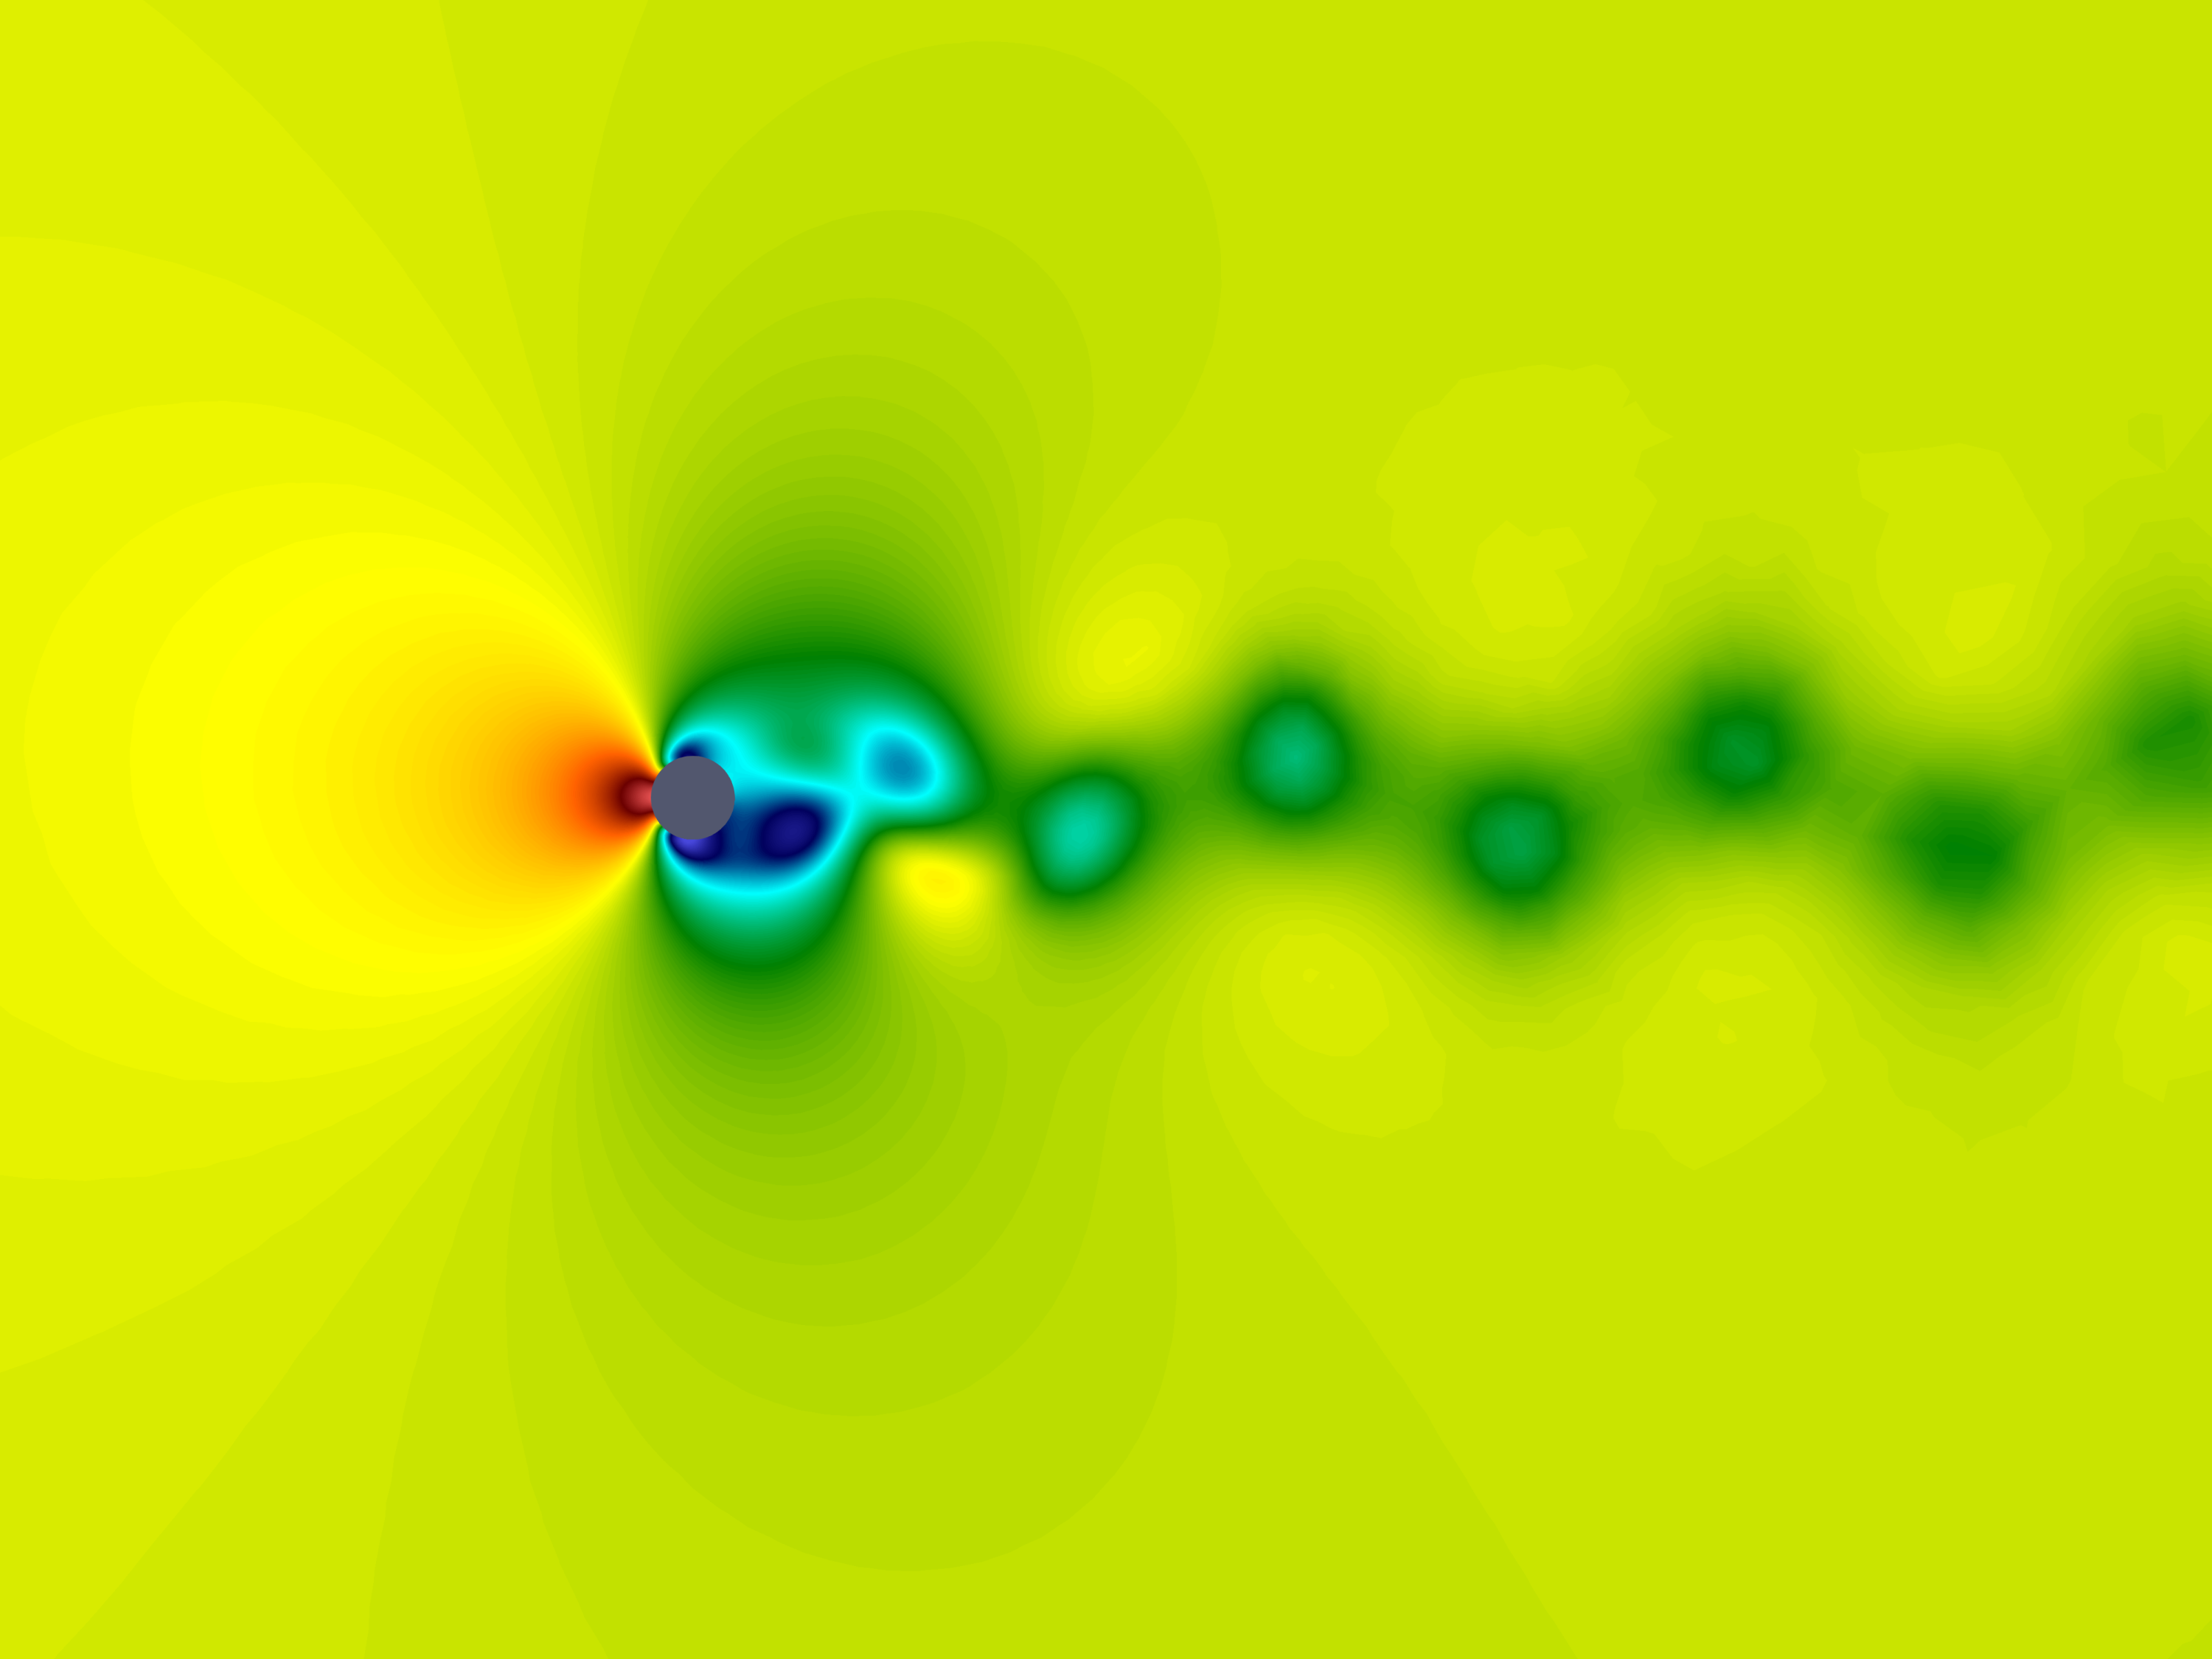
\includegraphics[scale=0.15,trim=5cm 5cm 5cm 6cm, clip=true]{Imagens/Cap2/cilindro_press2020.pdf}} \
	\subfloat[$T_n + T_n/6$]{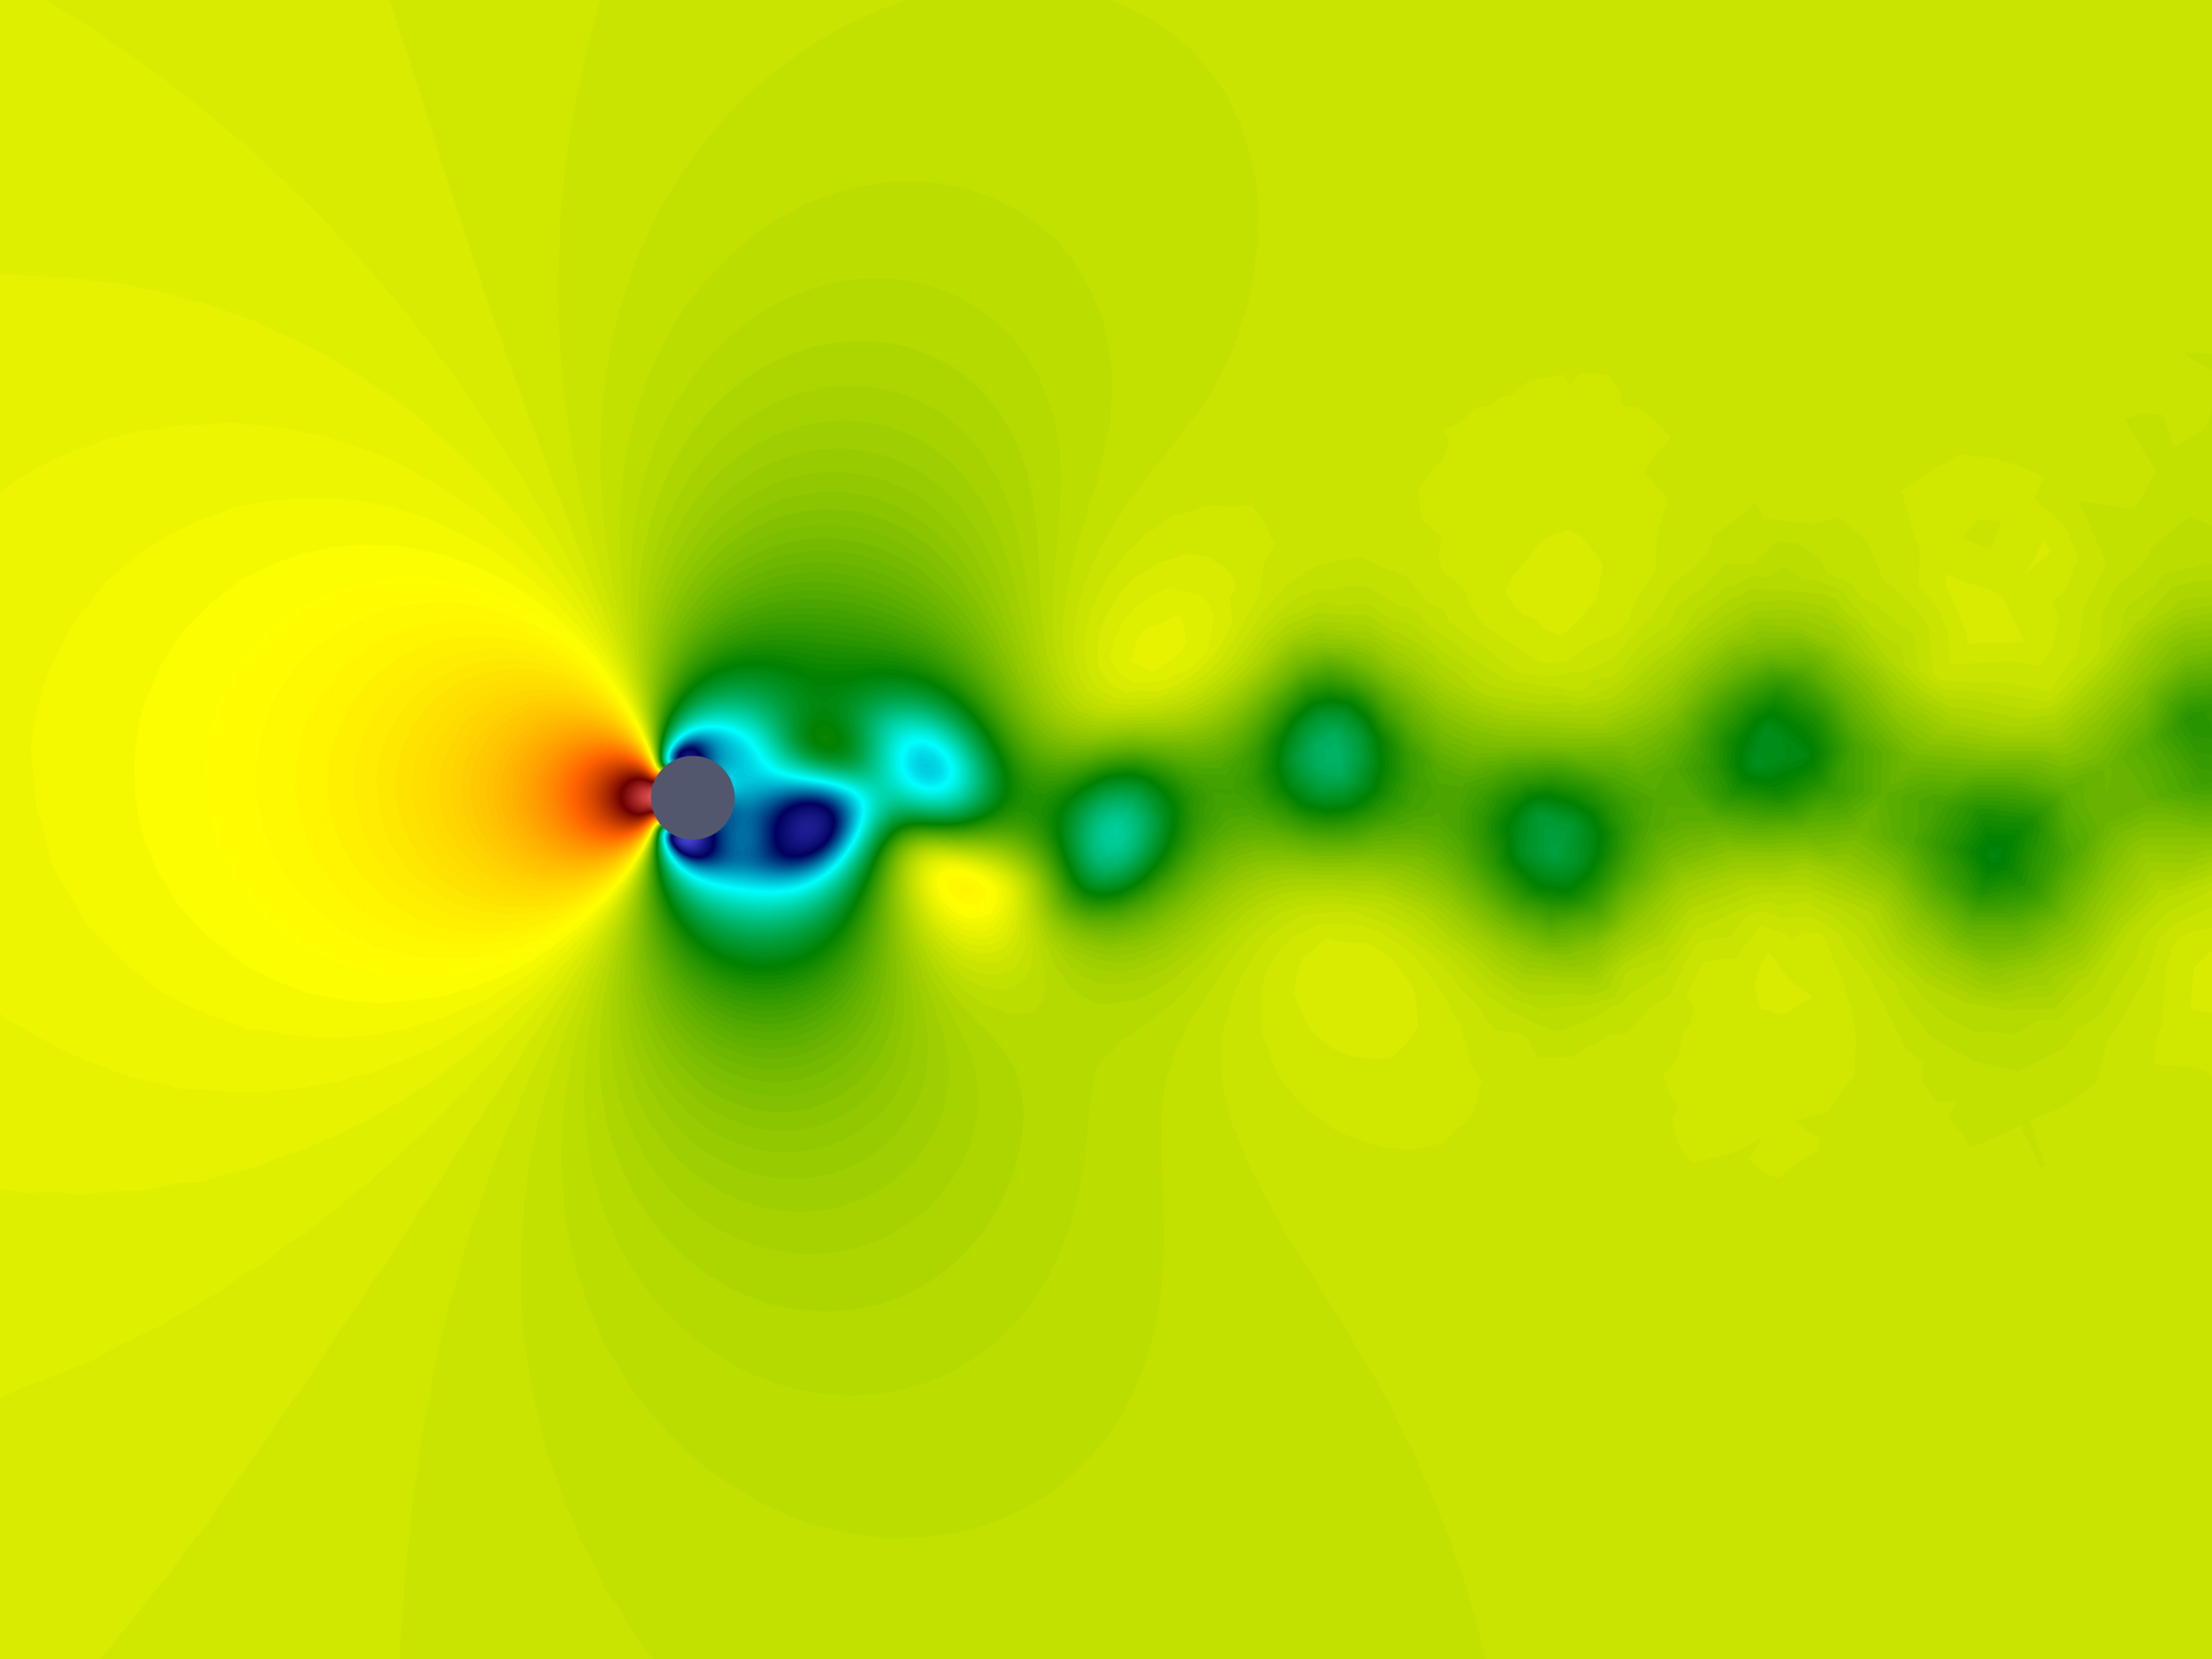
\includegraphics[scale=0.15,trim=5cm 5cm 5cm 6cm, clip=true]{Imagens/Cap2/cilindro_press2030.pdf}} \\
	\subfloat[$T_n + T_n/3$]{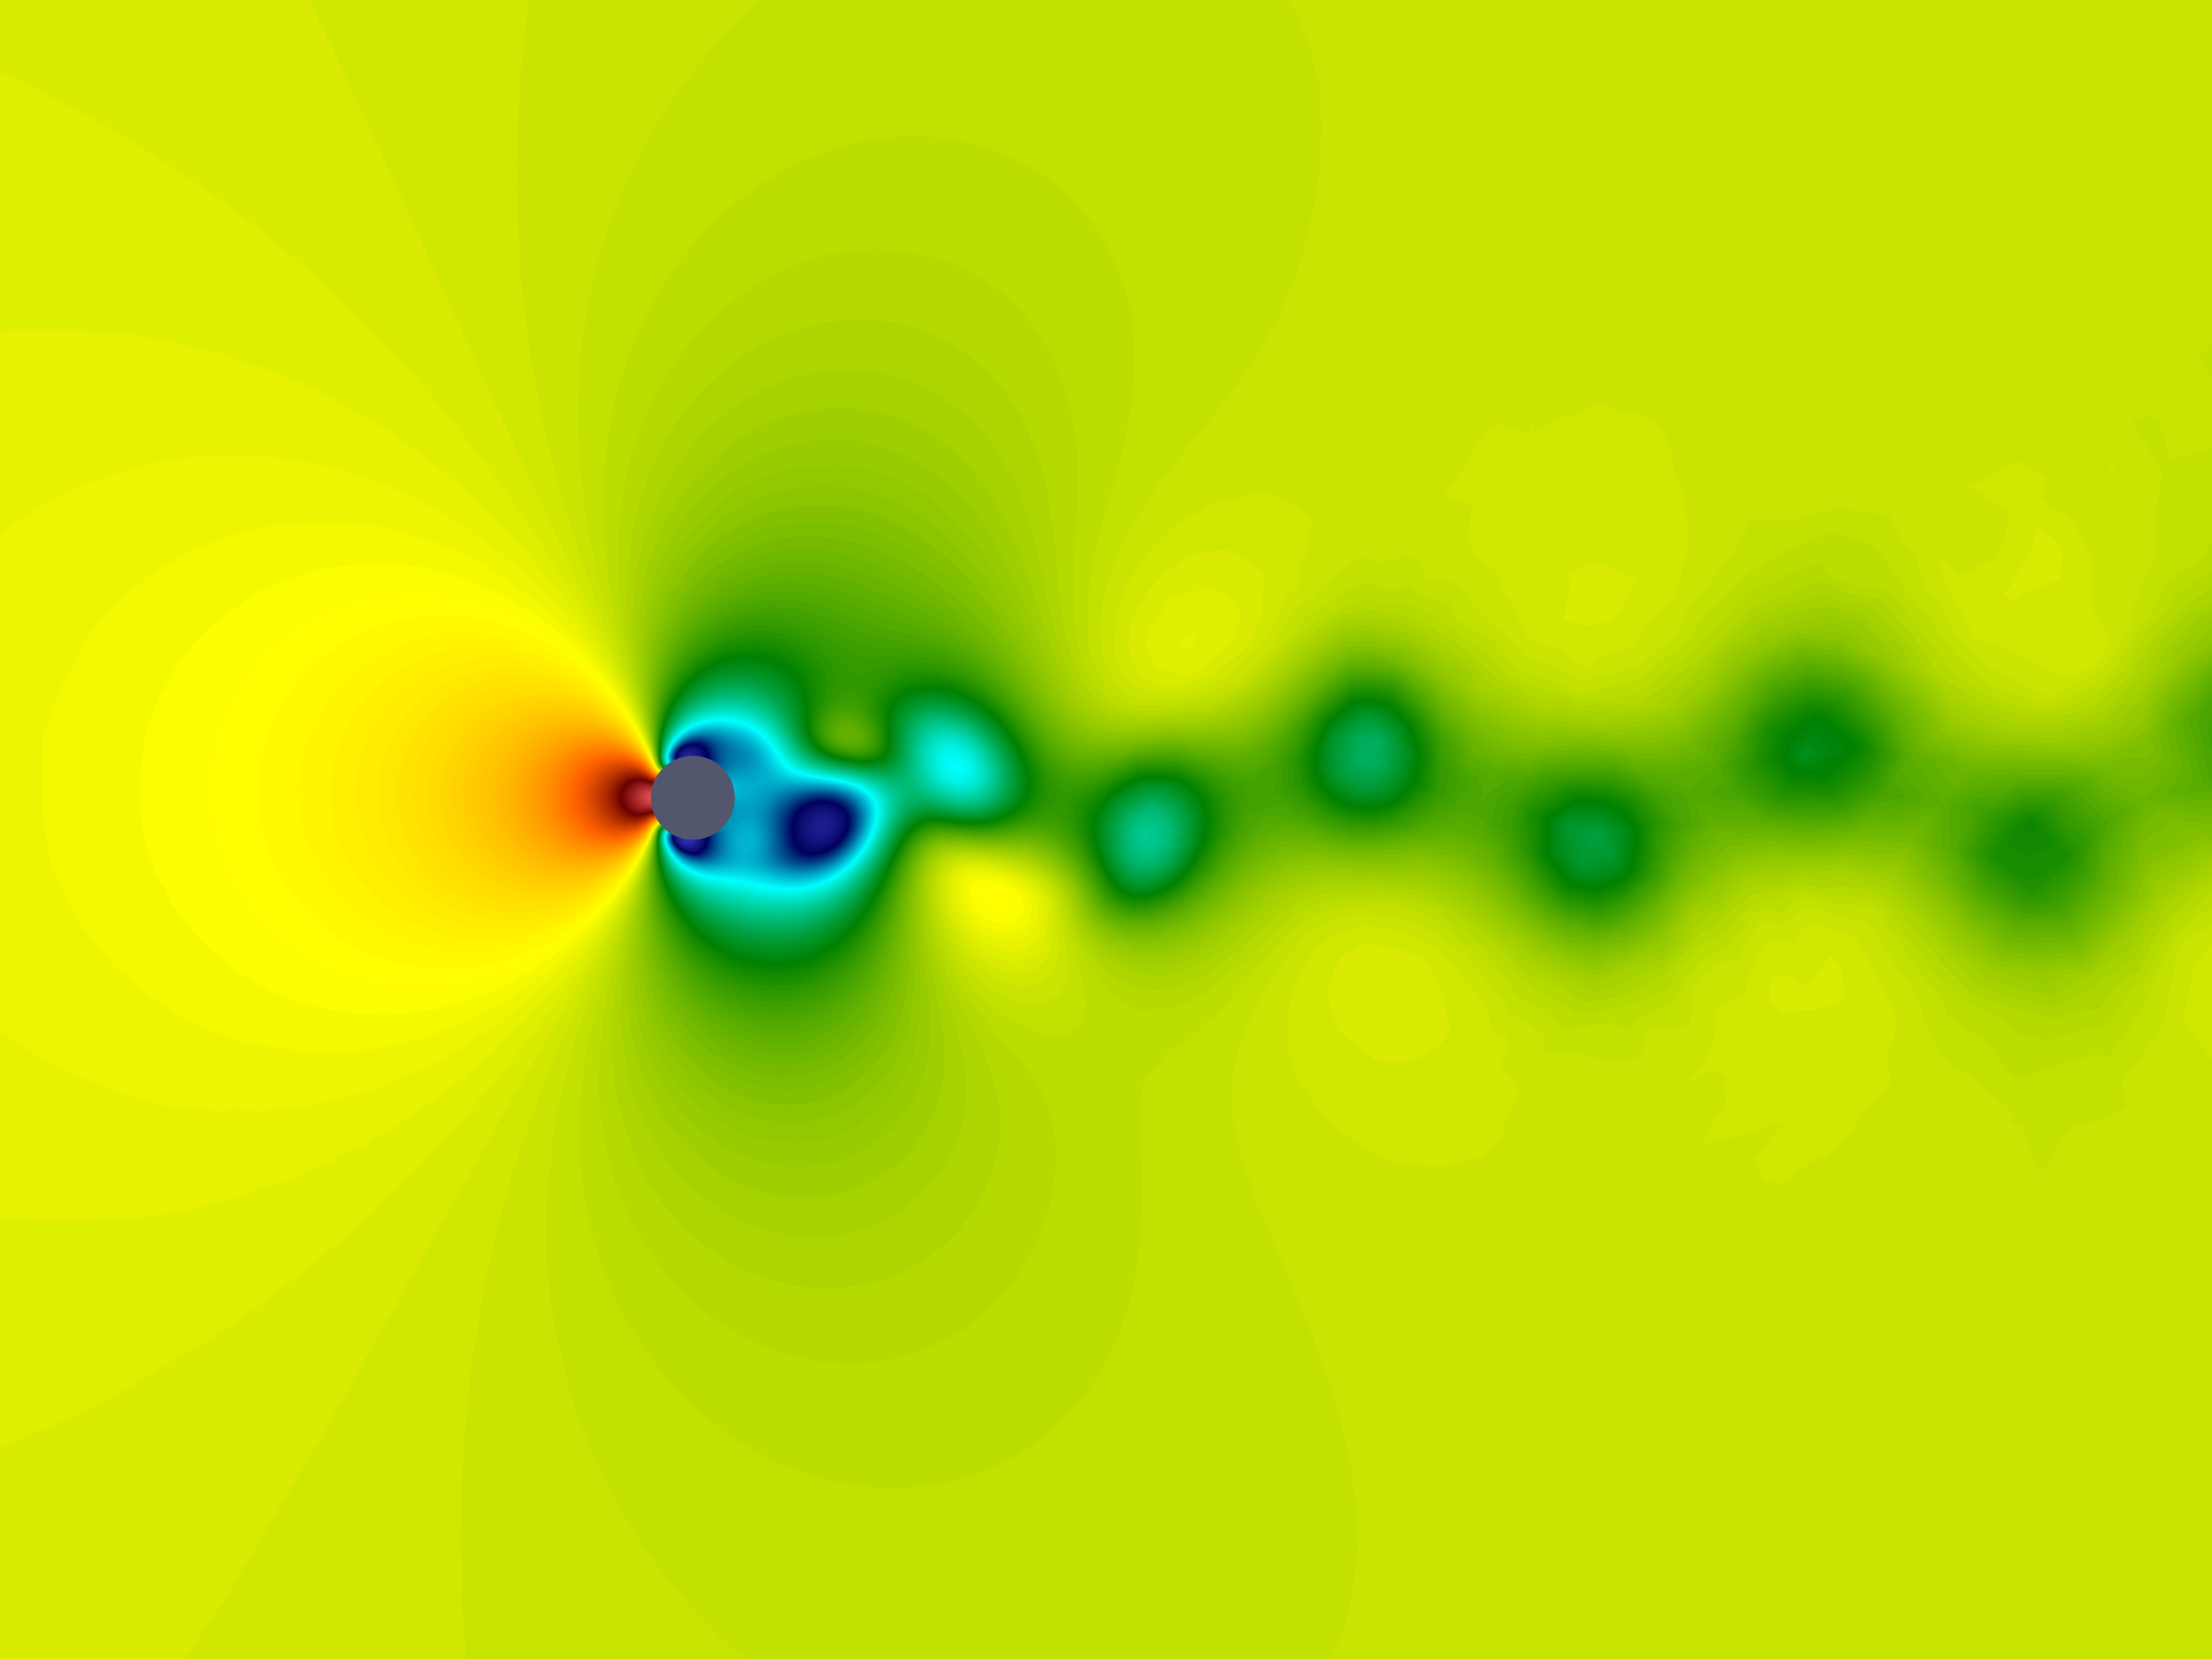
\includegraphics[scale=0.15,trim=5cm 5cm 5cm 6cm, clip=true]{Imagens/Cap2/cilindro_press2040.pdf}} \
	\subfloat[$T_n + T_n/2$]{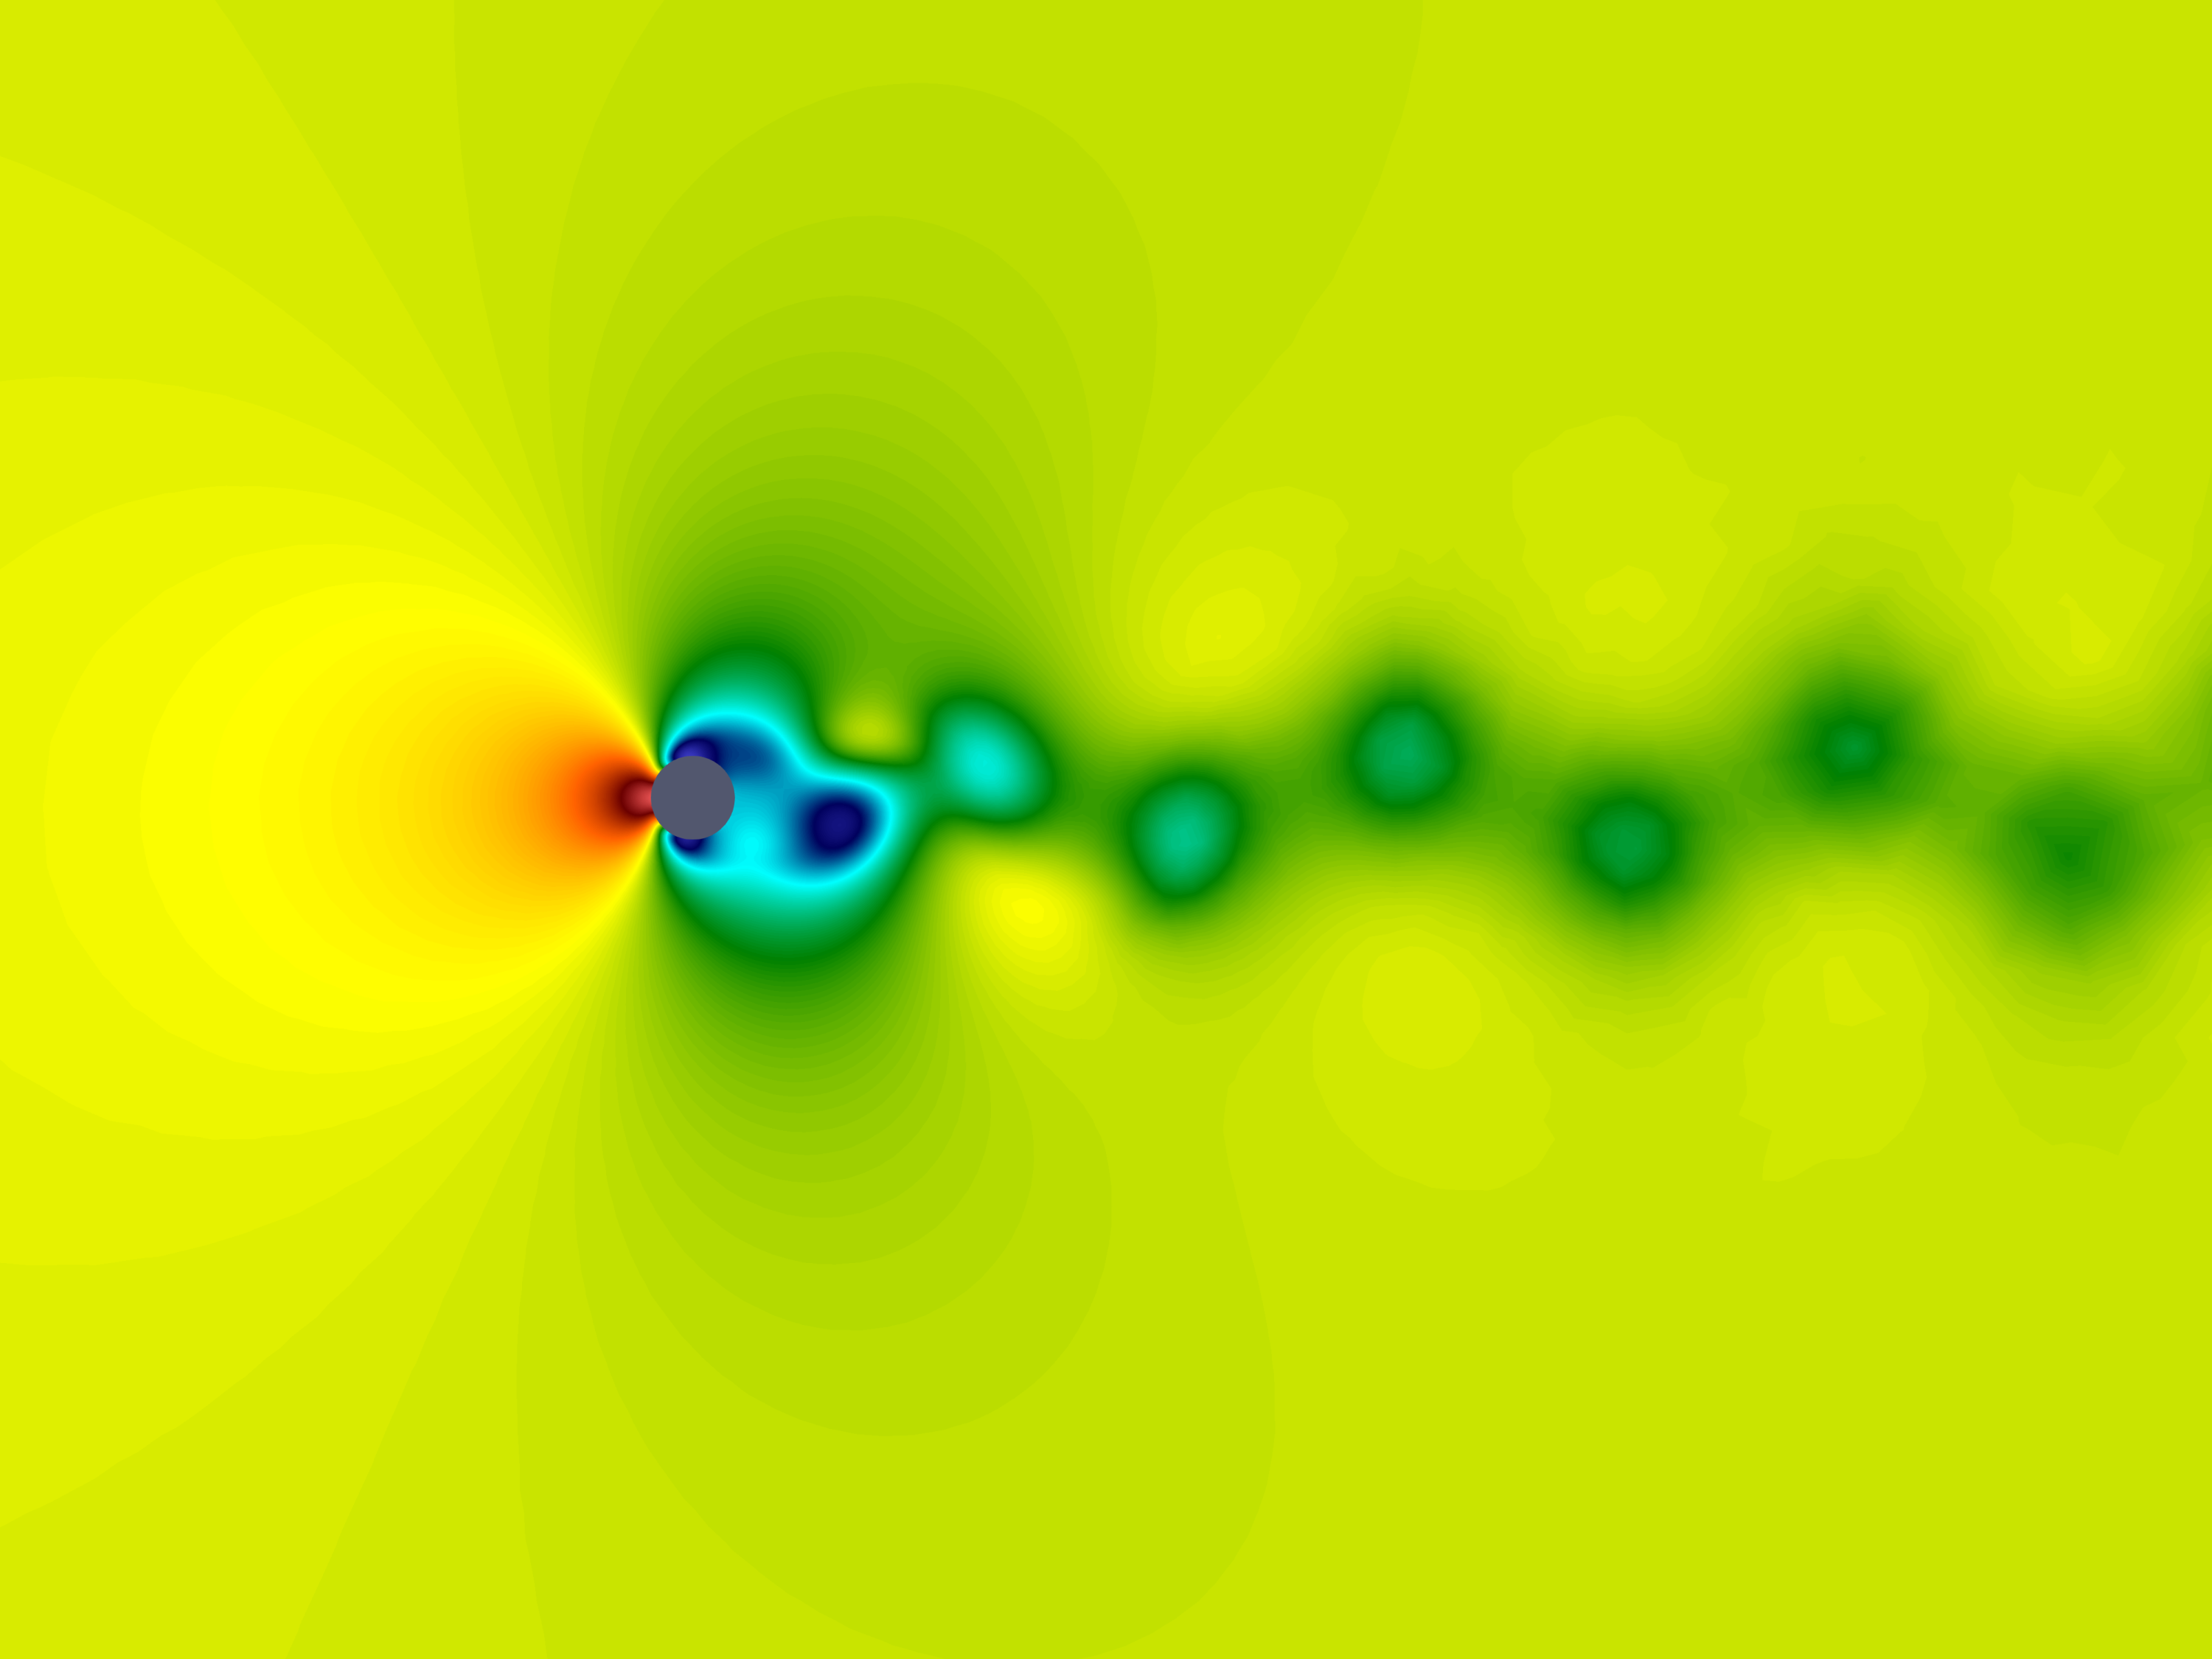
\includegraphics[scale=0.15,trim=5cm 5cm 5cm 6cm, clip=true]{Imagens/Cap2/cilindro_press2050.pdf}} \\
	\subfloat[$T_n + 2T_n/3$]{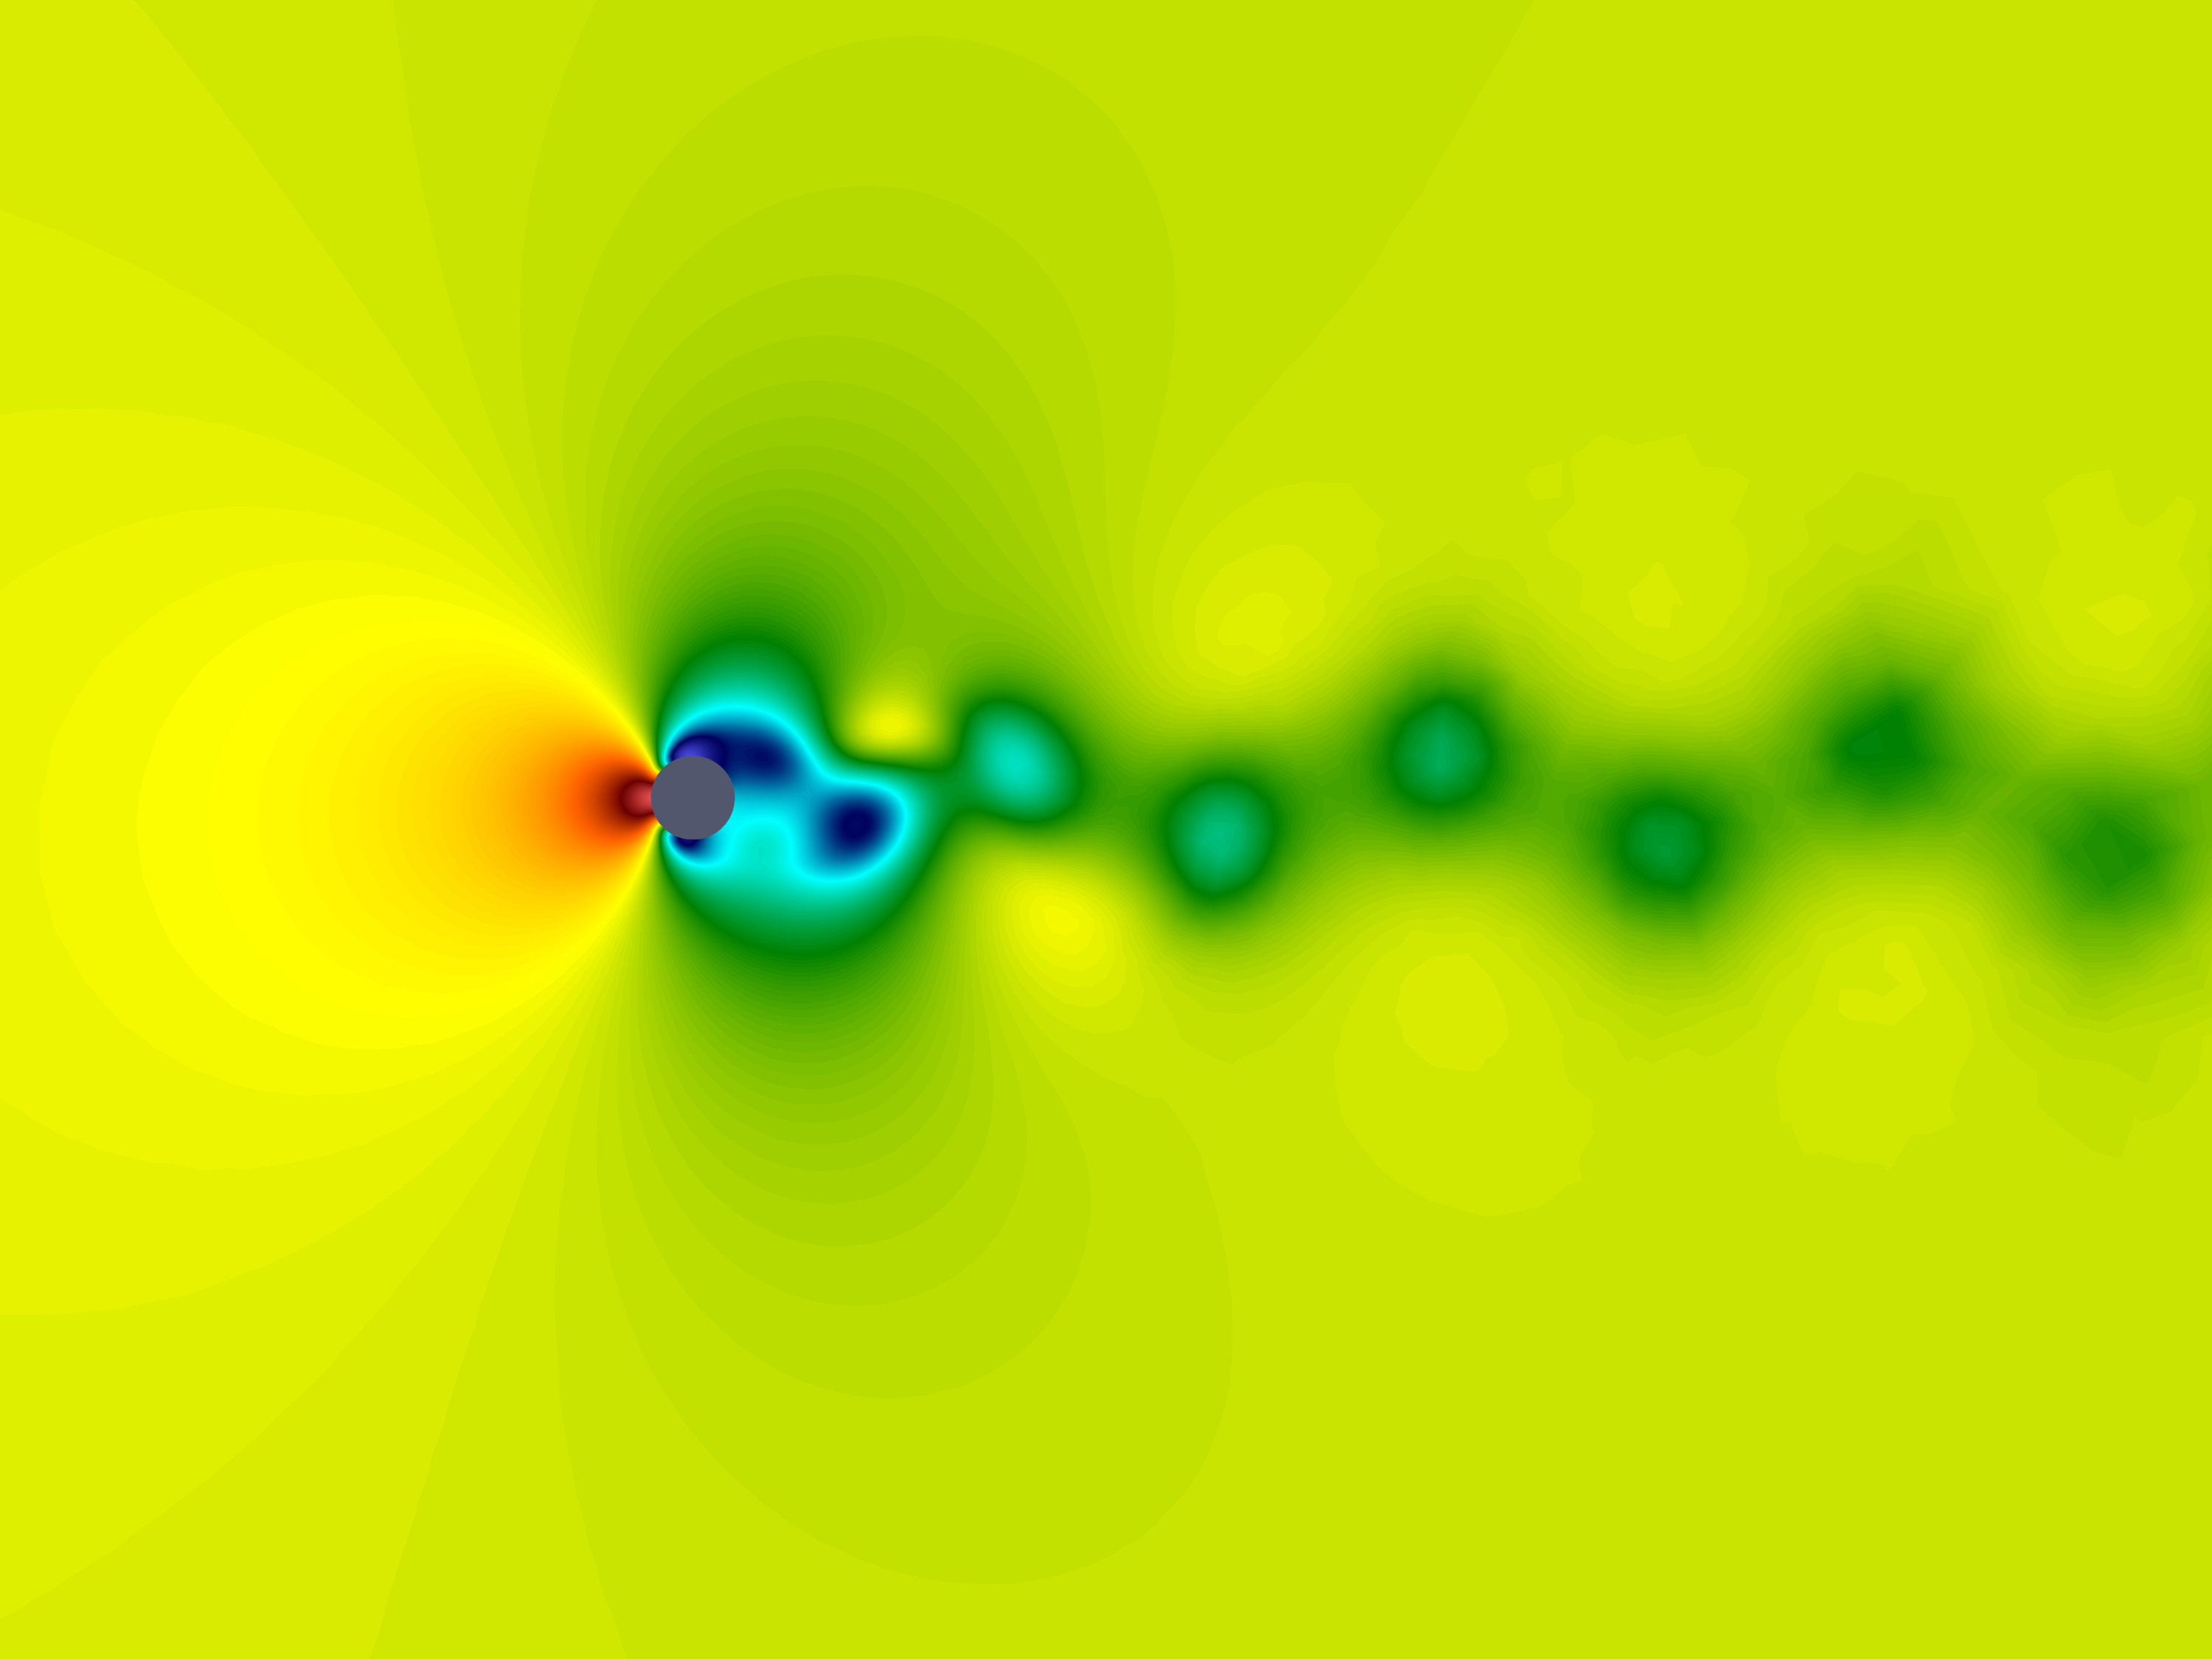
\includegraphics[scale=0.15,trim=5cm 5cm 5cm 6cm, clip=true]{Imagens/Cap2/cilindro_press2060.pdf}} \
	\subfloat[$T_n + 5T_n/6$]{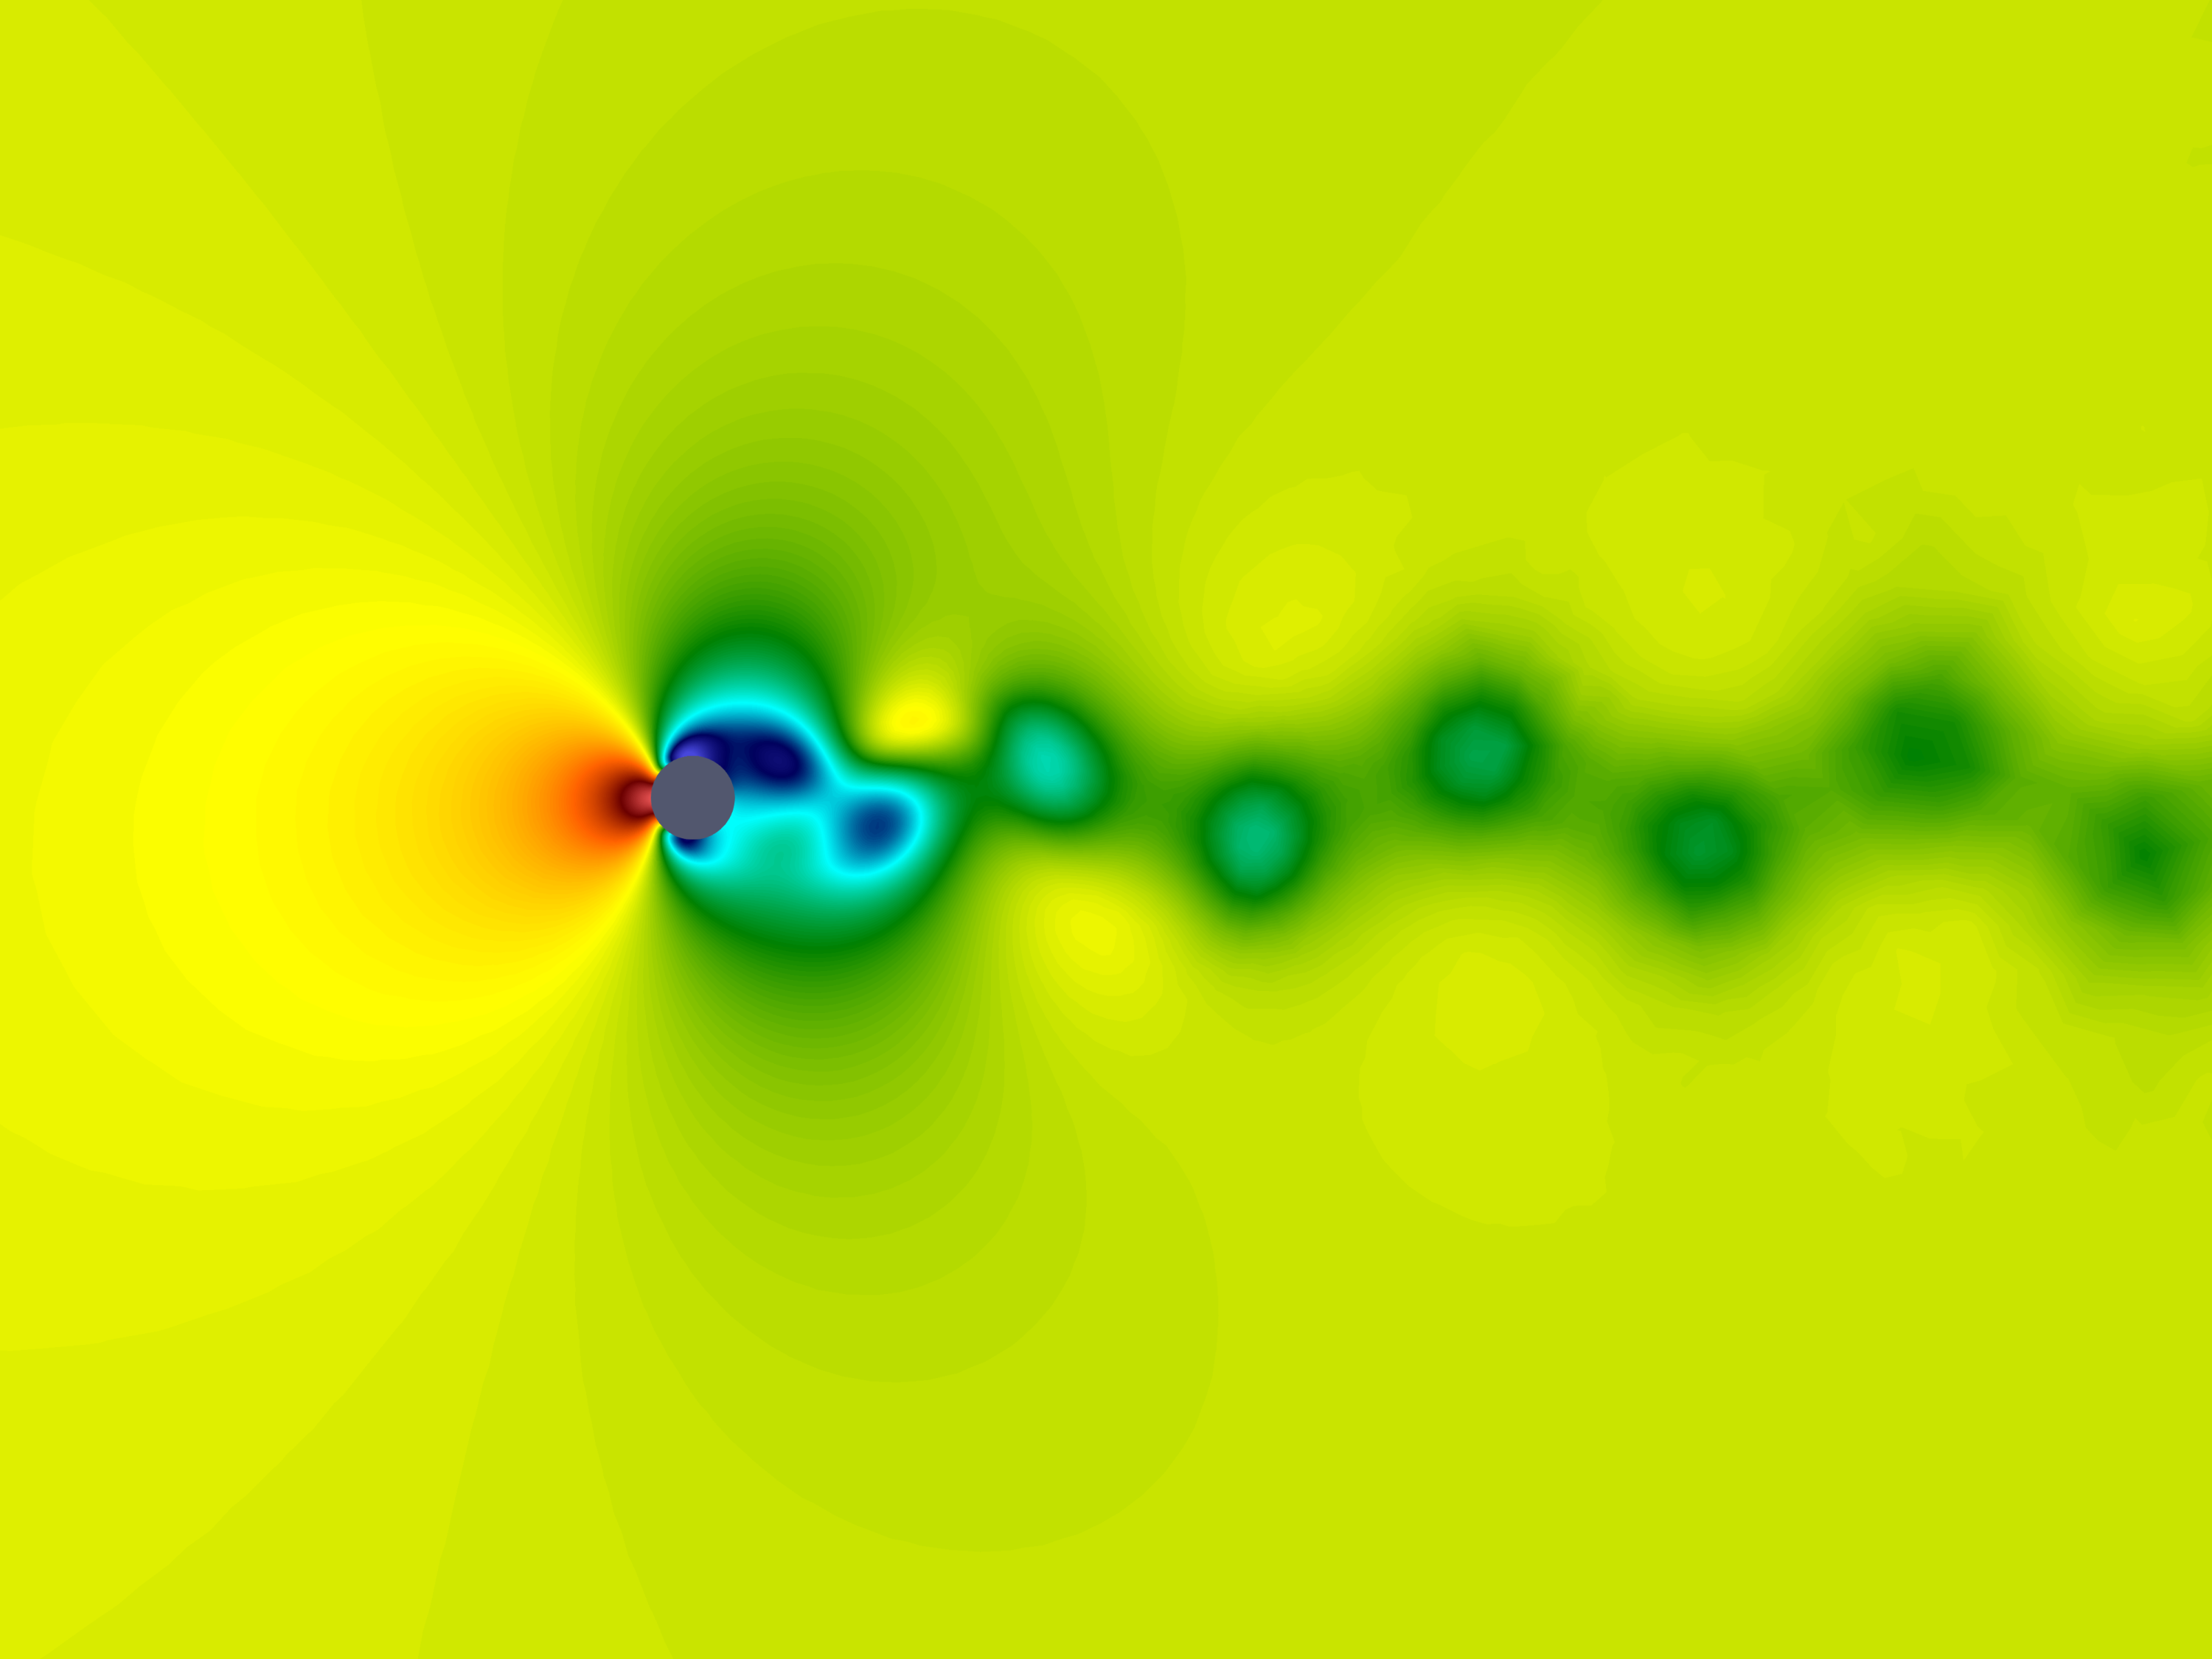
\includegraphics[scale=0.15,trim=5cm 5cm 5cm 6cm, clip=true]{Imagens/Cap2/cilindro_press2070.pdf}} \\
	{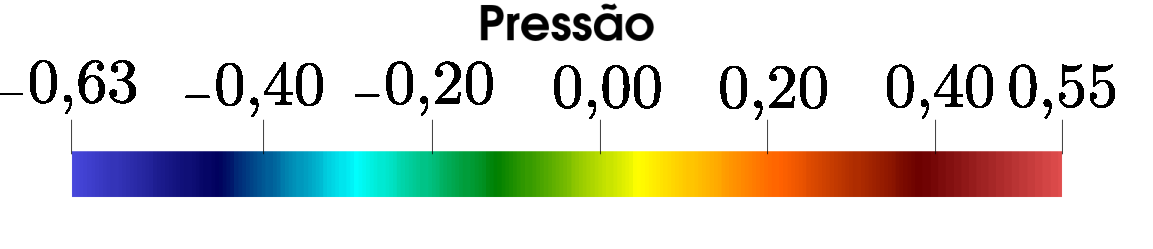
\includegraphics[trim=0cm 0cm 0cm 0cm,clip=true,scale=0.3]{Imagens/Cap2/cilindro_legendaPress.pdf}} \\
	\caption{Cilindro: Campos de pressão para $\Reynolds = 100$}
	\label{fig:cilindro_camposPressao}
\end{figure}


\subsection{Cavidade quadrada} \label{capitulo:Cap2:VerApl:CavQuad}

Para a verificação do código 3D utilizando elementos finitos o problema de uma cavidade quadrada com velocidade prescrita $u_{\infty}$ em sua parede superior foi estudado. A geometria do problema em questão e o conjunto de suas condições de contorno são apresentadas na Fig. \ref{fig:cavidade_geometria}. As paredes da cavidade são rígidas, com paredes laterais e do fundo com condição de aderência, e adicionalmente, condição de simetria na direção $y_3$. A cavidade possui na direção $y_3$ uma espessura de 0,03. A discretização espacial em elementos finitos utilizada é apresentada na Fig.  \ref{fig:cavidade_malha}, a qual consiste em 7252 elementos tetraédricos quadráticos e 14727 nós.

O problema é estudado para os números de Reynolds: 100, 400 e 1000. O número de Reynolds foi calculado de acordo com Eq. \eqref{eq:Reynolds}, com $L$ equivalente ao comprimento do lado da cavidade. O problema foi simulado para uma velocidade na parede superior de $u_{\infty} = 1,0$, $\density = 1,0$, $\timeStep = 0,05$, e $\specRadius = 0$, sendo a viscosidade do fluido variada de modo a alterar o número de Reynolds. A simulação foi mantida até que se atingiu o estado estacionário de escoamento. 

\begin{figure}[!htb]
	\centering
	\subfloat[Geometria e condições de contorno\label{fig:cavidade_geometria}]{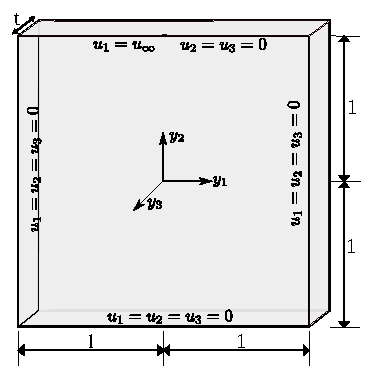
\includegraphics[scale=1.0,trim=0cm 0cm 0cm 0cm, clip=true]{Imagens/Cap2/cavidade_geometria.pdf}} \quad
	\subfloat[Discretização espacial.\label{fig:cavidade_malha}]{\includegraphics[trim=0 0 0 0,clip,scale=0.2]{Imagens/Cap2/cavidade_malha.png}}
	\caption{Cavidade quadrada: Geometria, condições de contorno e malha de elementos finitos}
\end{figure}

Os perfis de velocidade adimensionalizados ($\velocity/\velocinfty$) ao longo de duas linhas centrais nas direções $y_1$ e $y_2$ posicionadas no centro da espessura da direção $y_3$ da cavidade são apresentados na Fig. \ref{fig:cavidade_graficos} e comparados com a referência de \citeonline{GhiaGS:1982}.


\begin{figure}[!t]
	\centering
	\subfloat[\label{fig:cavidade_Re100}$Re$=100]{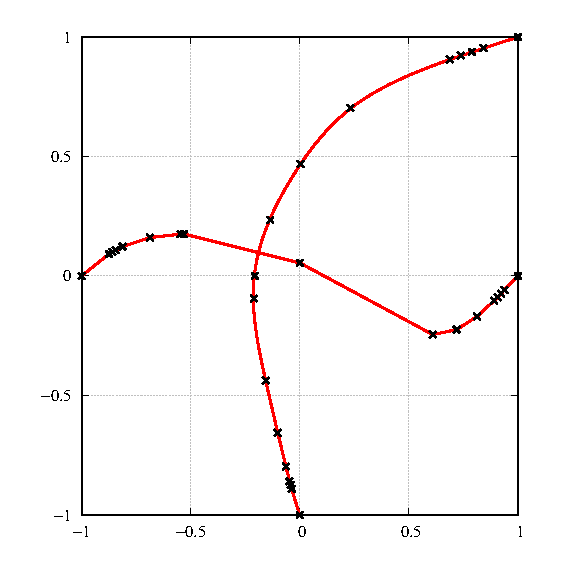
\includegraphics[scale=.8,trim=0.55cm 0cm 0.3cm 0.2cm, clip=true]{Imagens/Cap2/cavidade_Re100.eps}} \subfloat[\label{fig:cavidade_Re400}$Re$=400]{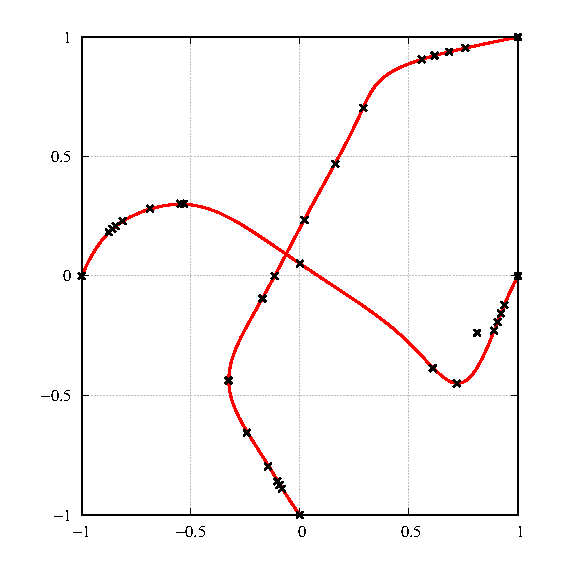
\includegraphics[scale=.8,trim=0.55cm 0cm 0.3cm 0.2cm, clip=true]{Imagens/Cap2/cavidade_Re400.eps}}\\ 
	\subfloat[\label{fig:cavidade_Re1000}$Re$=1000]{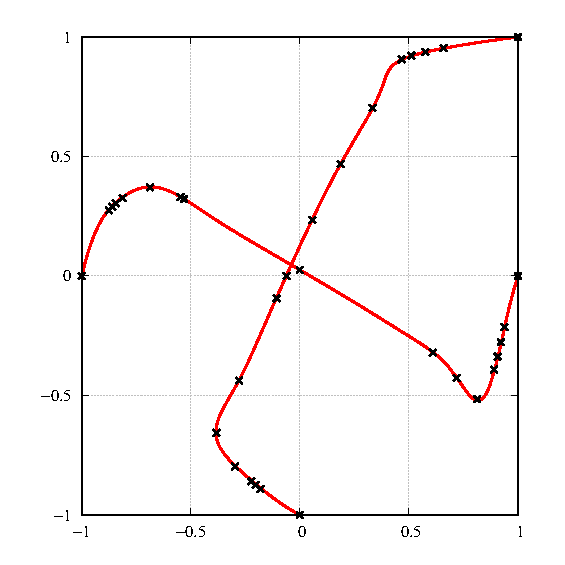
\includegraphics[scale=.8,trim=0.55cm 0cm 0.3cm 0.2cm, clip=true]{Imagens/Cap2/cavidade_Re1000.eps}} \\
	\subfloat{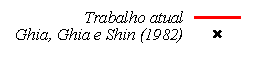
\includegraphics[scale=1.]{Imagens/Cap2/cavidade_legenda.pdf}} 
	\caption{Cavidade quadrada: Perfis de velocidade adimensionalizados nas direções $y_1$ e $y_2$  }
	\label{fig:cavidade_graficos}
\end{figure}

Os campos de velocidade e de pressão são apresentados nas figuras Fig \ref{fig:cavidade_vel} e \ref{fig:cavidade_press} respectivamente. Ressalta-se que para a solução do problema, por se tratar de um problema com todos os contornos com condição de Dirichlet impostos, a pressão torna-se indefinida. Por esse motivo, prescreveu-se uma pressão $\press = \press_{ref} =  0.0$ no canto superior direito da cavidade. 


\begin{figure}[!t]
	\centering
	\setlength{\lineskip}{-10pt}
	\subfloat[\label{fig:cavidade_vel_Re100}$Re$=100]{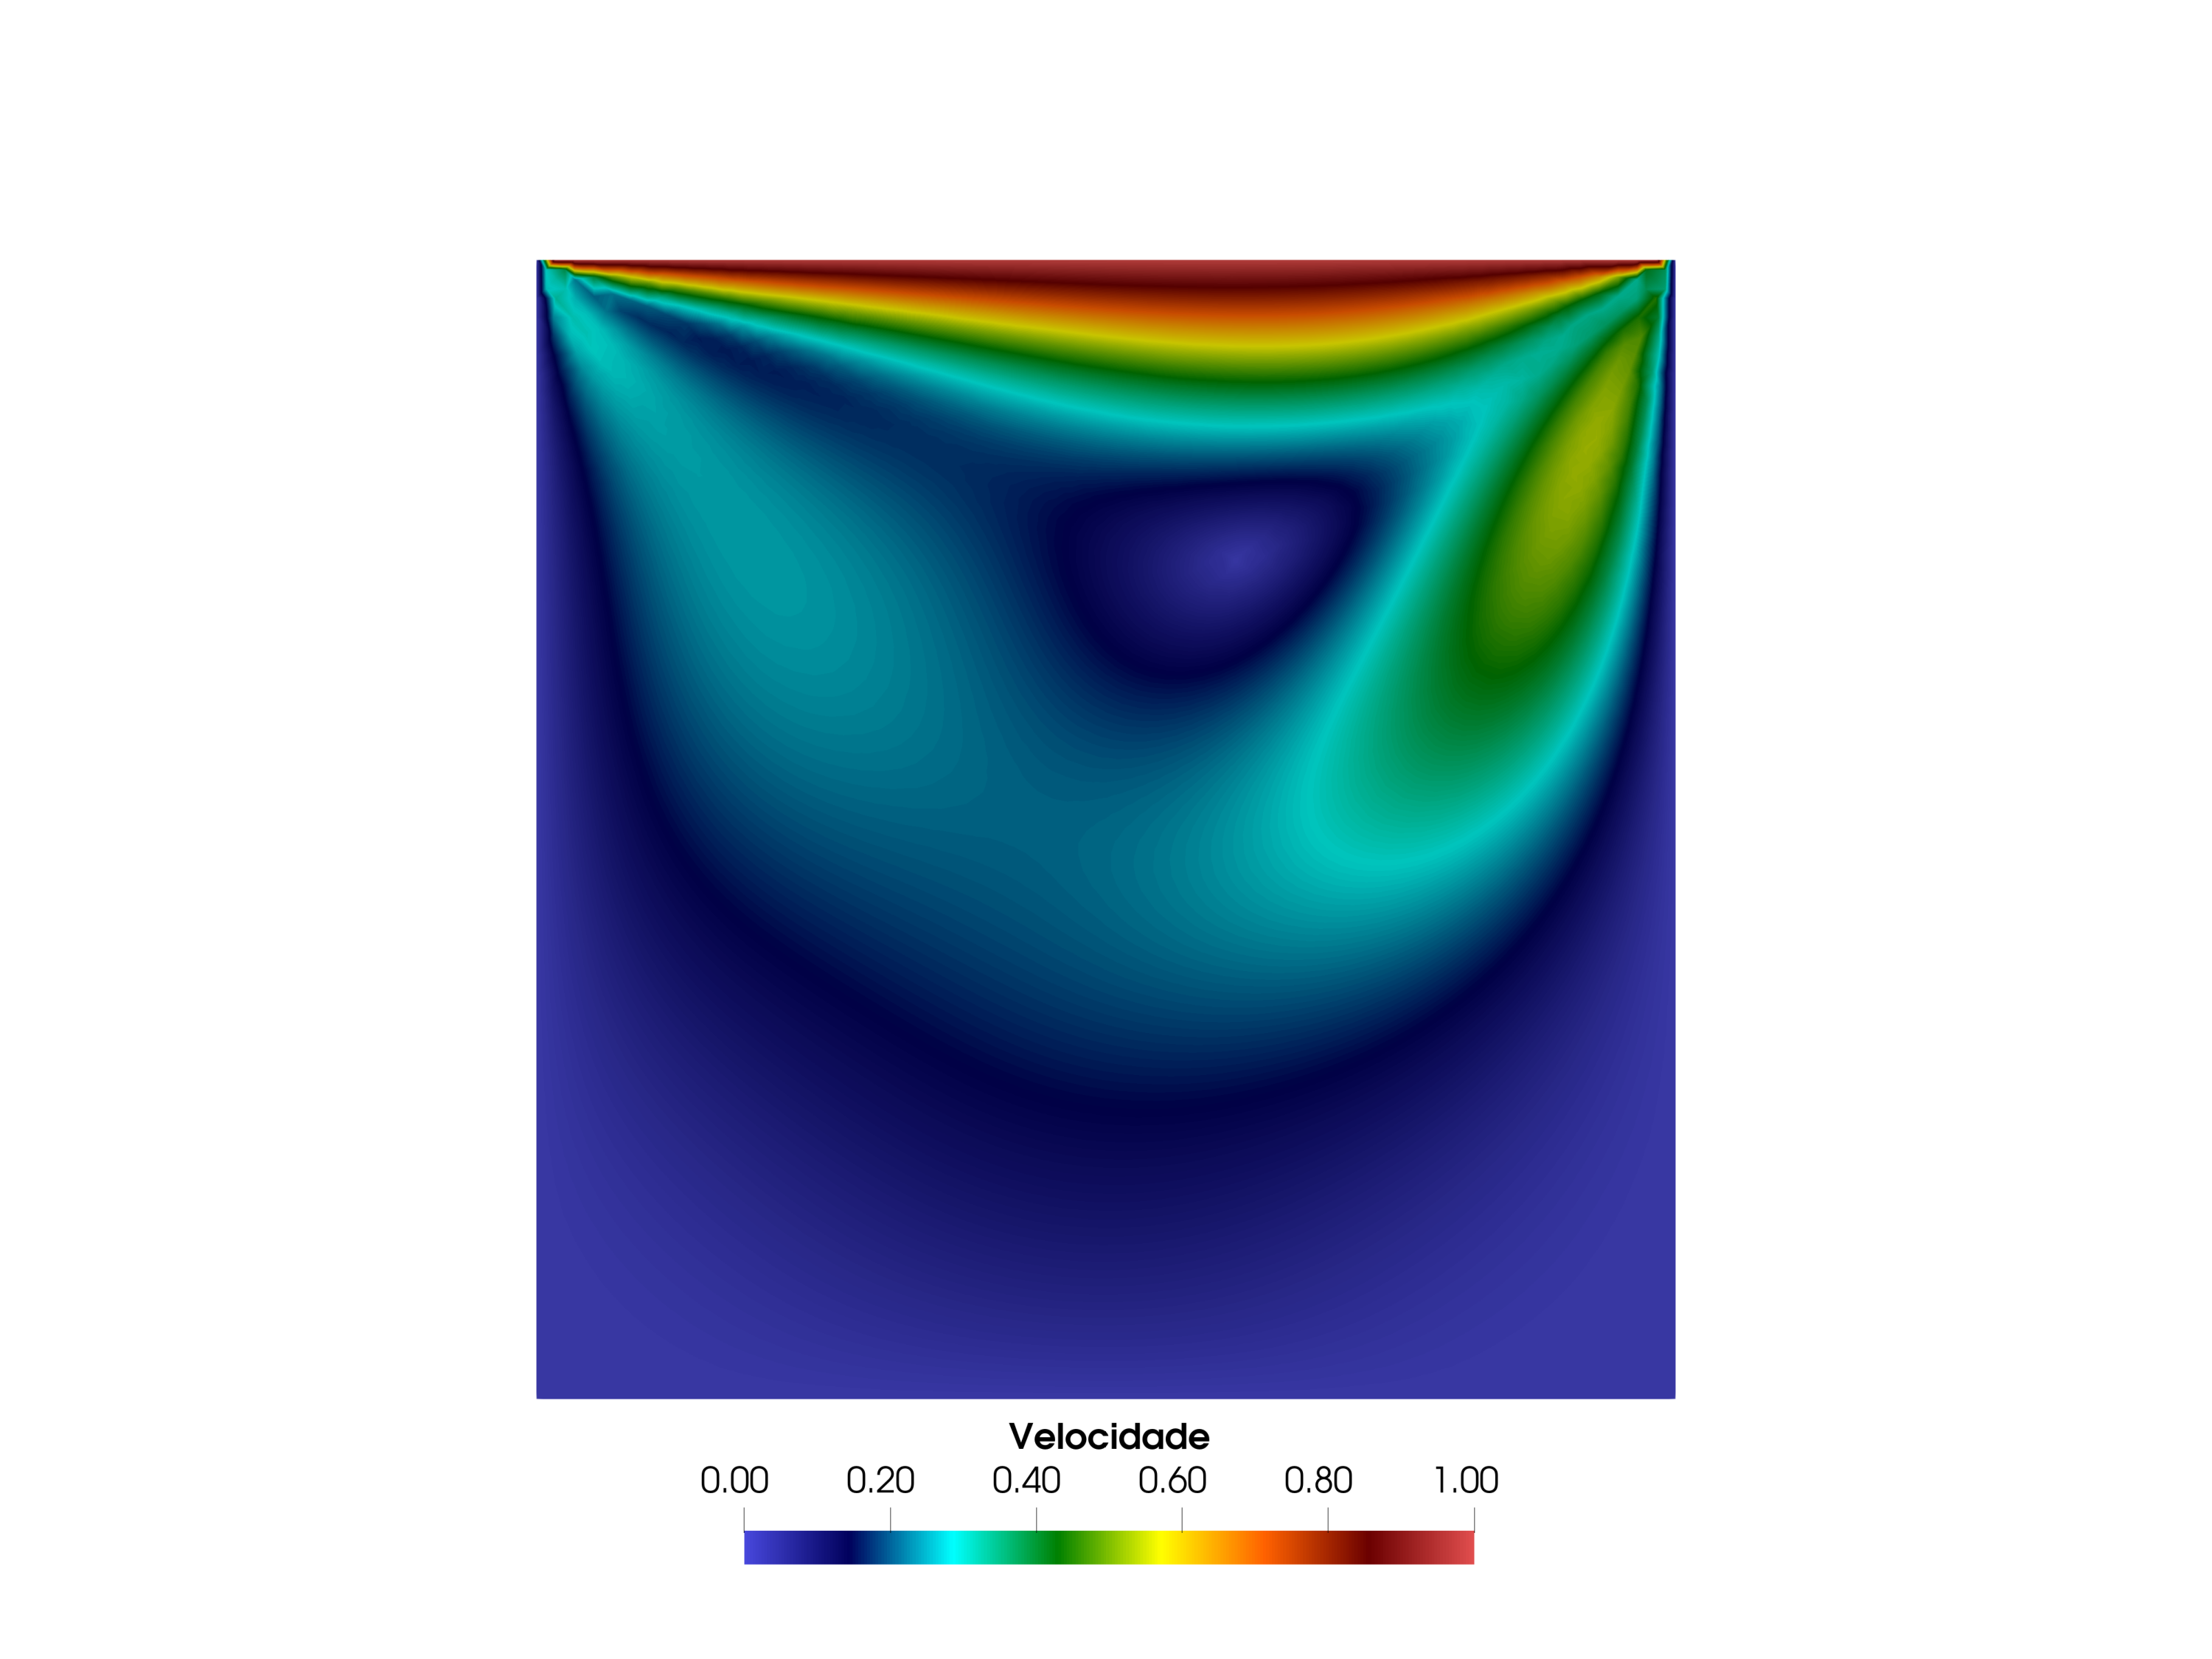
\includegraphics[scale=0.25,trim=12cm 5.5cm 12cm 5cm, clip=true]{Imagens/Cap2/cavidade_velRe100.pdf}} 
	\subfloat[\label{fig:cavidade_vel_Re400}$Re$=400]{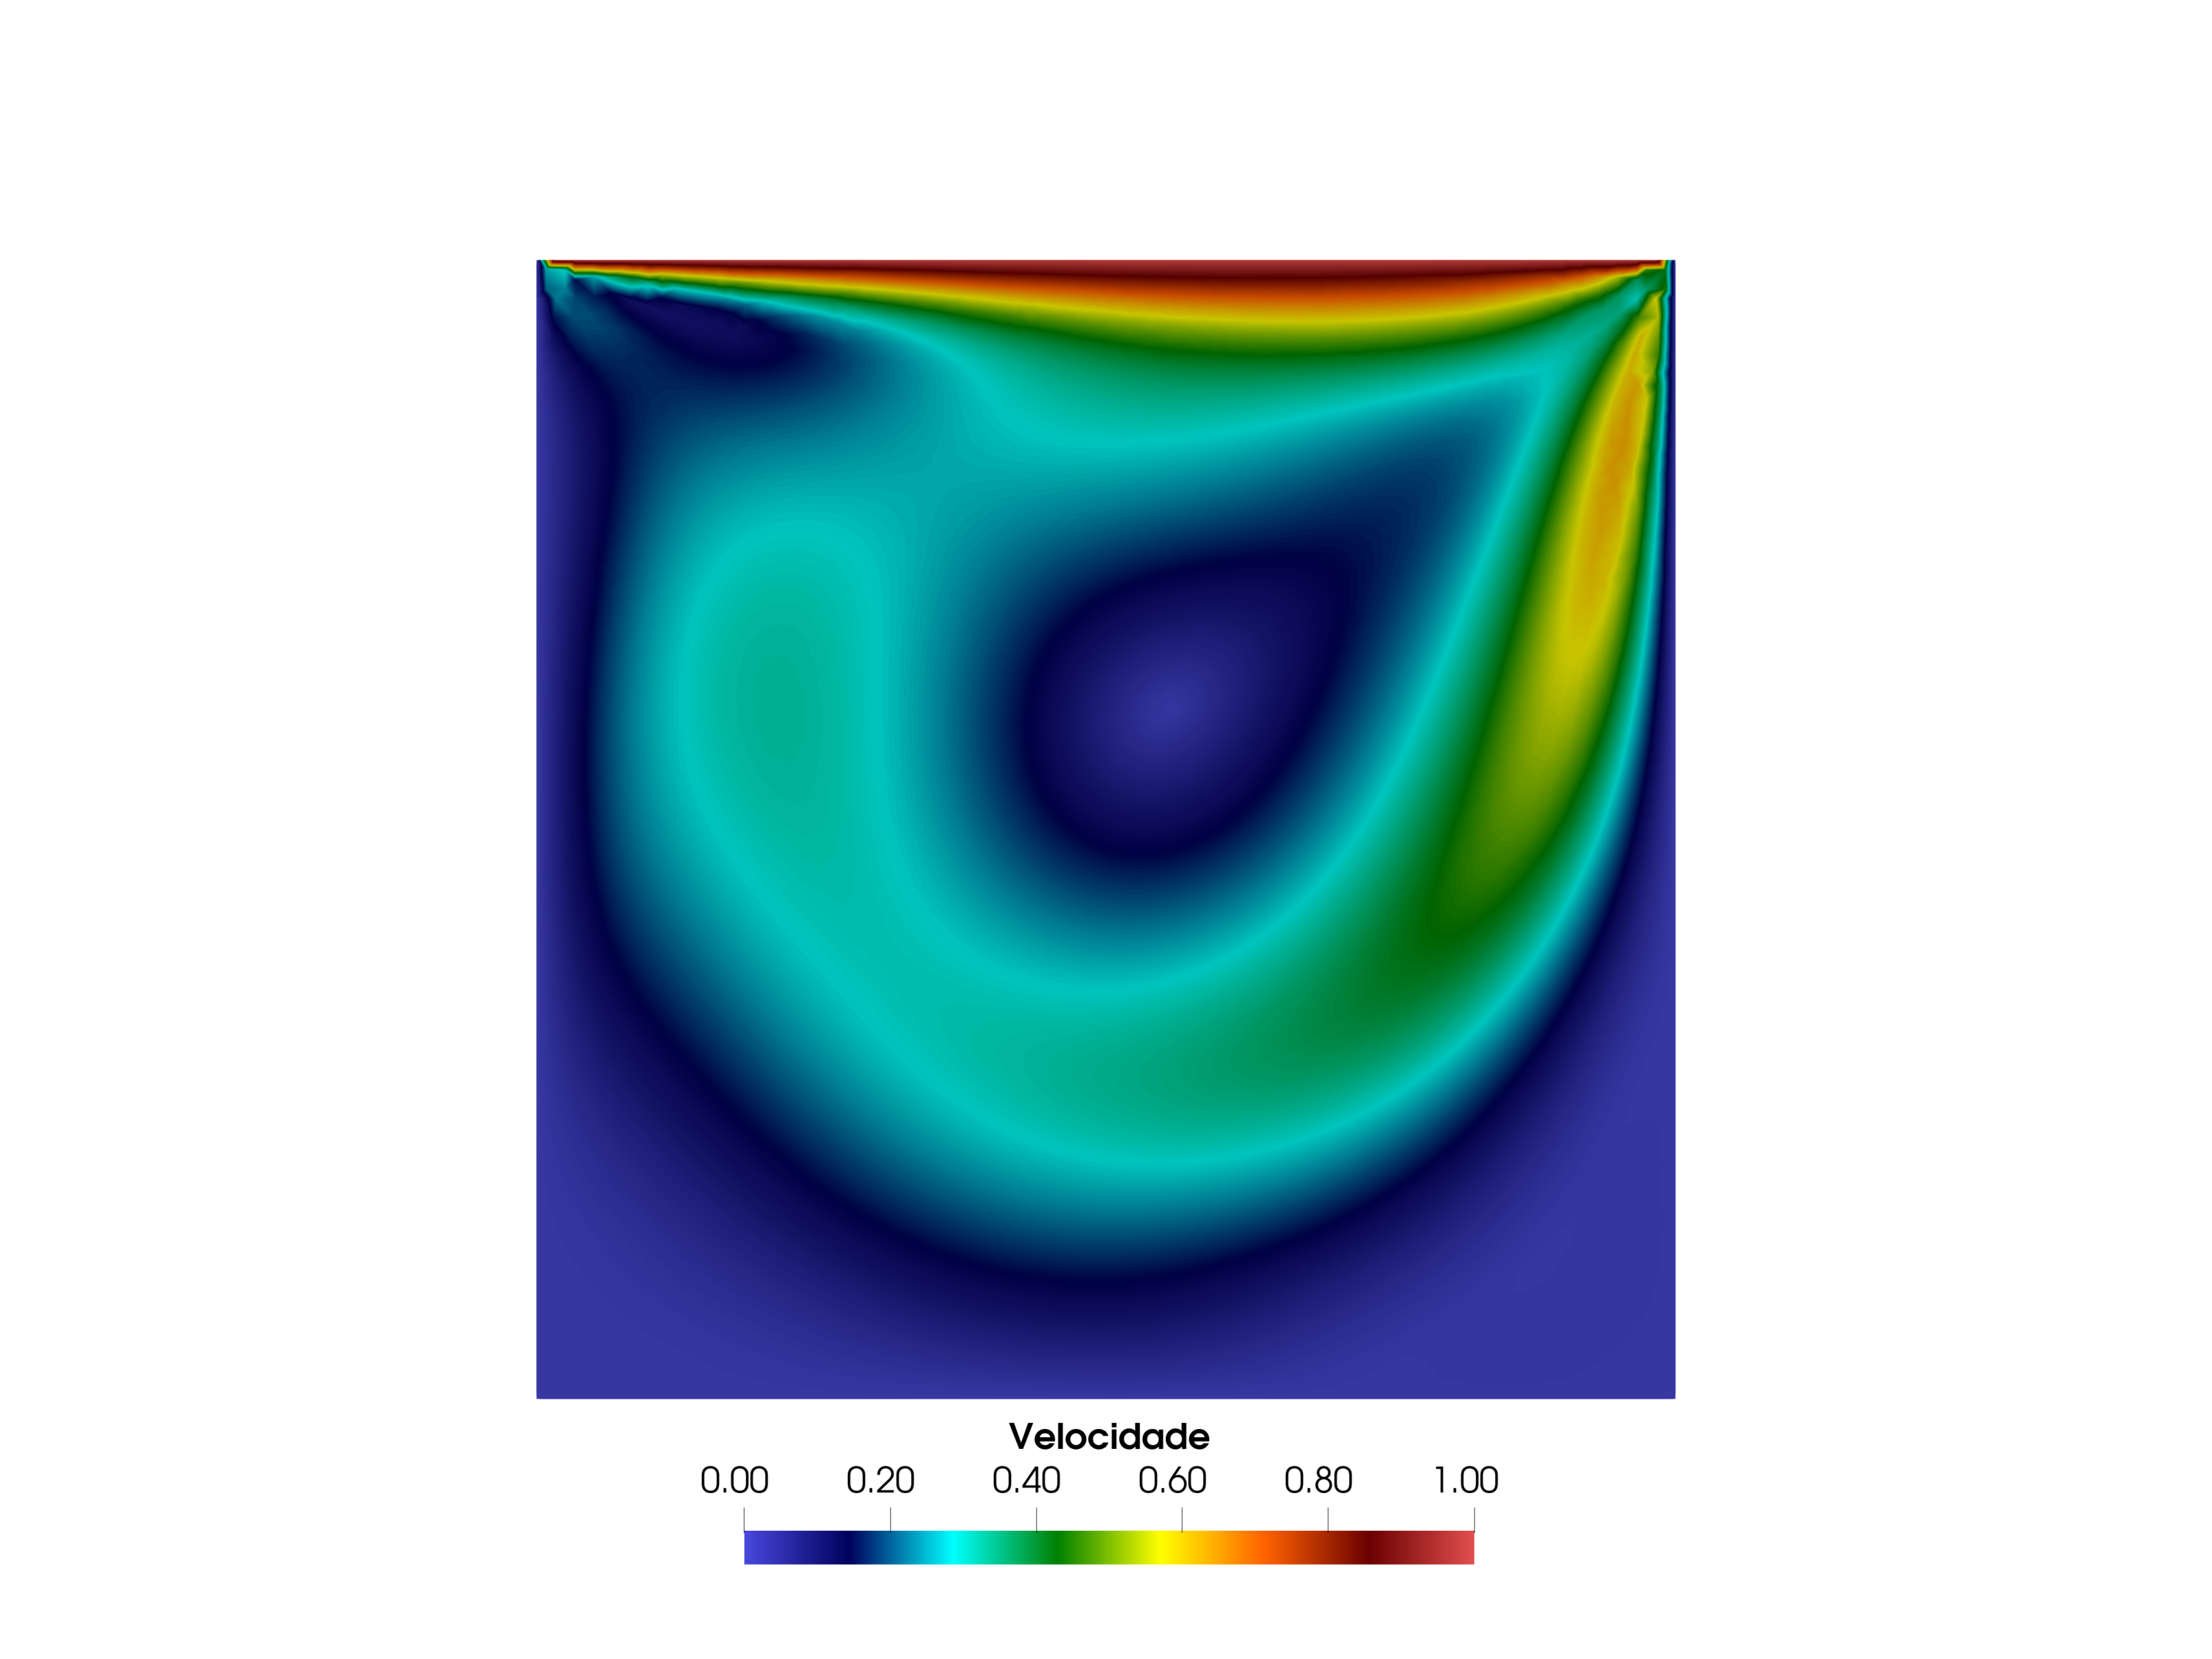
\includegraphics[scale=0.25,trim=12cm 5.5cm 12cm 5cm, clip=true]{Imagens/Cap2/cavidade_velRe400.pdf}}\\ 
	\subfloat[\label{fig:cavidade_vel_Re1000}$Re$=1000]{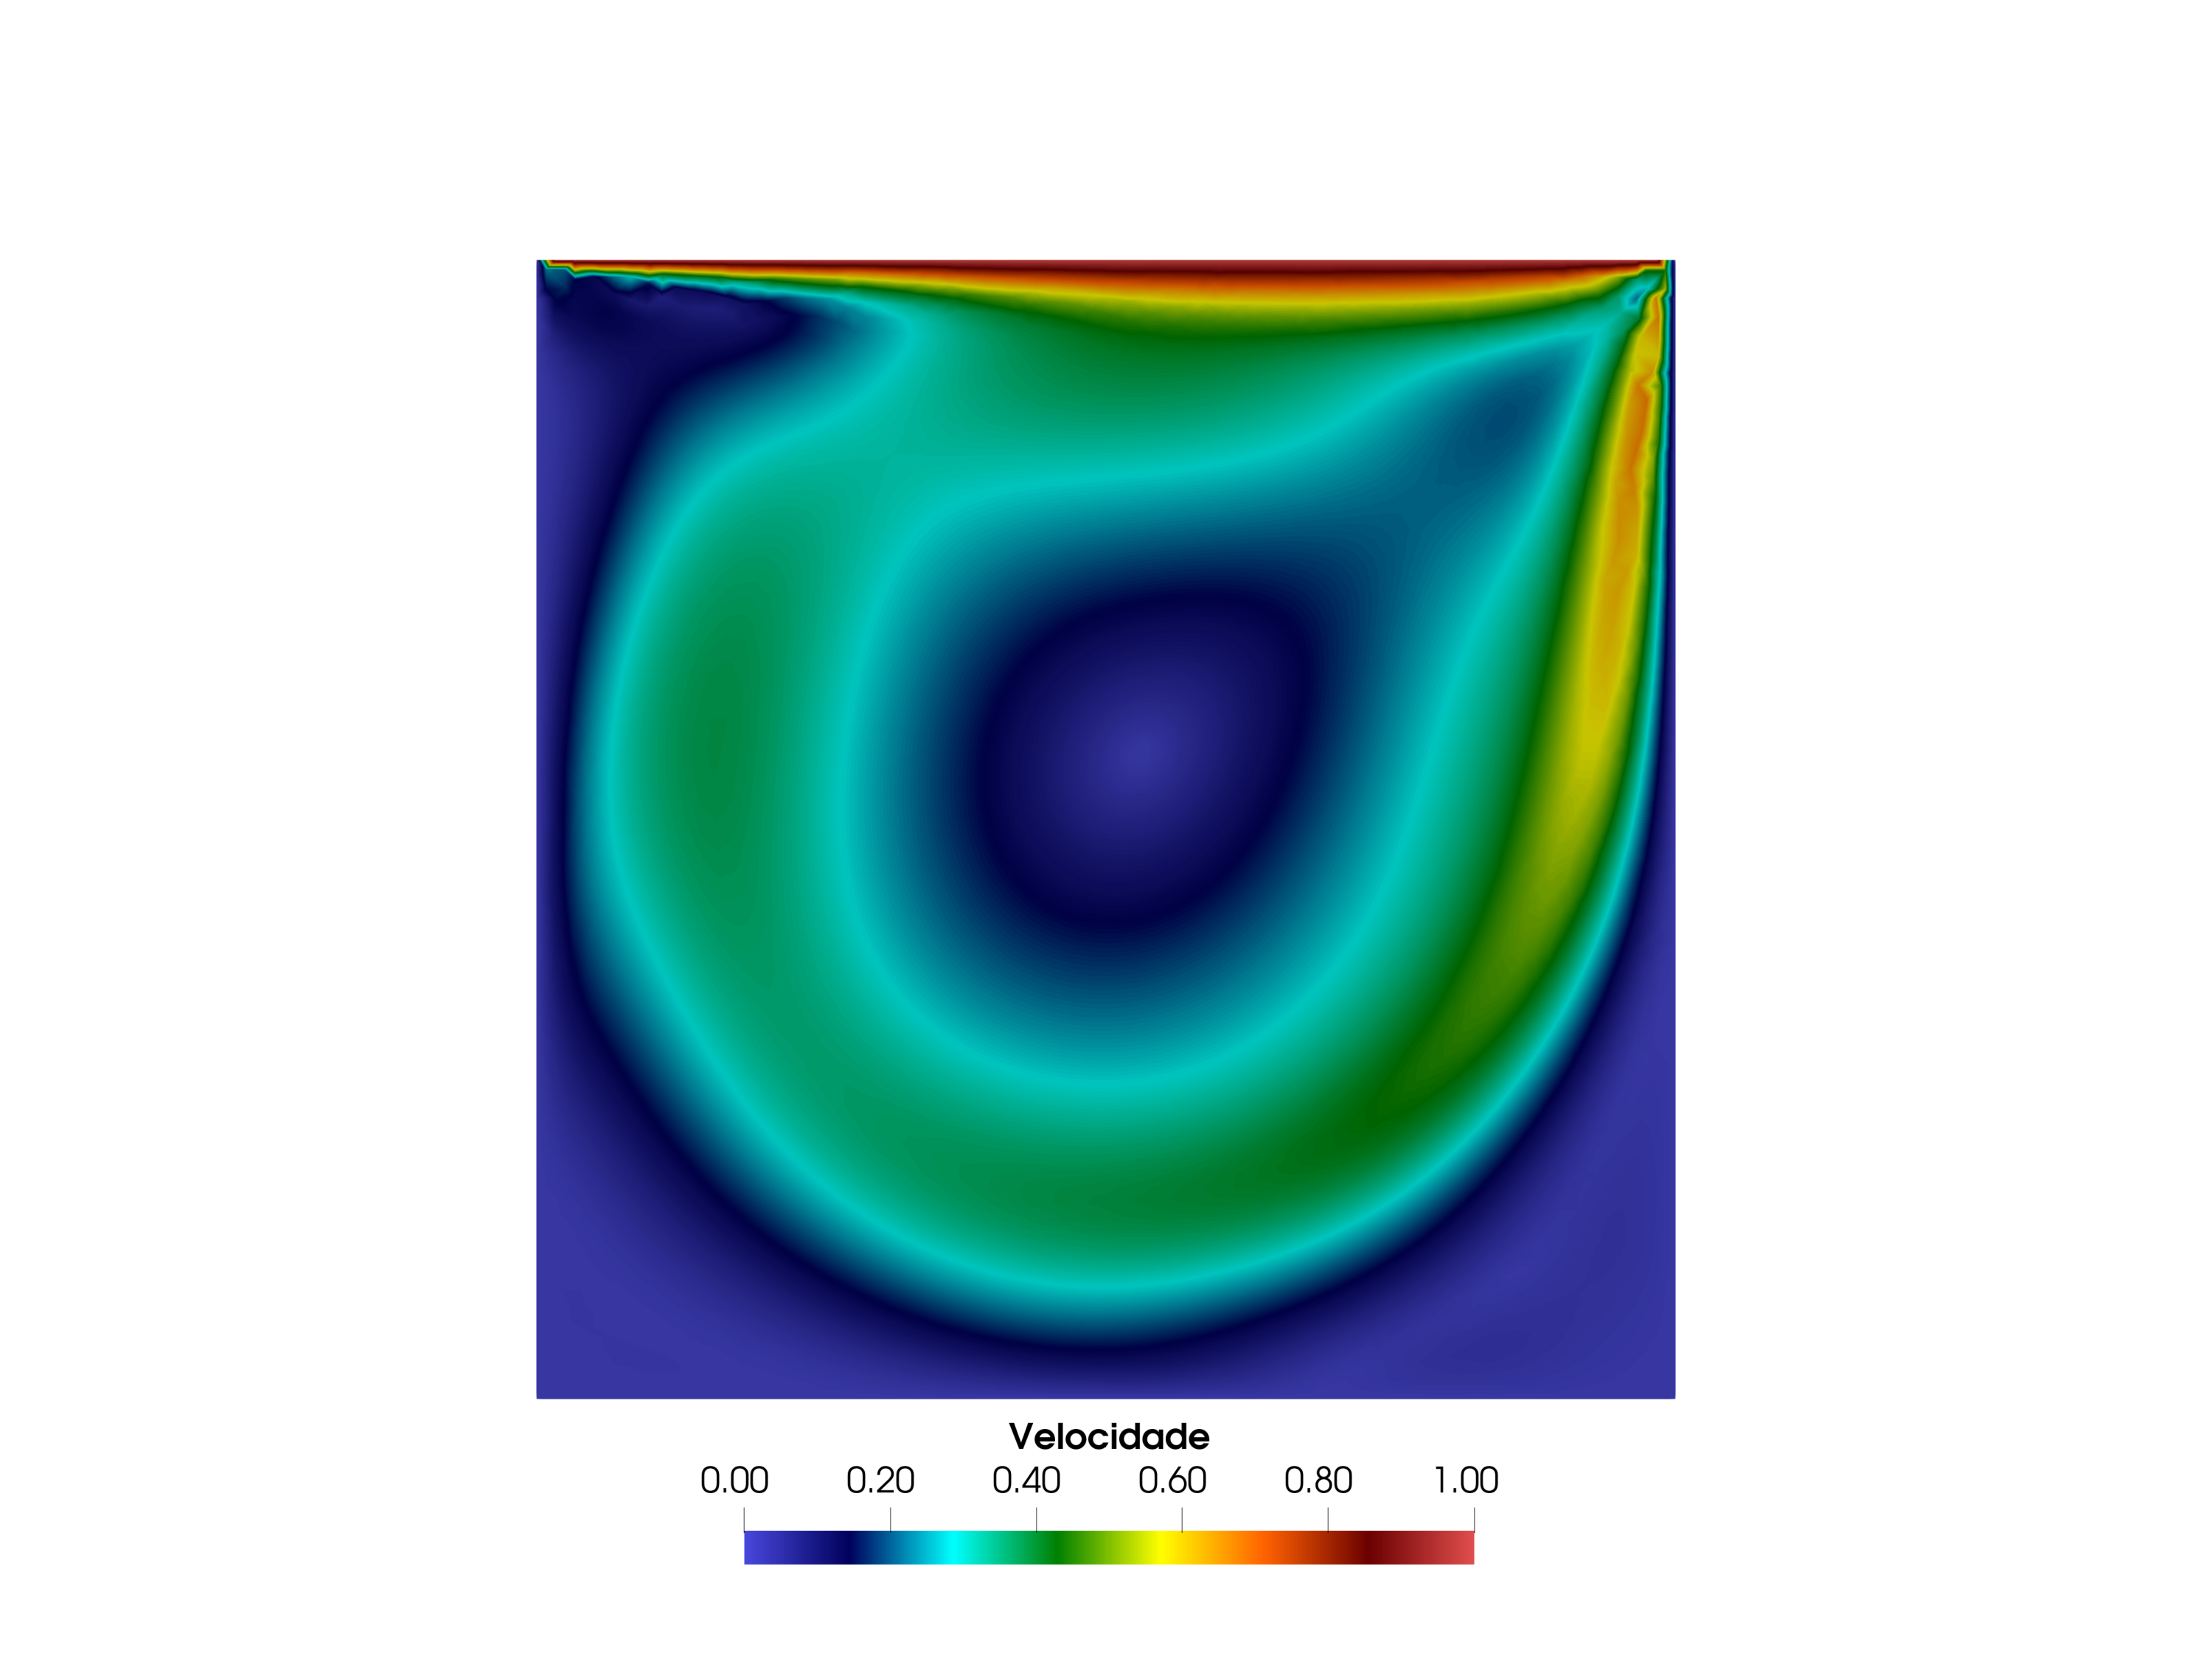
\includegraphics[scale=0.25,trim=12cm 5.5cm 12cm 5cm, clip=true]{Imagens/Cap2/cavidade_velRe1000.pdf}}\\[3.0ex]
	% Barra de cores (legenda) separada
	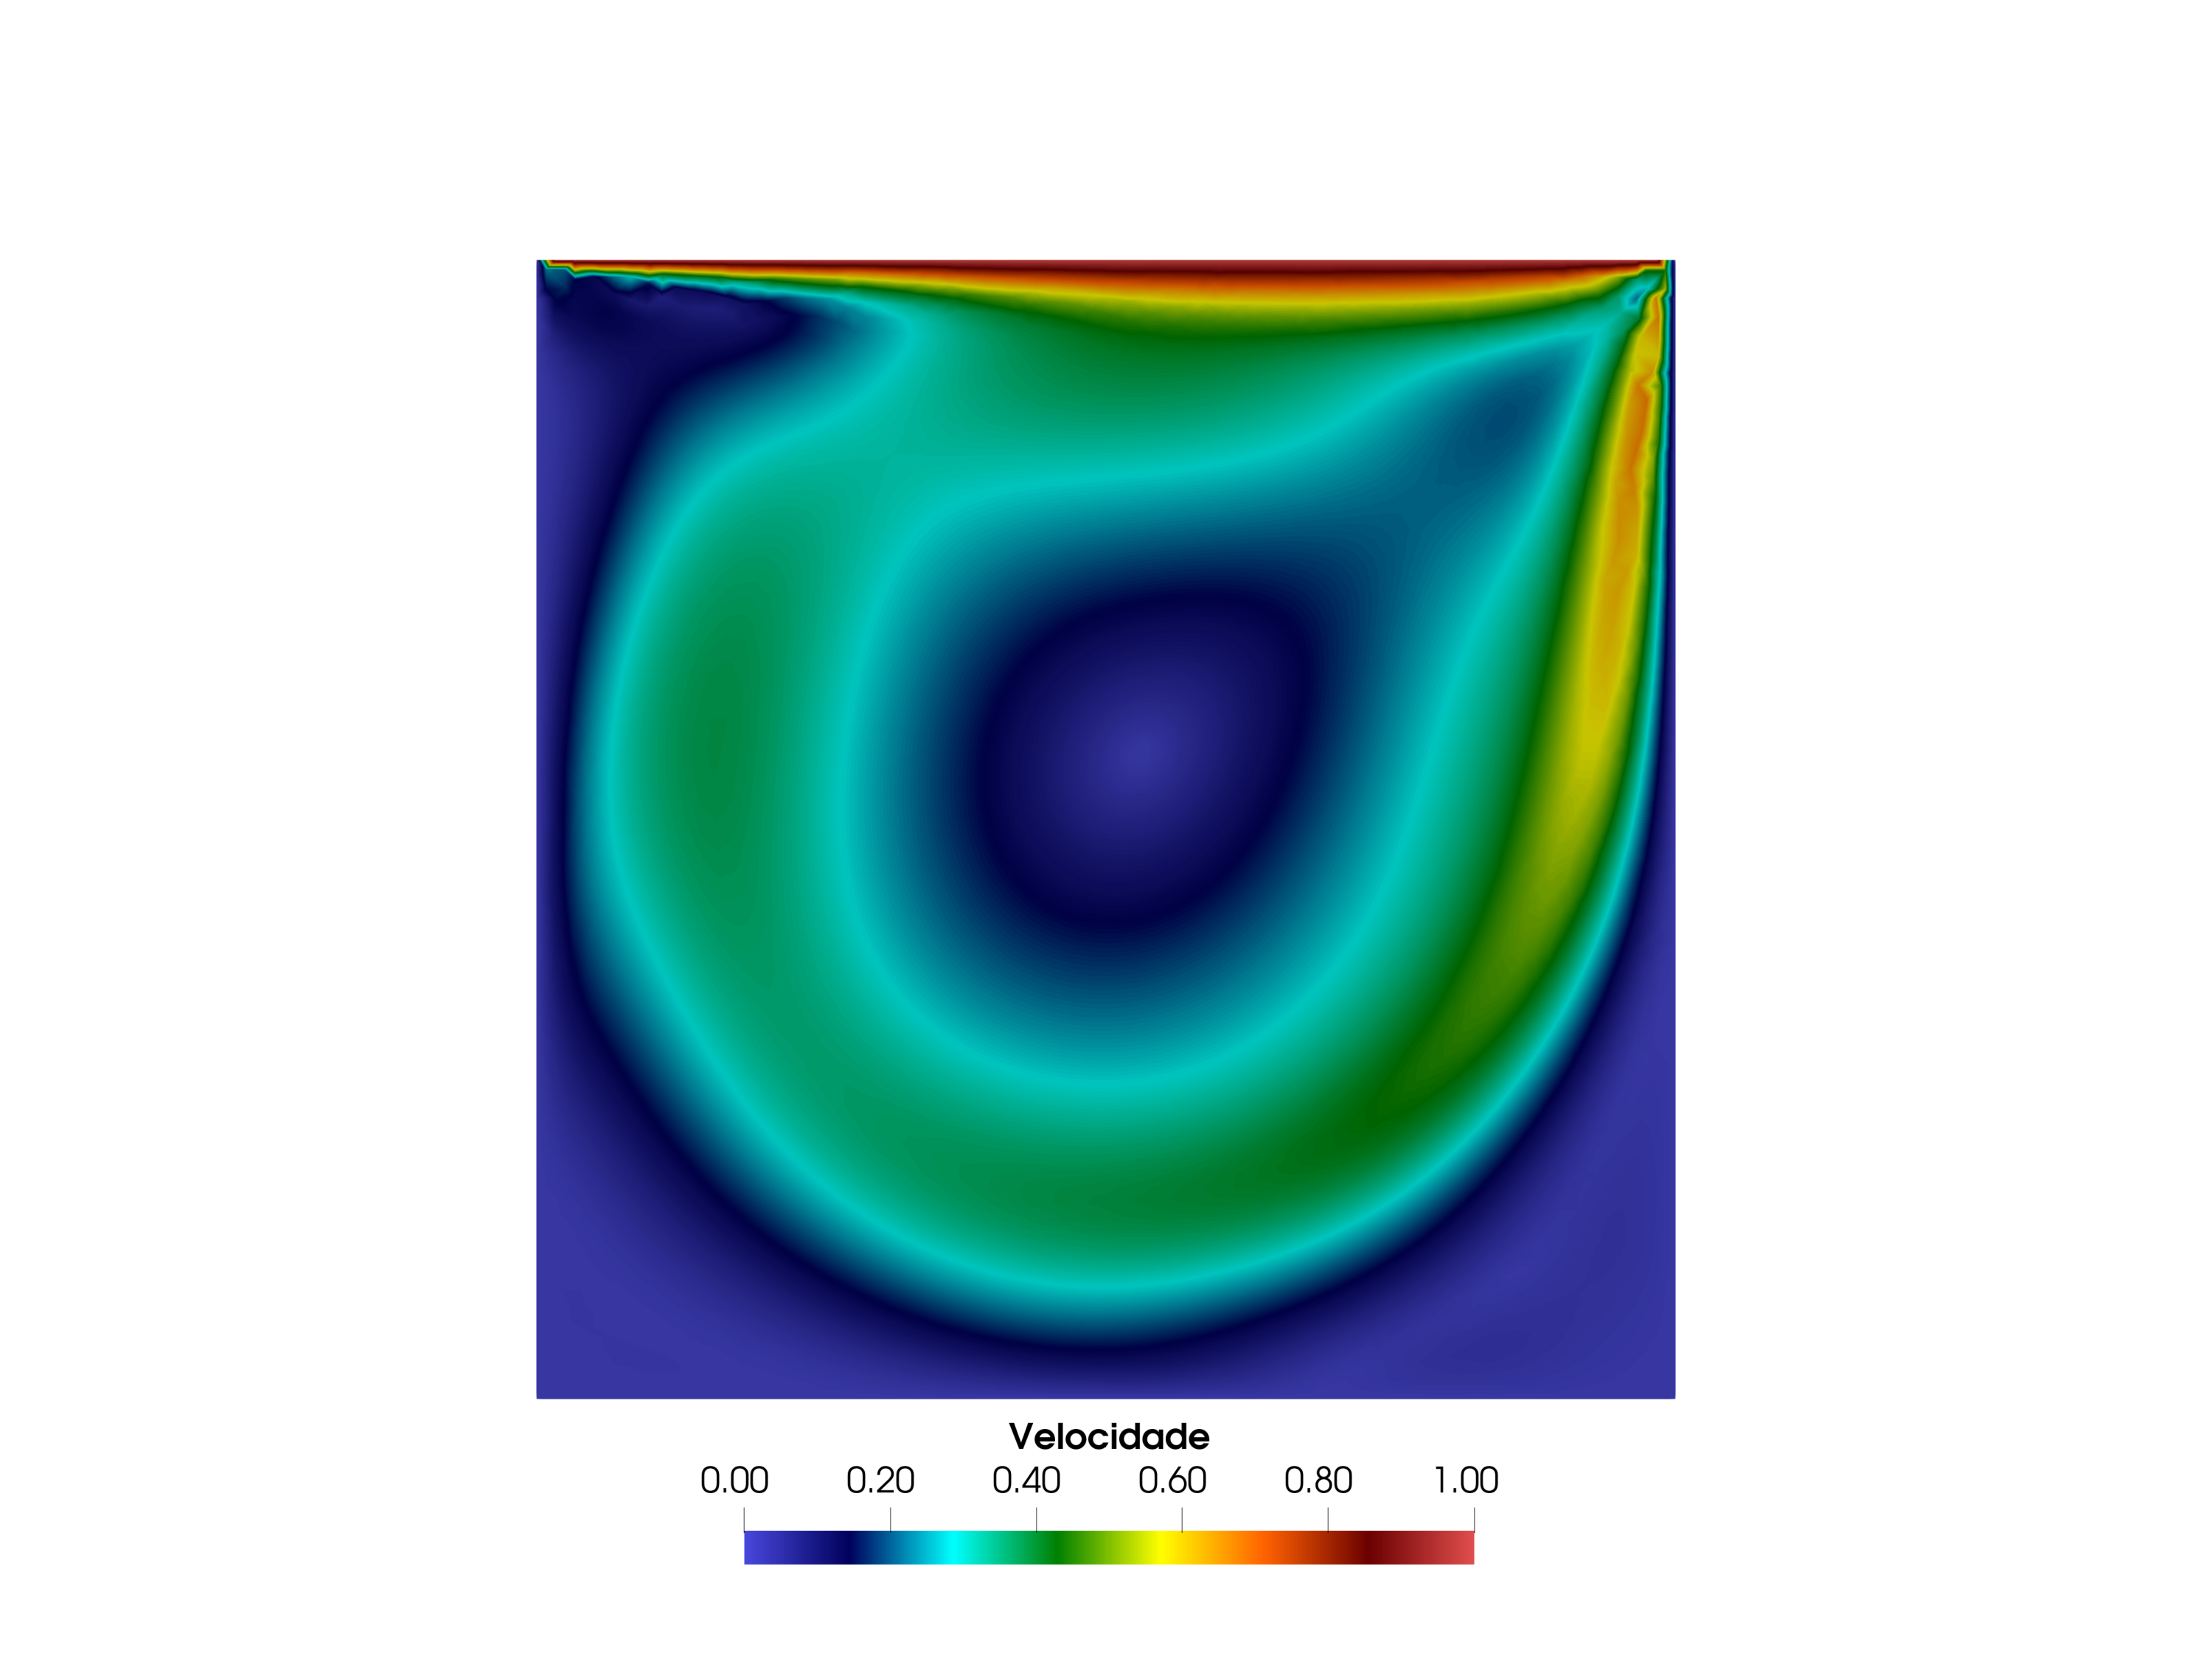
\includegraphics[scale=0.4,trim=12cm 0cm 12cm 32.5cm, clip=true]{Imagens/Cap2/cavidade_velRe1000.pdf}
	\caption{Cavidade quadrada: Campos de velocidade -  plano $y_1$$y_2$}
	\label{fig:cavidade_vel}
\end{figure}

\begin{figure}[!t]
	\centering
	\setlength{\lineskip}{-10pt}
	\subfloat[\label{fig:cavidade_press_Re100}$Re$=100]{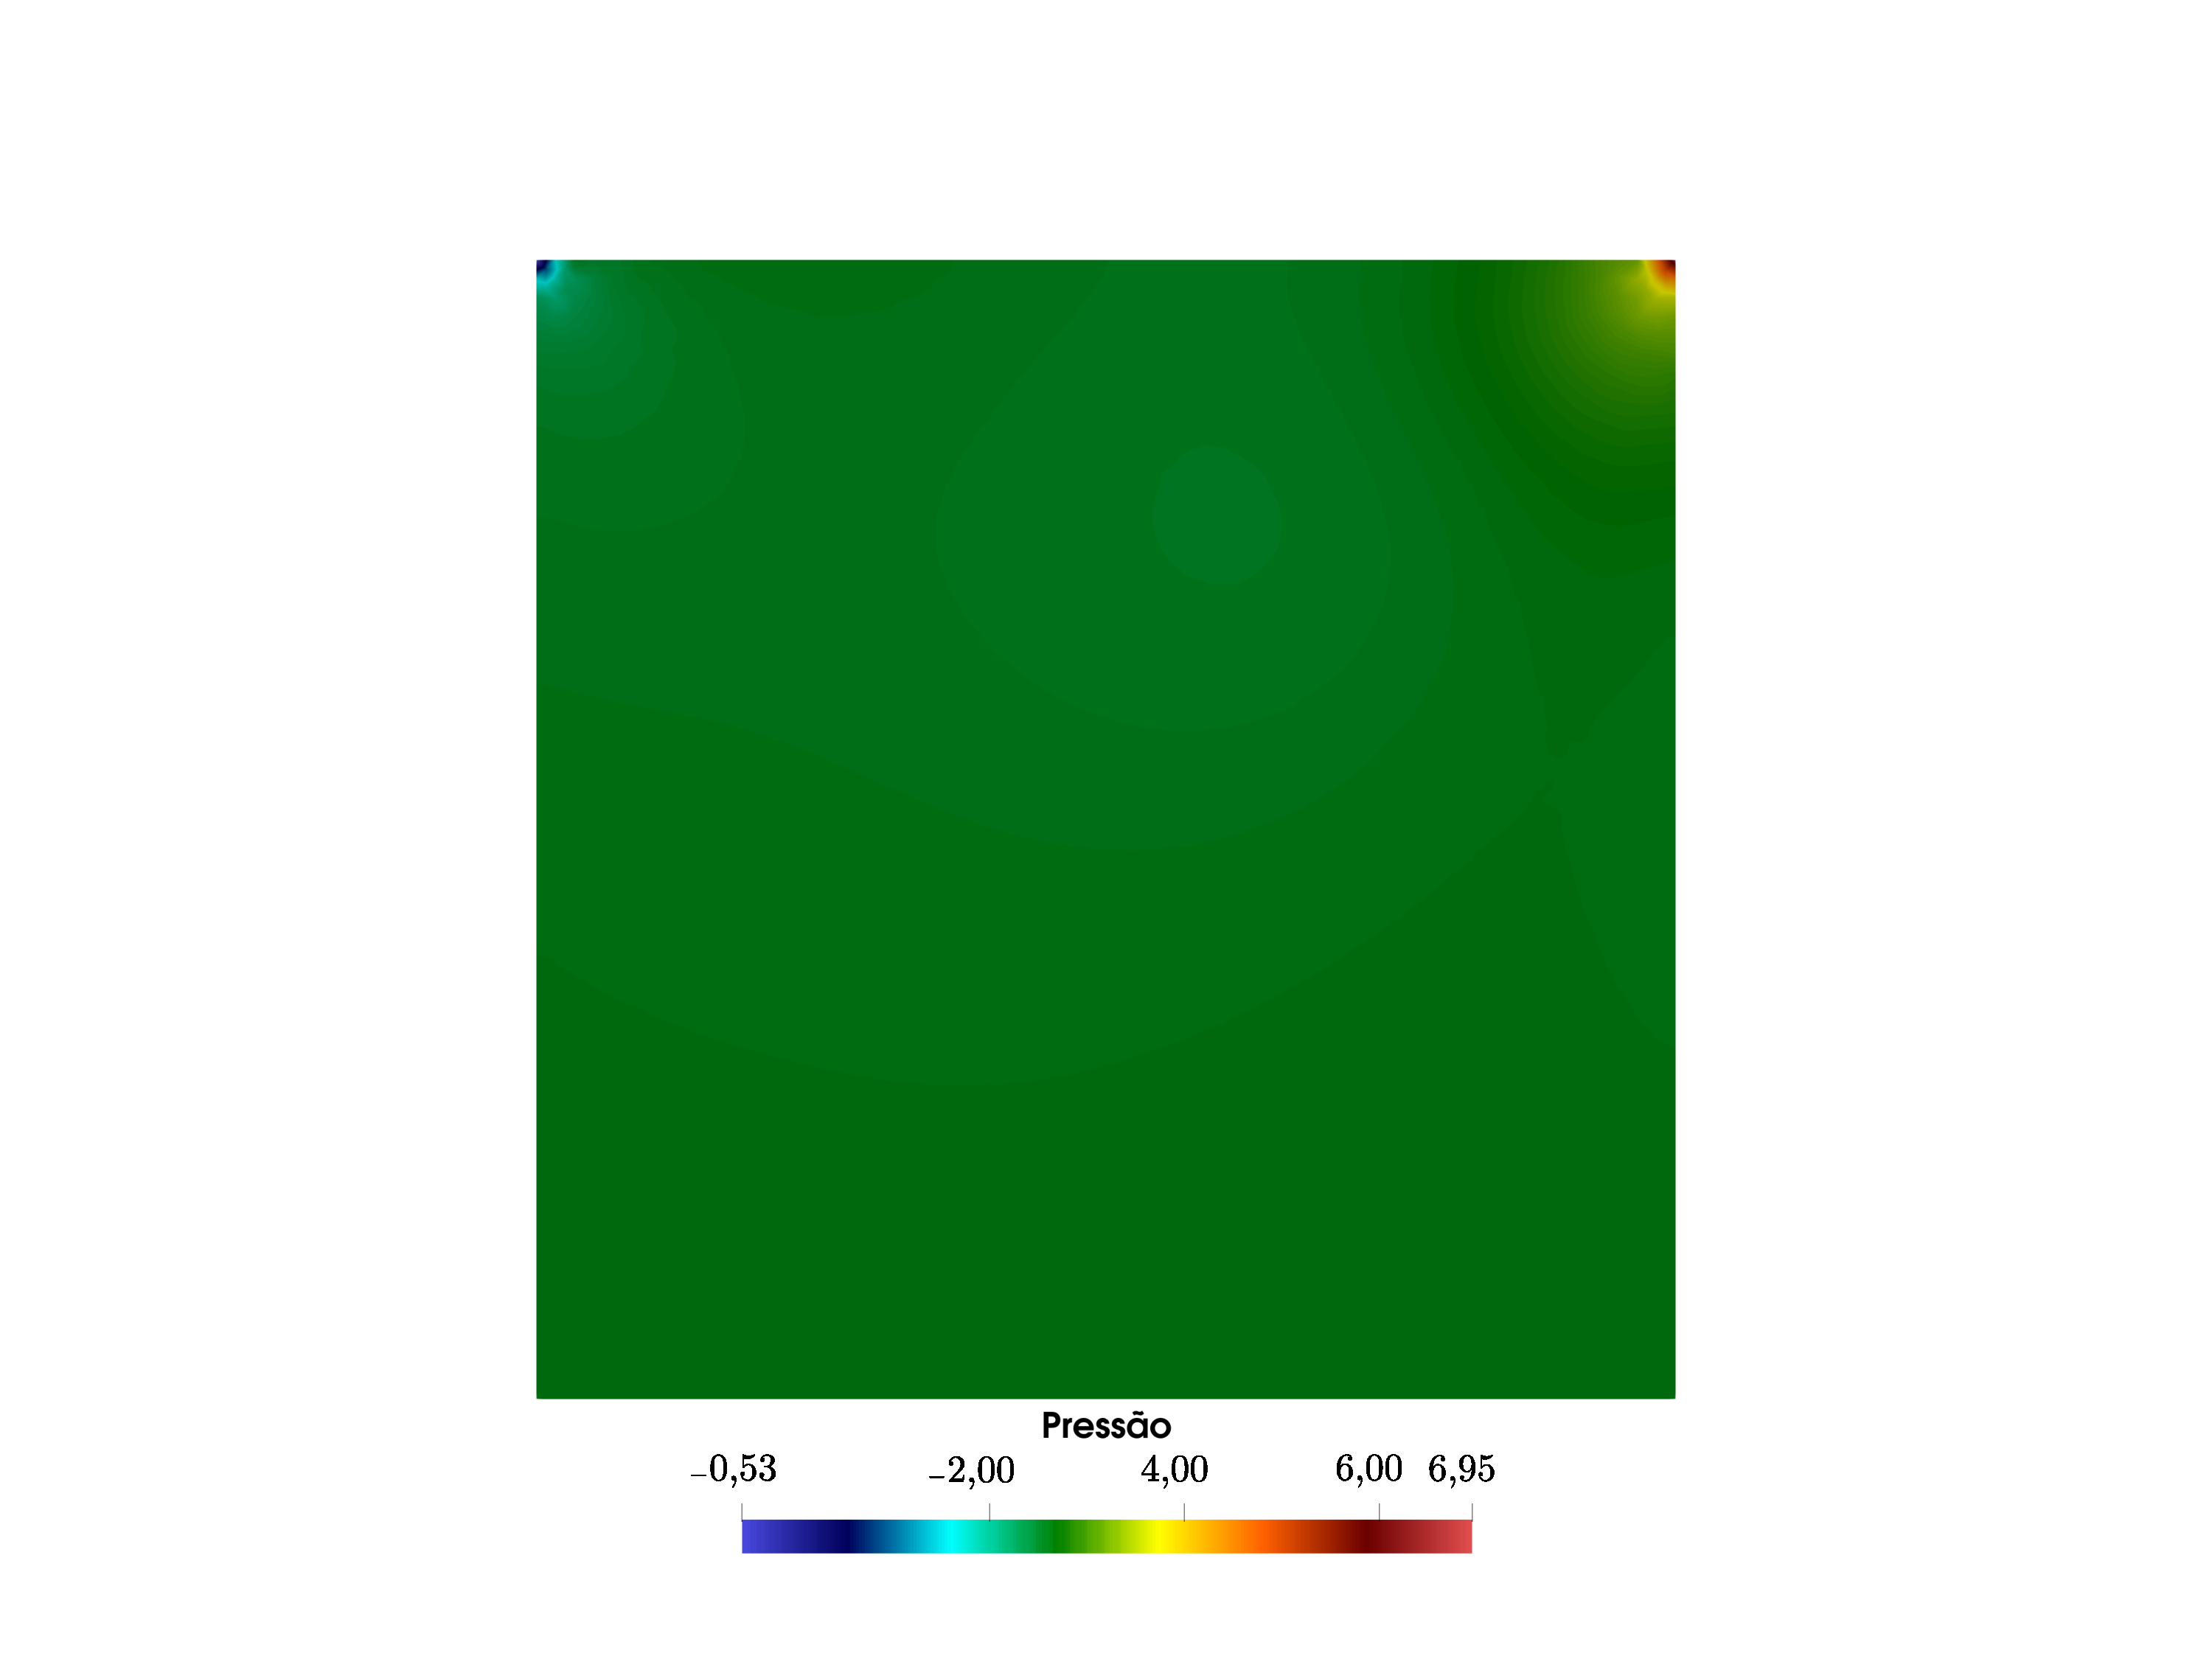
\includegraphics[scale=0.25,trim=12cm 2cm 12cm 5cm, clip=true]{Imagens/Cap2/cavidade_pressRe100.pdf}} 
	\subfloat[\label{fig:cavidade_press_Re400}$Re$=400]{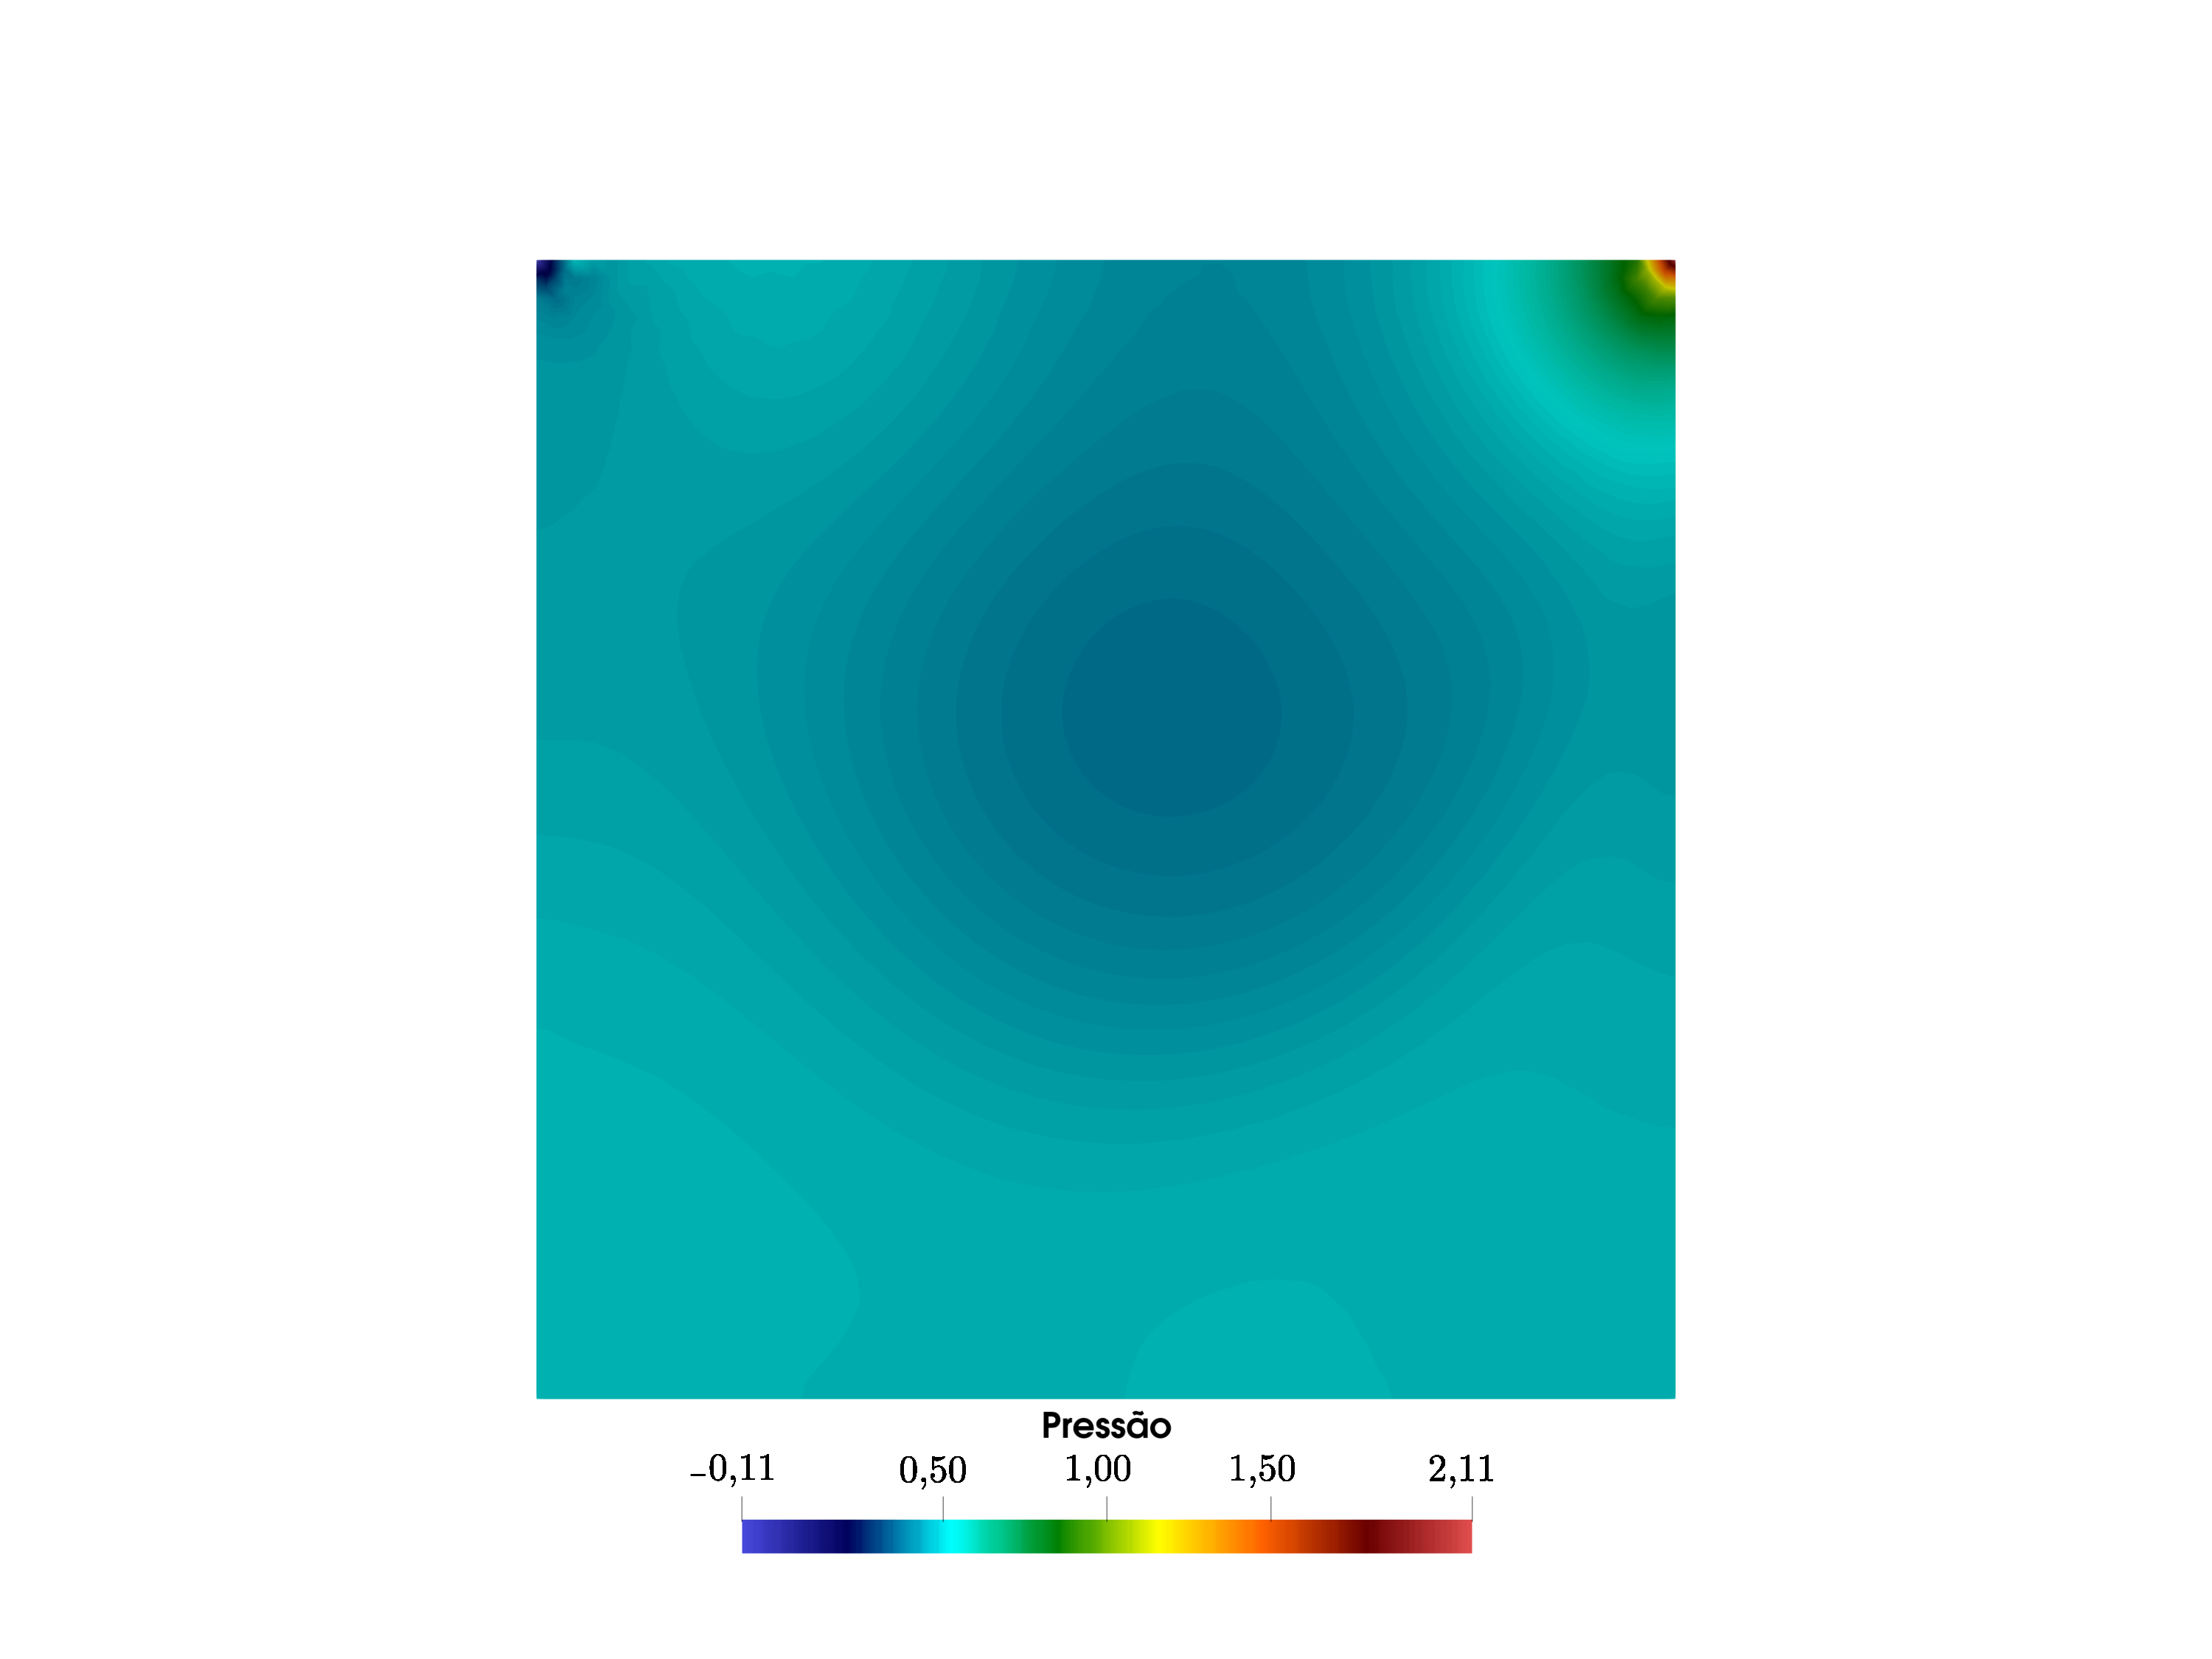
\includegraphics[scale=0.25,trim=12cm 2cm 12cm 5cm, clip=true]{Imagens/Cap2/cavidade_pressRe400.pdf}}\\ 
	\subfloat[\label{fig:cavidade_press_Re1000}$Re$=1000]{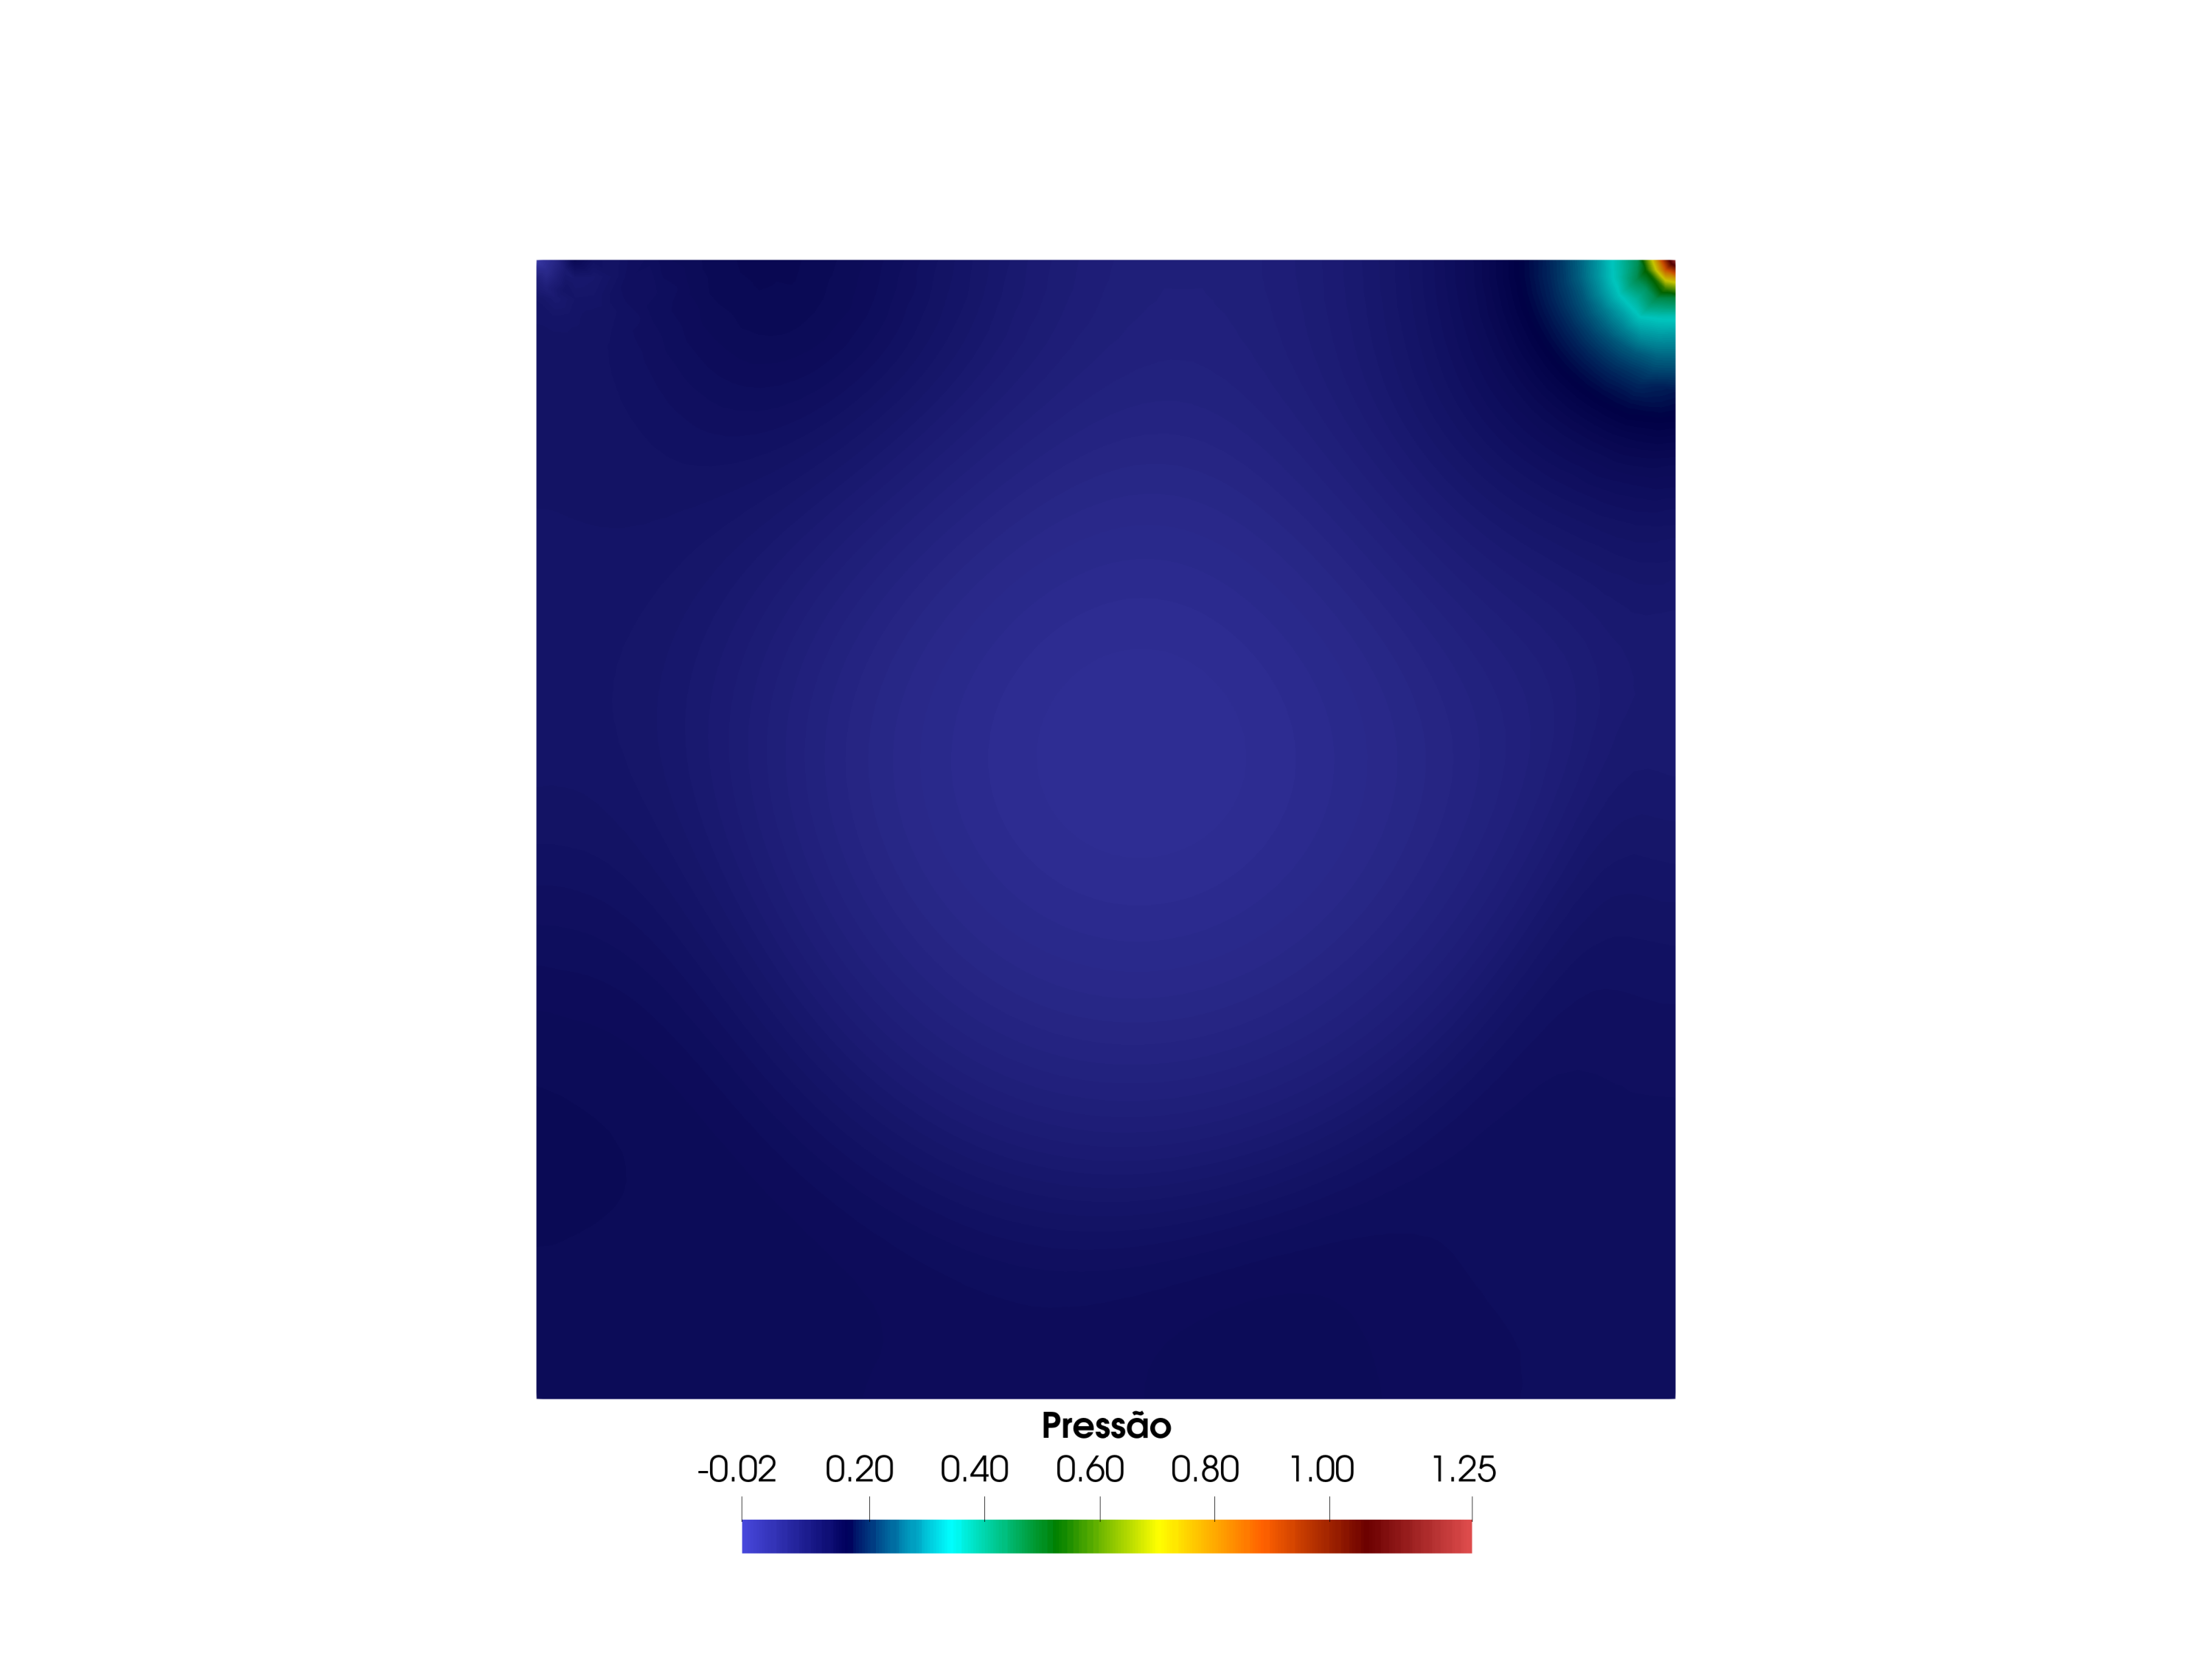
\includegraphics[scale=0.25,trim=12cm 2cm 12cm 5cm, clip=true]{Imagens/Cap2/cavidade_pressRe1000.pdf}}
	\caption{Cavidade quadrada: Campos de pressão - plano $y_1$$y_2$}
	\label{fig:cavidade_press}
\end{figure}



%
%\clearpage[e ]
%
%\textcolor{white}{ }


\end{document}
